%%%%%%%%%%%%%%%%%%%%%%%%%%%%%%%%%%%%%%%%%%%%%%%%%%%%%%%%%%%%%%%%%%%%
% Diskussion und Ausblick
%%%%%%%%%%%%%%%%%%%%%%%%%%%%%%%%%%%%%%%%%%%%%%%%%%%%%%%%%%%%%%%%%%%%

\chapter{Results}
  \label{Results}

\section{WSI networks}

\ref{fig:1FCmodel} shows the results of the ResNet-based model, with only one fully connected layer following the residual blocks. In \ref{fig:1fc_overfit}, the model was run on a small subset ($n=35)$ of the full dataset, to verify the capabilities of the model. \ref{fig:1fc_normal} shows the training results on the full dataset. Both experiments were run for 500 epochs and each took around 15 hours to finish.  
When comparing the loss curves, we notice that the training and validation loss starts to diverge around epoch 75 in figure \ref{fig:1fc_overfit} but not in figure \ref{fig:1fc_normal}. Additionally, we notice that in both cases the validation loss stays above the training loss, with the training loss reaching similar values of 0.14 and 0.13 for full and reduced dataset respectively. Also notable is, that the initial losses are identical when training on the whole dataset but different on the subset intended for overfitting the model.
The achieved concordance indices are indicated in table \ref{tab:c_indices}

\begin{table}[hb!]
    \centering
    \caption{Latest recorded concordance indices for experiments related to unimodal WSI data.}
    \begin{tabular}{l | c c}
       Experiment & Training & Validation  \\ [0.5ex] 
       \hline  
        1 FCL Overfit & 0.93 & 0.78 \\ 
        1 FCL Normal & 0.86 & 0.89 \\
        2 FCL lr 0.01 & 0.86 & 0.89 \\
        2 FCL lr 0.001 & 0.84 & 0.78 \\
        EfficientNet & 0.82 & 0.93 \\
        \hline
    \end{tabular}
    \label{tab:c_indices}
\end{table}


\begin{figure}[h!t]
    \centering
     \begin{subfigure}[b]{0.495\textwidth}
         \centering
         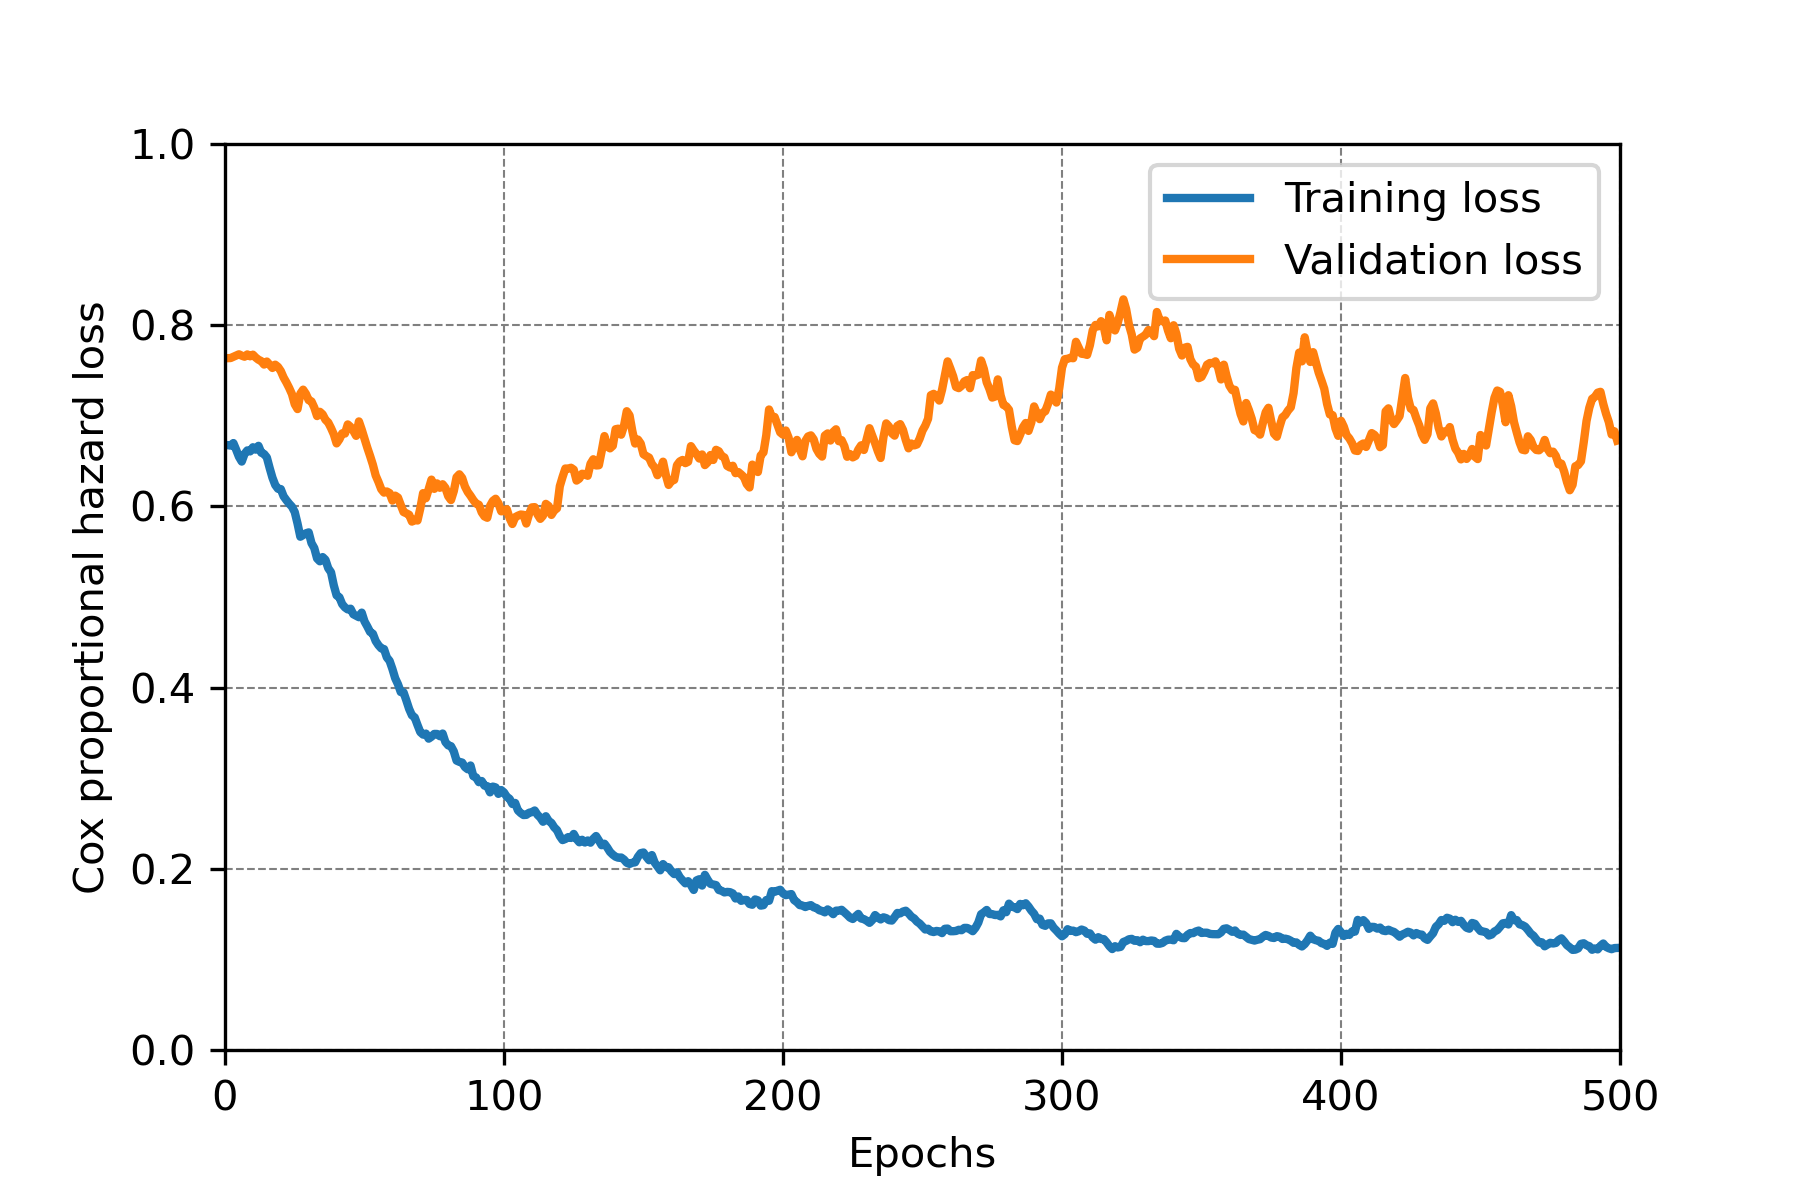
\includegraphics[width=\textwidth]{latex/loss_plots/!!!_overfit0.05.png}
         \caption{Overfitting on subset of data}
         \label{fig:1fc_overfit}
     \end{subfigure}
    \hfill
     \begin{subfigure}[b]{0.495\textwidth}
         \centering
         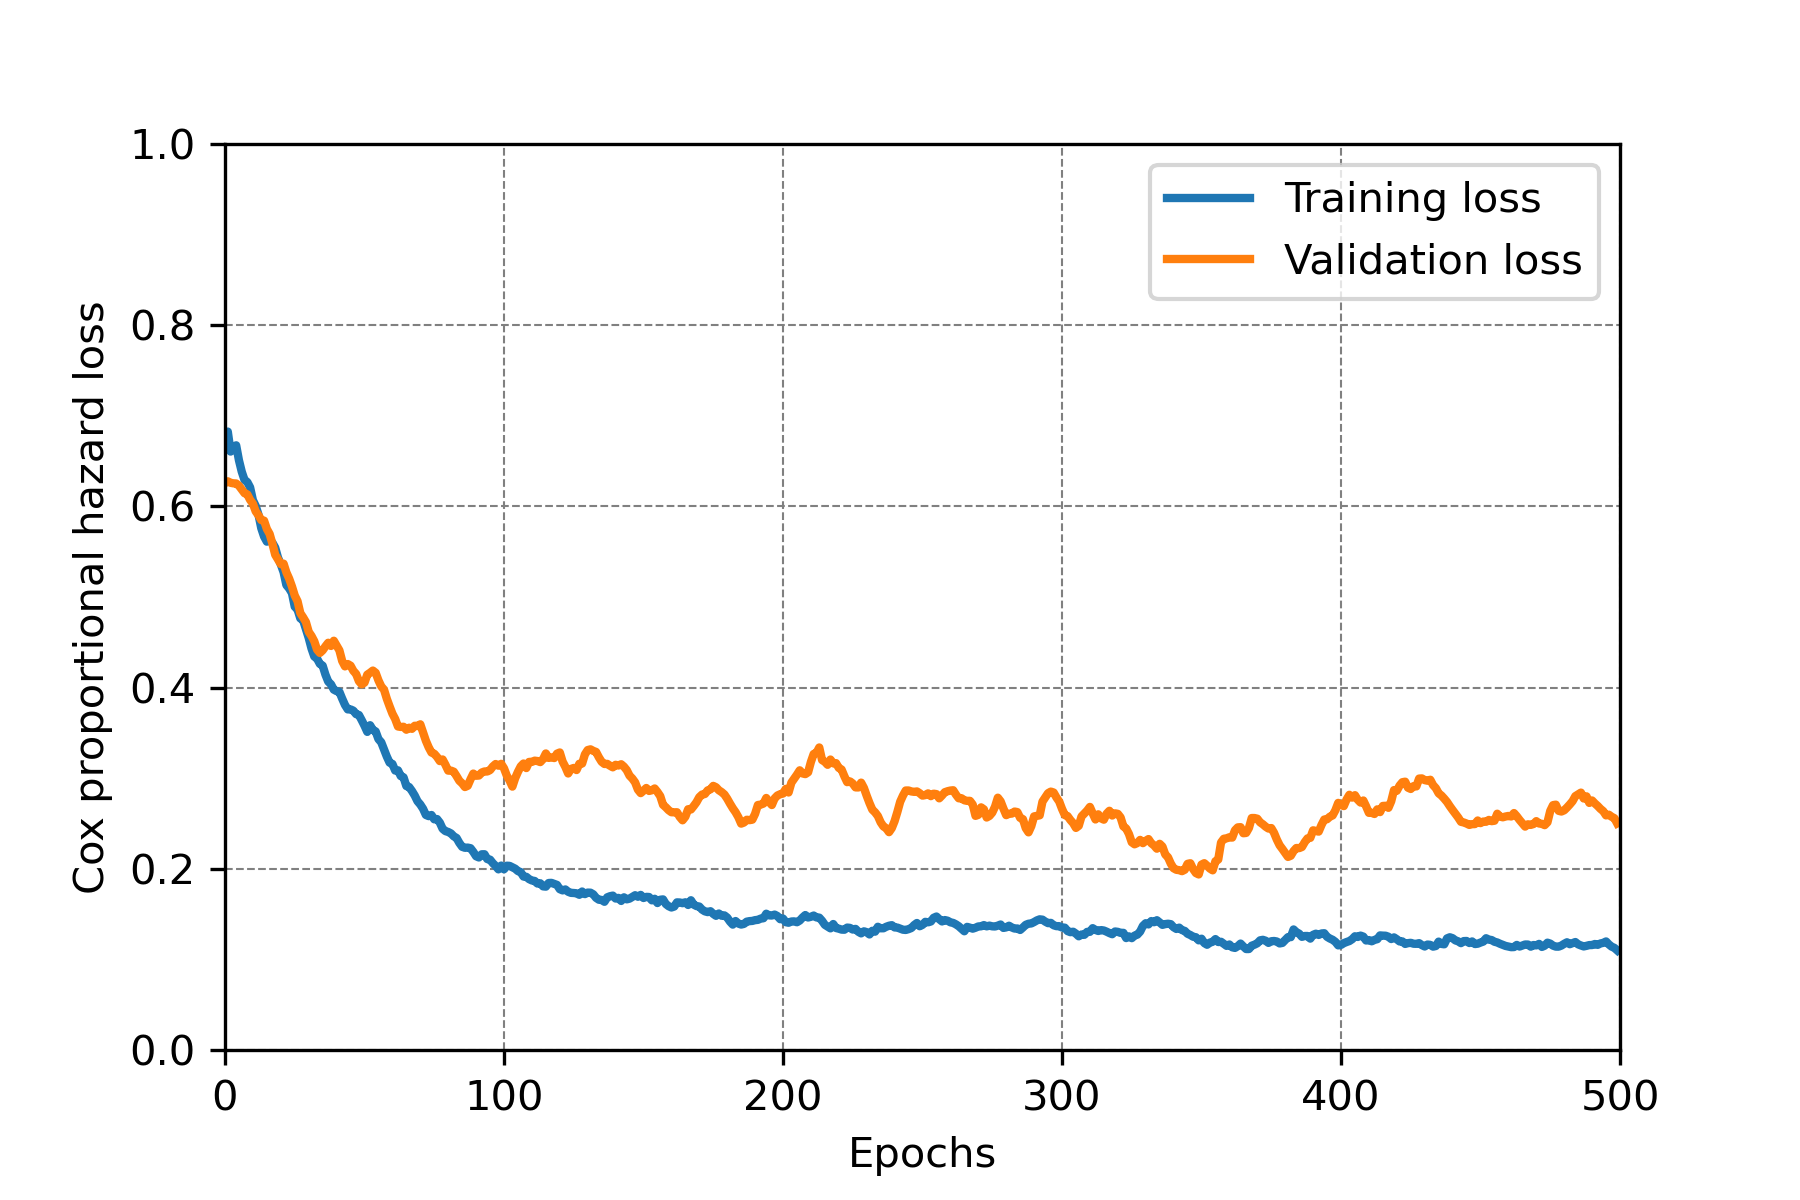
\includegraphics[width=\textwidth]{latex/loss_plots/!!!_2023-04-03.png}
         \caption{Training on whole dataset}
         \label{fig:1fc_normal}
     \end{subfigure}
    \hfill
    \caption[CNN with Single-Layer Prediction]{Results of ResNet based CNN using a single fully connected output layer. Figure \ref{fig:1fc_overfit} shows the results of overfitting the network on 5\% of data (n=35). Figure \ref{fig:1fc_normal} shows the results for training on the full dataset.}
    \label{fig:1FCmodel}
\end{figure}

The experiment was repeated with the ResNet architecture replaced with a model that was based on EfficientNetV2 \cite{Tan2021EfficientNetV2}. Figure \ref{fig:Effnet} contains the corresponding results. We notice that the concordance index for the validation set overtakes the one for the training set at around 100 epochs, due to a steeper ascend until that point. 

\begin{figure}[h!t]
    \centering
     \begin{subfigure}[b]{0.495\textwidth}
         \centering
         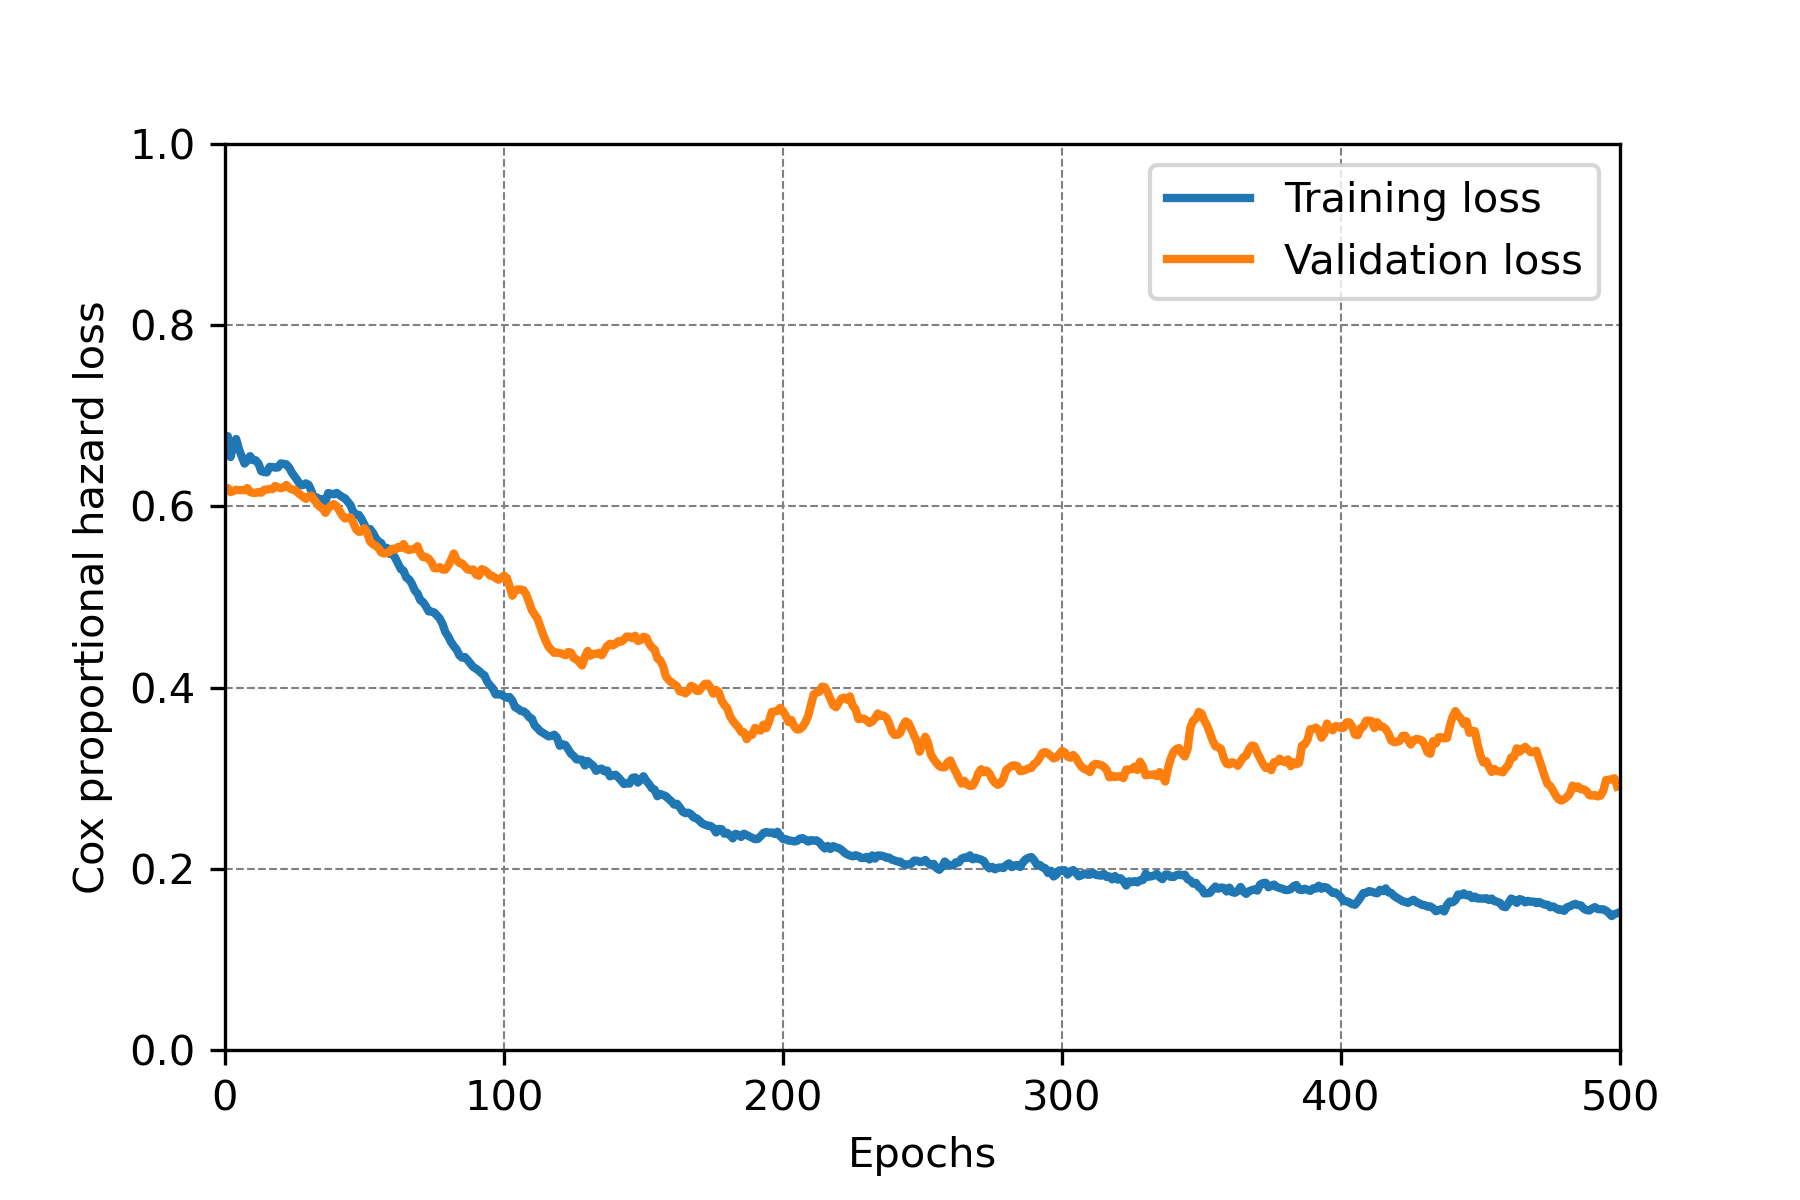
\includegraphics[width=\textwidth]{latex/loss_plots/acc12_lr0.01_effnets.png}
         \caption{Training and validation loss}
         \label{fig:effnetloss}
     \end{subfigure}
    \hfill
     \begin{subfigure}[b]{0.495\textwidth}
         \centering
         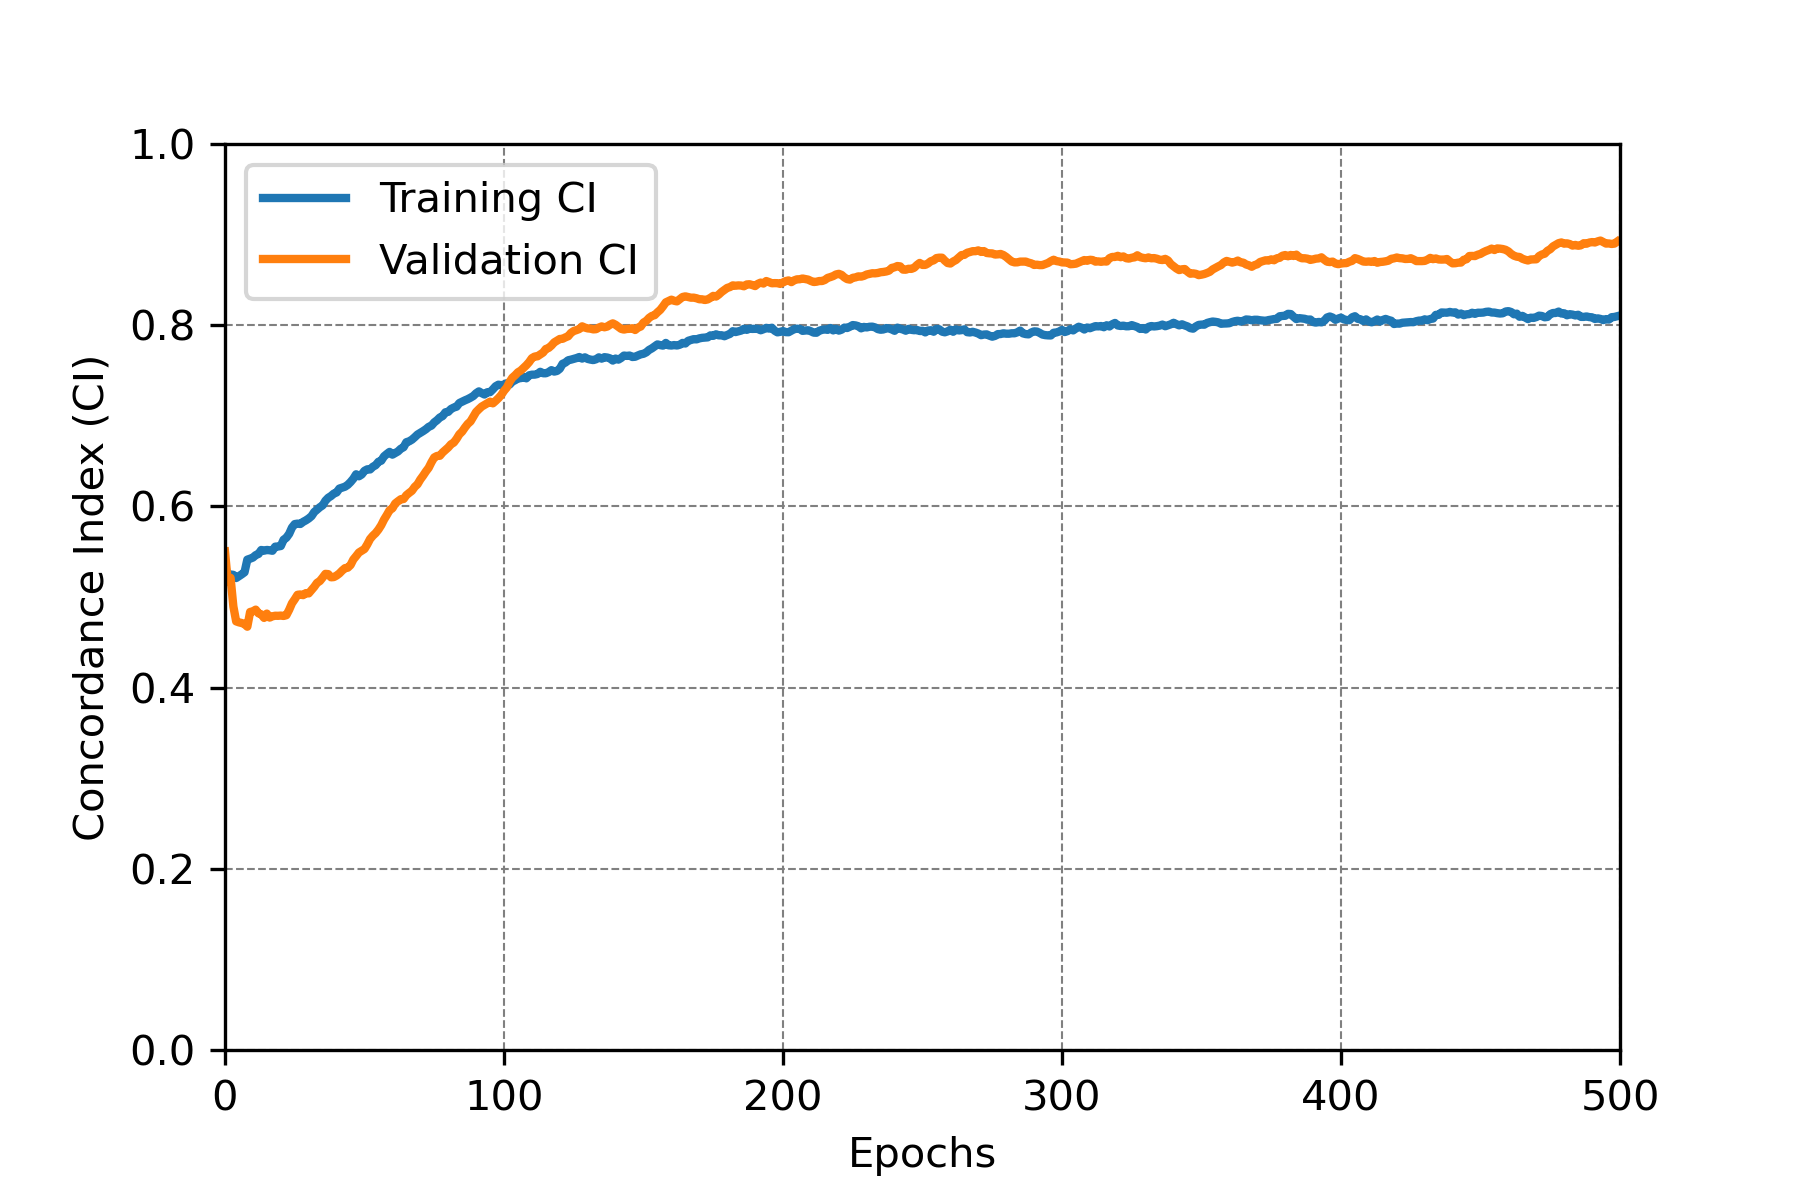
\includegraphics[width=\textwidth]{latex/ci_plots/acc12_lr0.01_effnets.png}
         \caption{Concordance indices}
         \label{fig:effnetci}
     \end{subfigure}
    \hfill
    \caption[EfficientNet with Single-Layer Prediction]{EfficientNet implementation trained on WSI data.}
    \label{fig:Effnet}
\end{figure}


Figure \ref{fig:resnet_lr} shows the second version of our ResNet model, which was later used for the fusion approaches. We tested the model with two different learning rates. When using a learning rate of 0.001, we again notice a divergence of losses after some time. Also, in both settings, the validation loss tracks the training loss very close for a few epochs, after which it diverges. Most notable is the difference in concordance indices, where the learning rate of 0.01 leads to higher values consistently. 
As we considered gradient accumulations necessary to be able to retrieve reliable results despite low batch sizes per iteration, we also experimented with different numbers of accumulation steps. This experiment was conducted at a learning rate of 0.01 and hence is best compared to the previous experiment at the same learning rate since only the number of accumulations differ. We see almost identical results, only the concordance index of the validation data seems to converge faster with less accumulation steps.

\begin{figure}[h!t]
    \centering
 \begin{subfigure}[b]{0.49\textwidth}
     \centering
     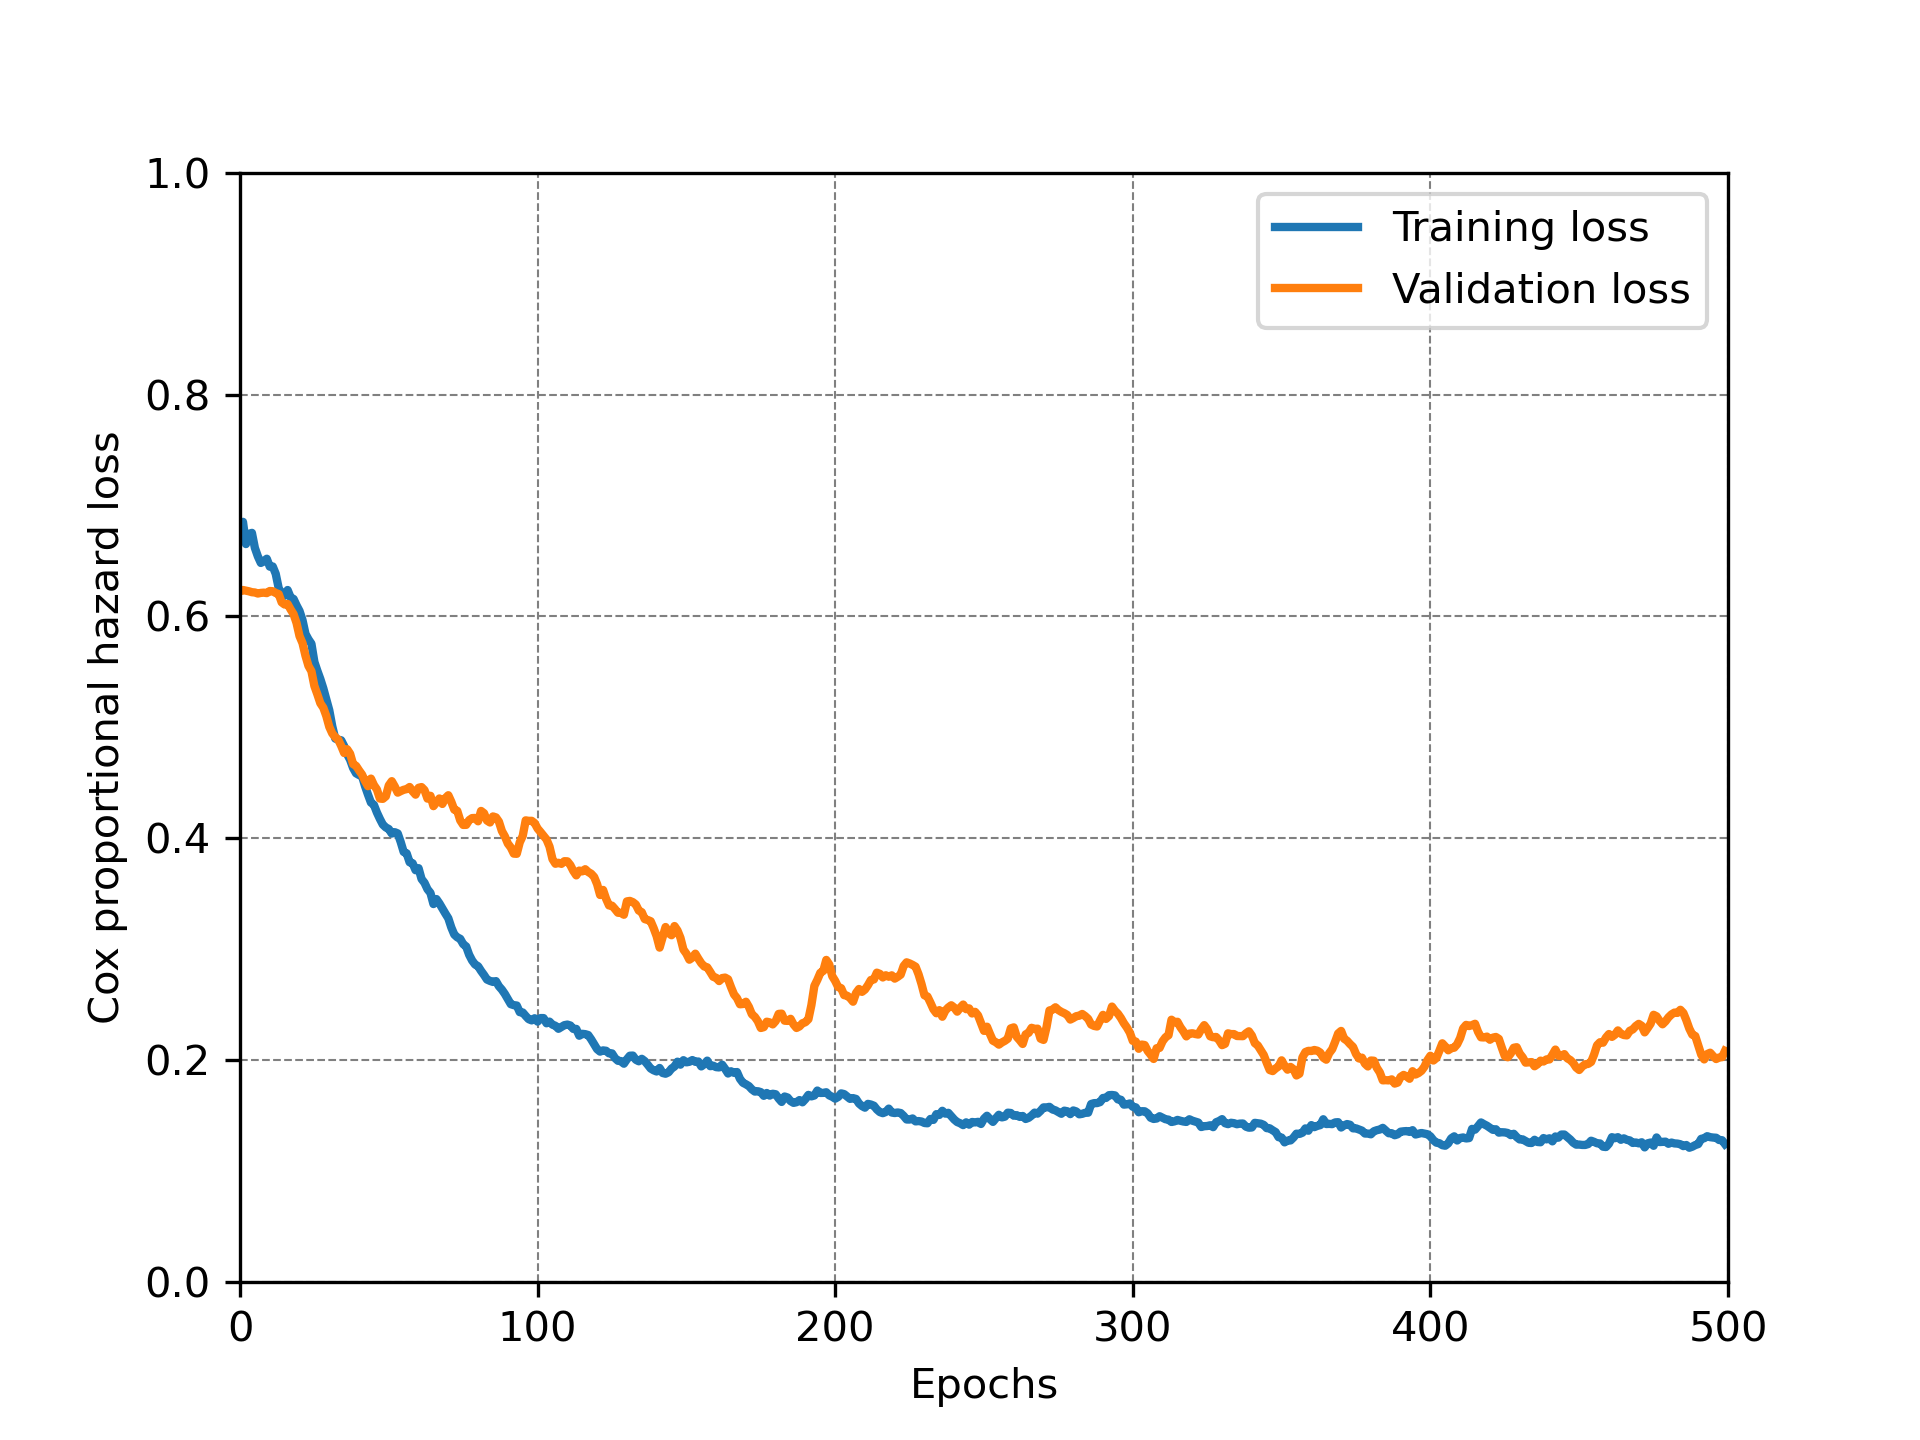
\includegraphics[width=\textwidth]{latex/loss_plots/2FC_lr_0.01.png}
     \caption{Losses at lr 1e-2 and 12 gradient accumulations}
 \end{subfigure}
    \hfill
     \begin{subfigure}[b]{0.49\textwidth}
         \centering
         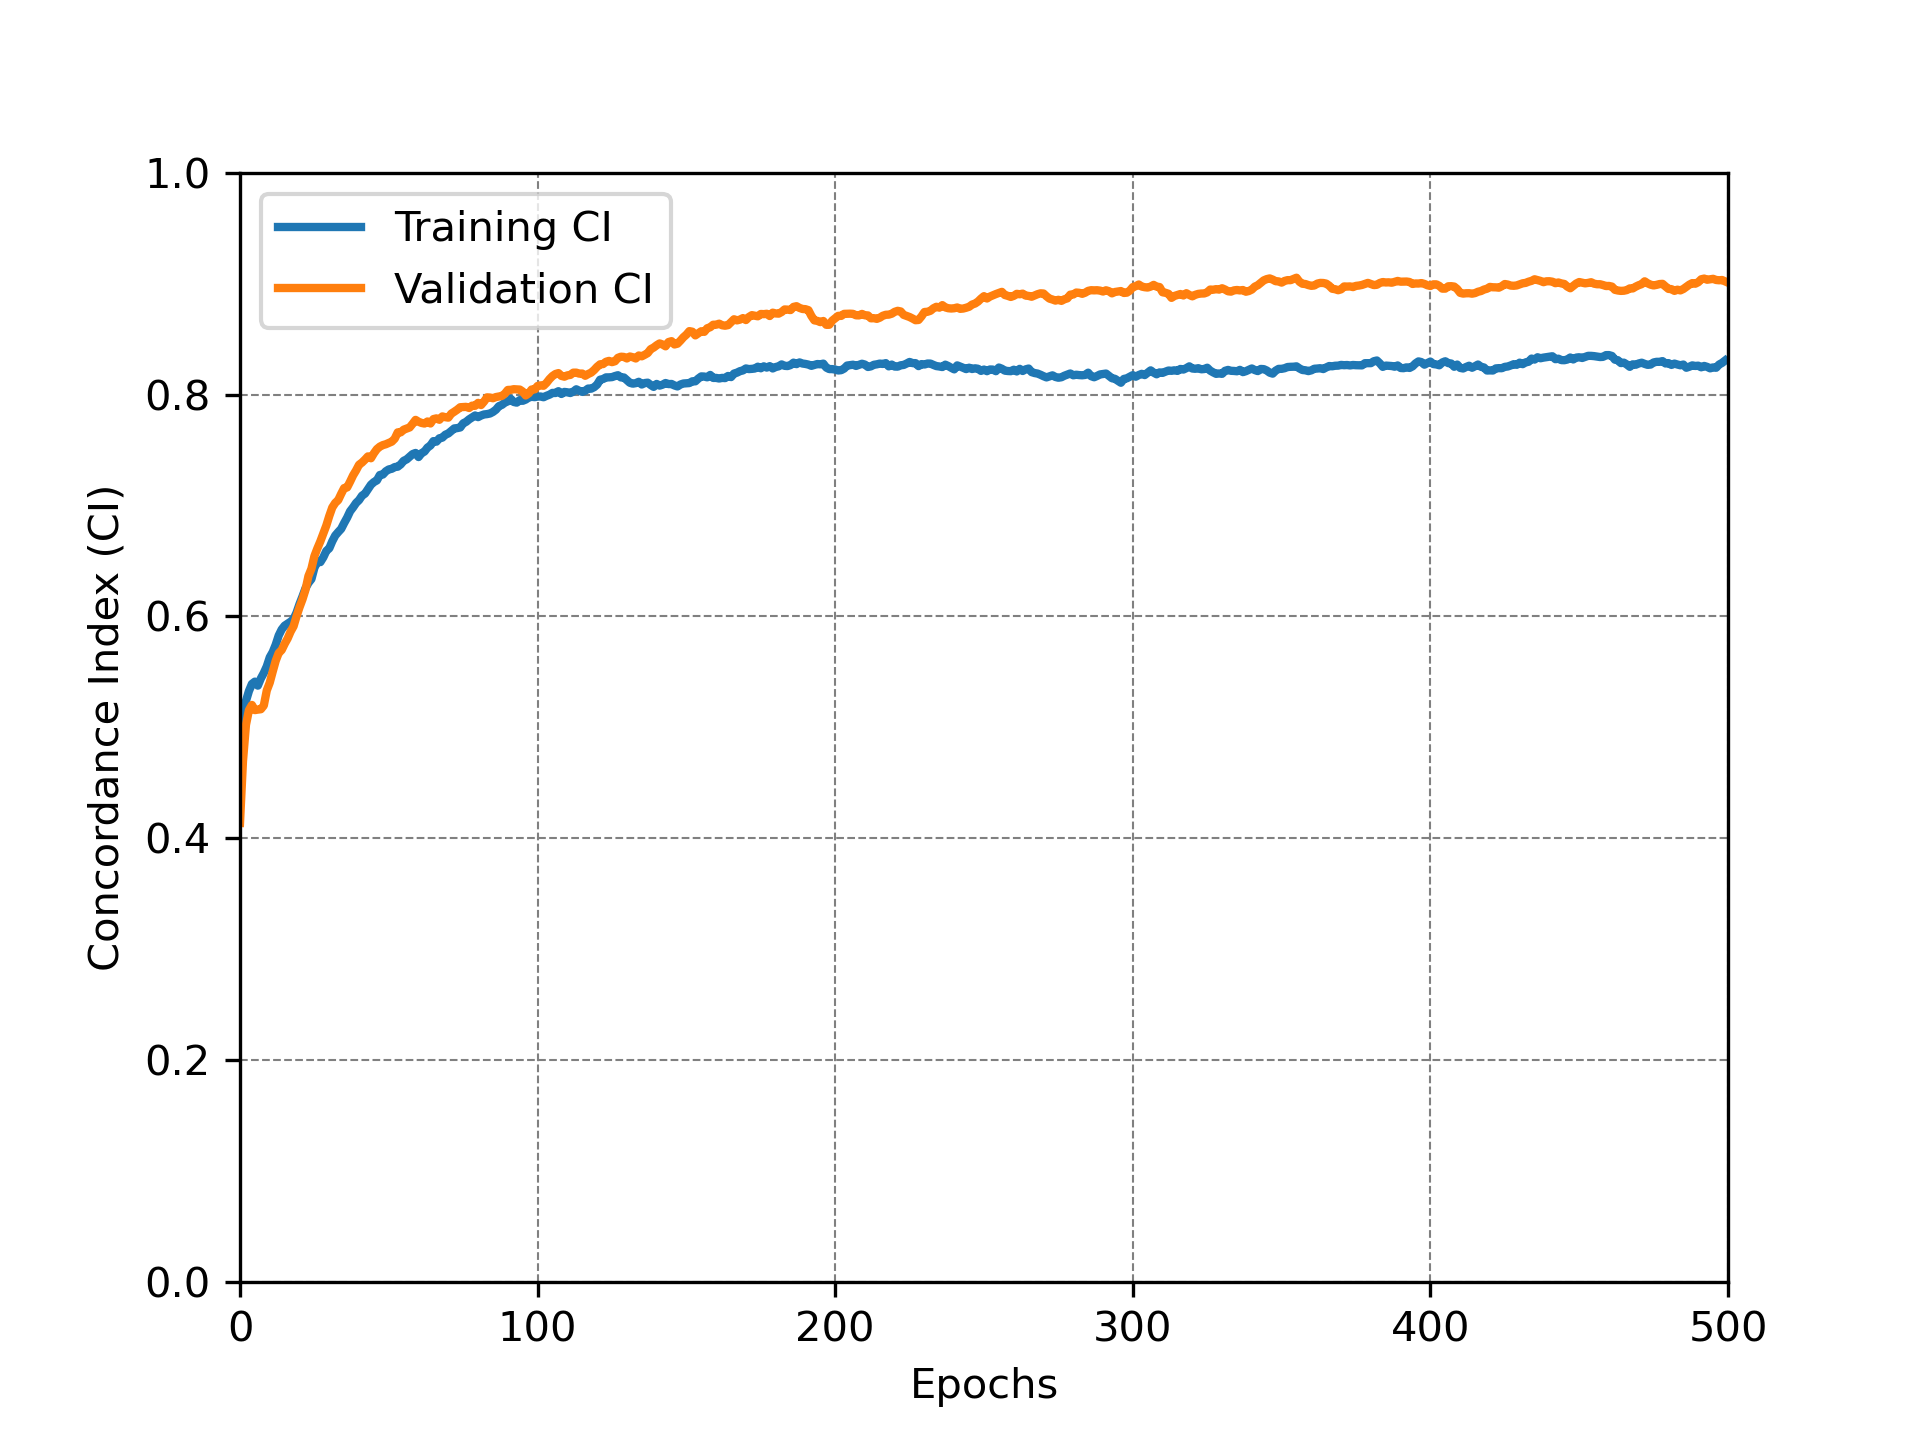
\includegraphics[width=\textwidth]{latex/ci_plots/2FC_lr_0.01.png}
         \caption{Concordance indices at lr 1e-2 and 12 gradient accumulations}
     \end{subfigure}
\vskip\baselineskip
     \begin{subfigure}[b]{0.49\textwidth}
         \centering
         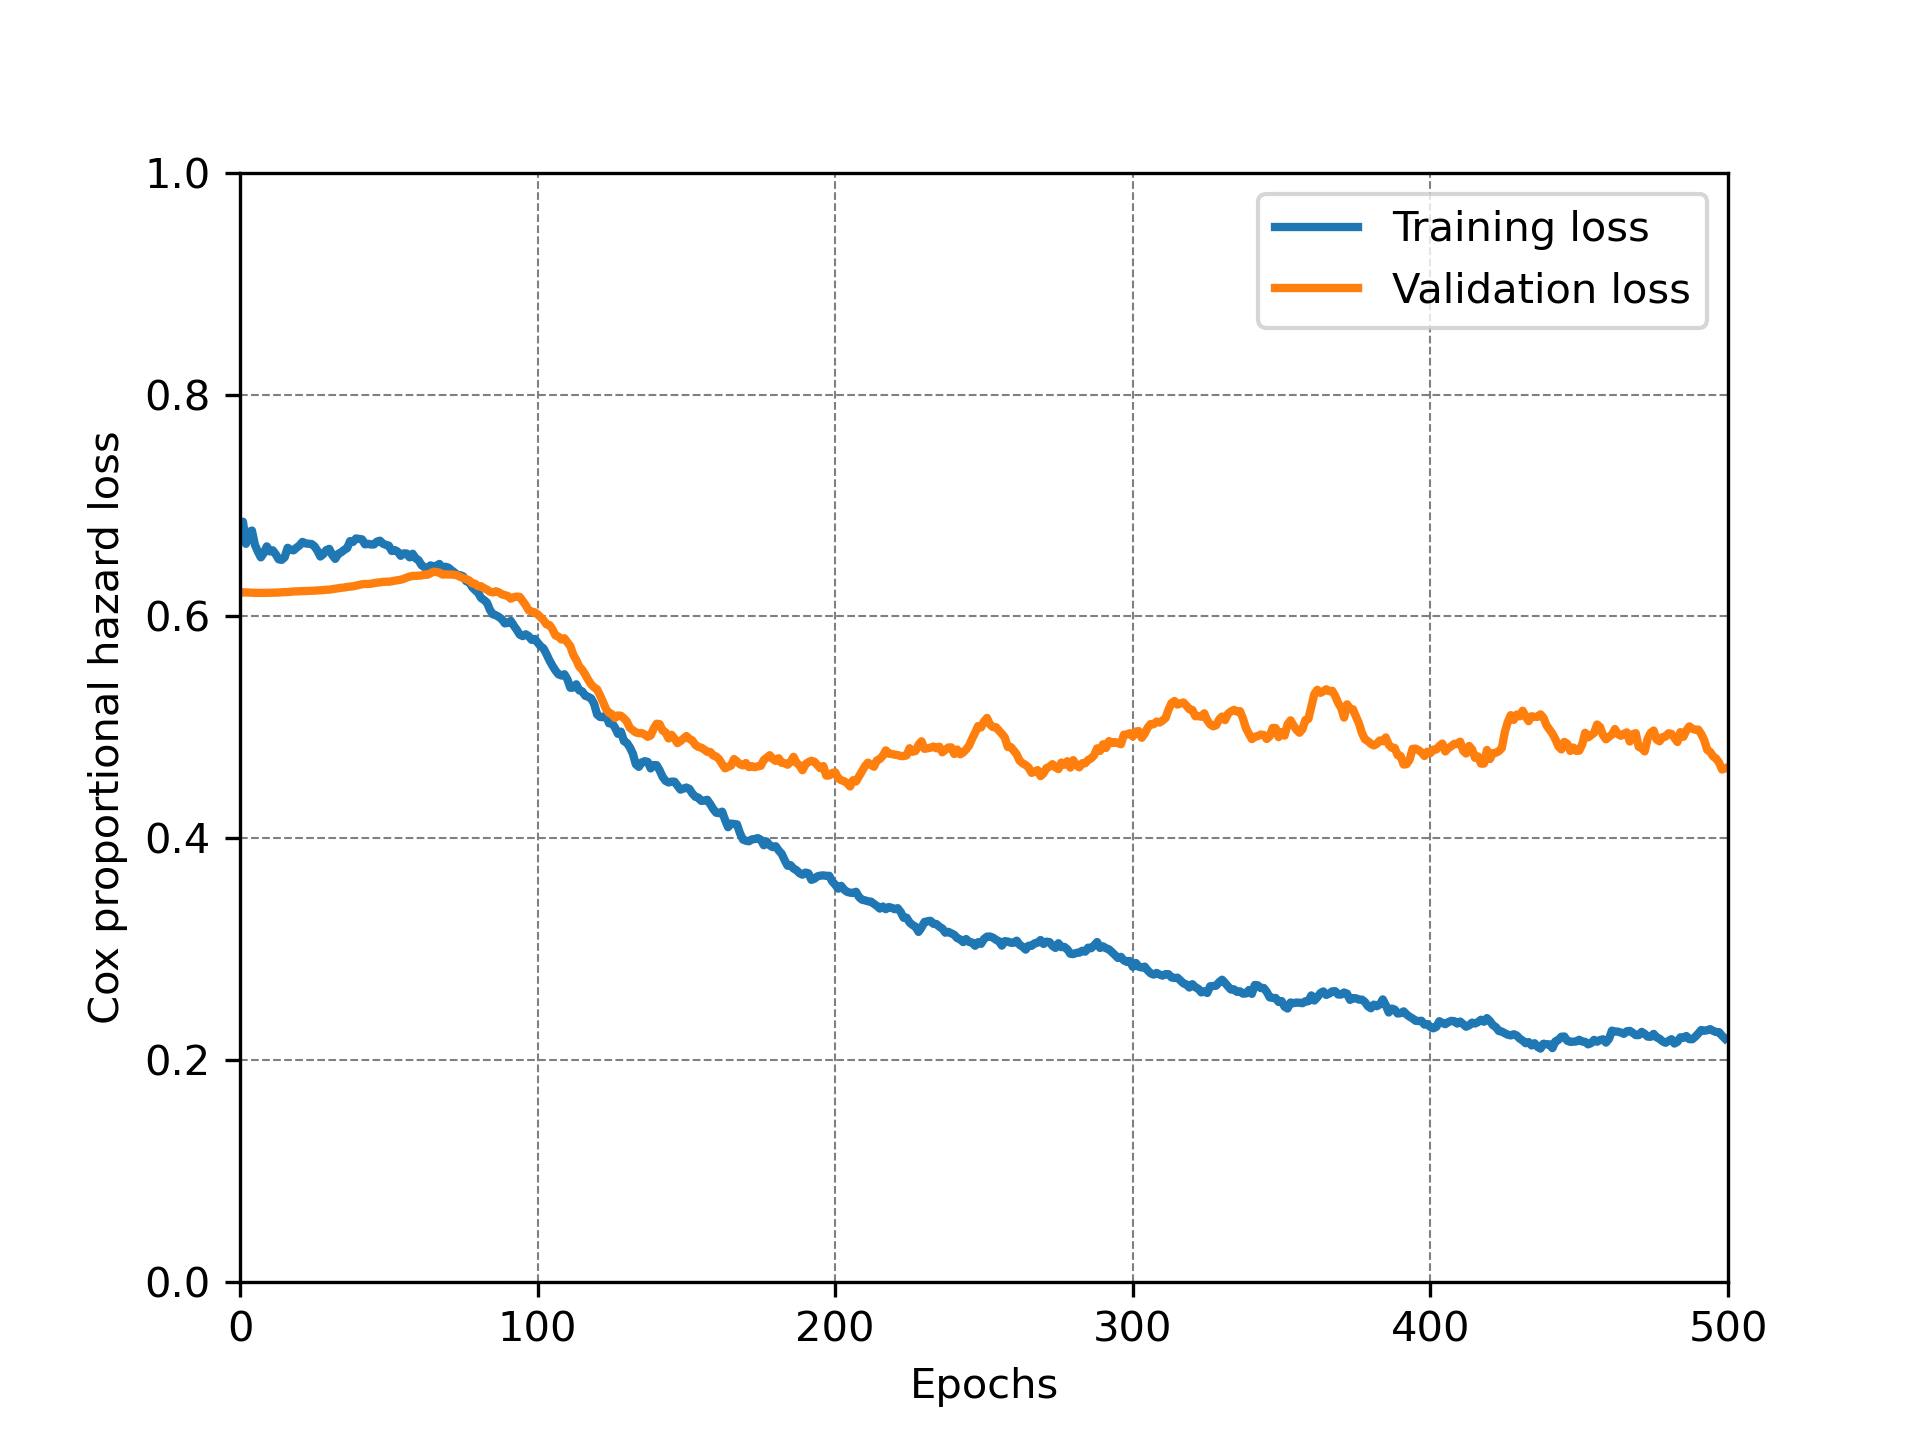
\includegraphics[width=\textwidth]{latex/loss_plots/2FC_lr_0.001.png}
         \caption{Losses at lr 1e-3}
     \end{subfigure}
    \hfill
     \begin{subfigure}[b]{0.49\textwidth}
         \centering
         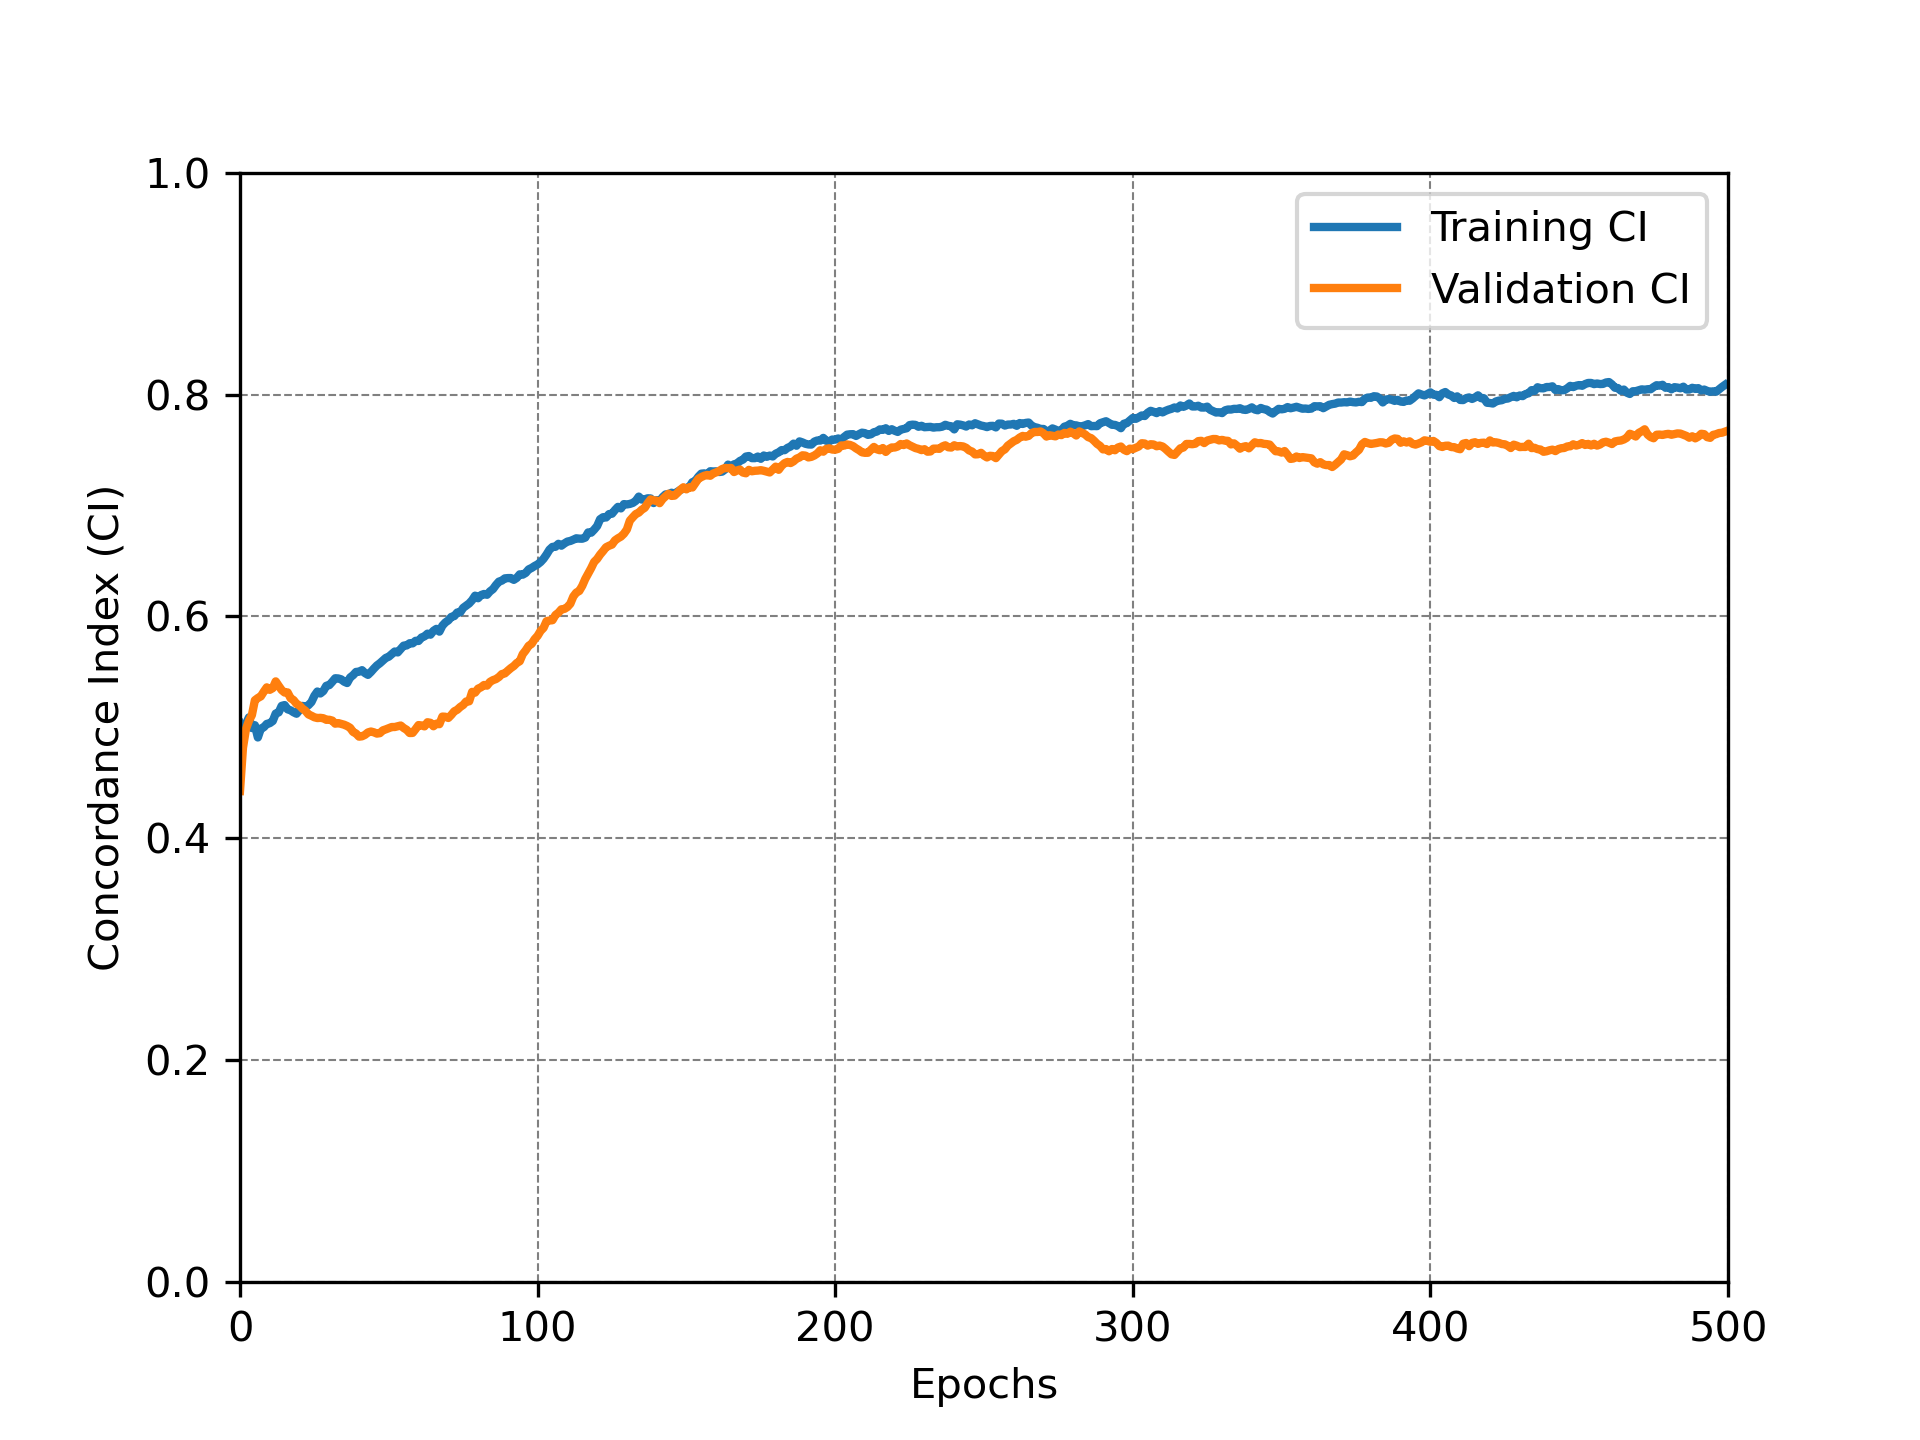
\includegraphics[width=\textwidth]{latex/ci_plots/2FC_lr_0.001.png}
         \caption{Concordance indices at lr 1e-3}
     \end{subfigure}
    \hfill
     \begin{subfigure}[b]{0.49\textwidth}
     \centering
     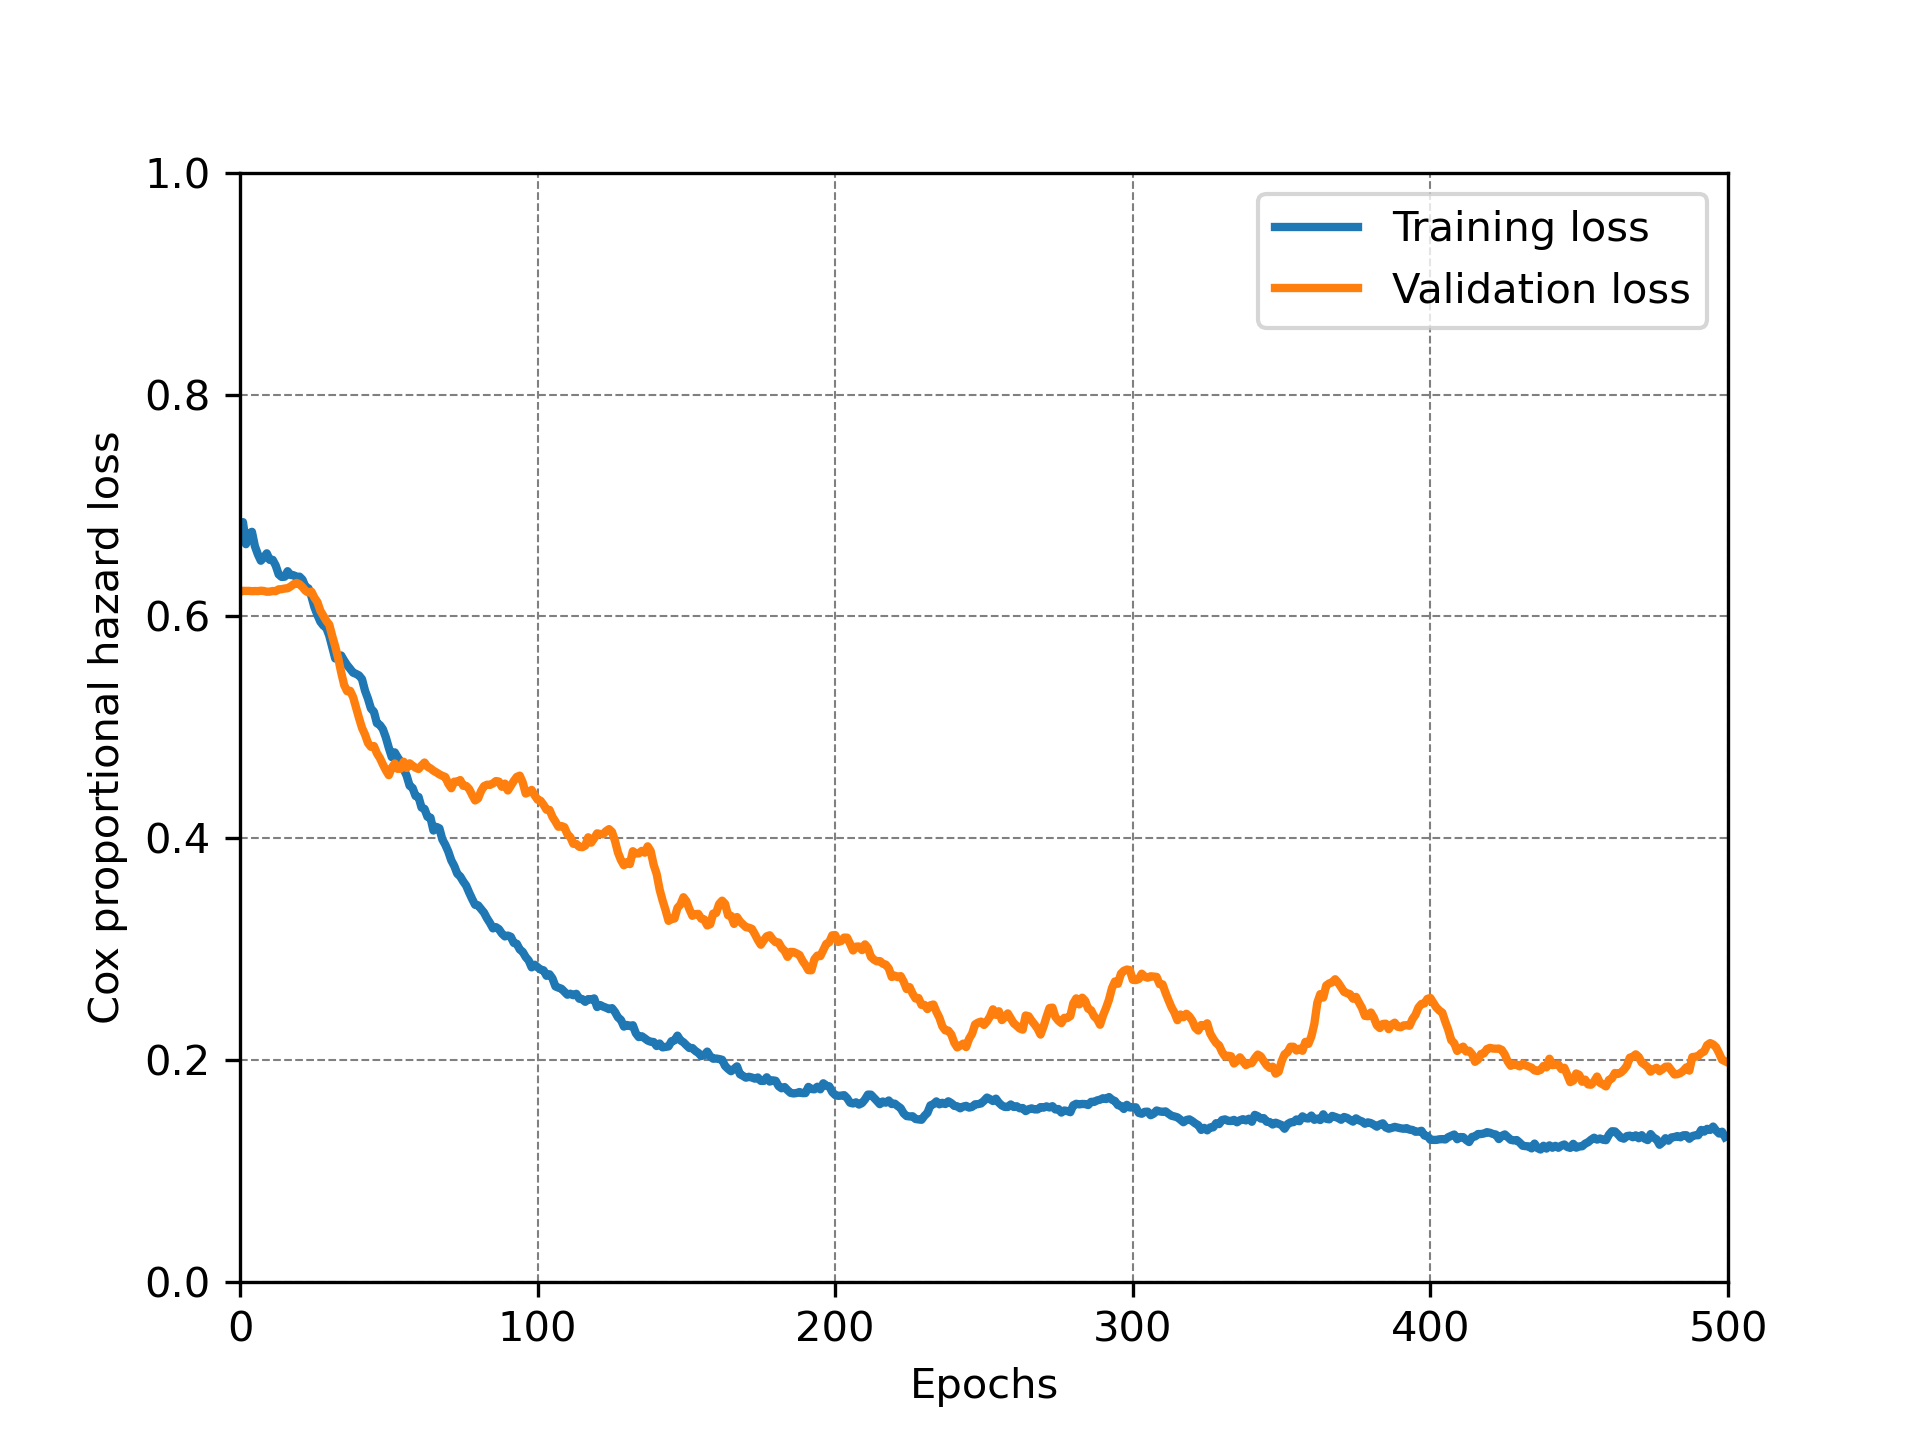
\includegraphics[width=\textwidth]{latex/loss_plots/24accums.png}
     \caption{Losses at 24 gradient accumulations}
    \end{subfigure}
    \hfill
     \begin{subfigure}[b]{0.49\textwidth}
         \centering
         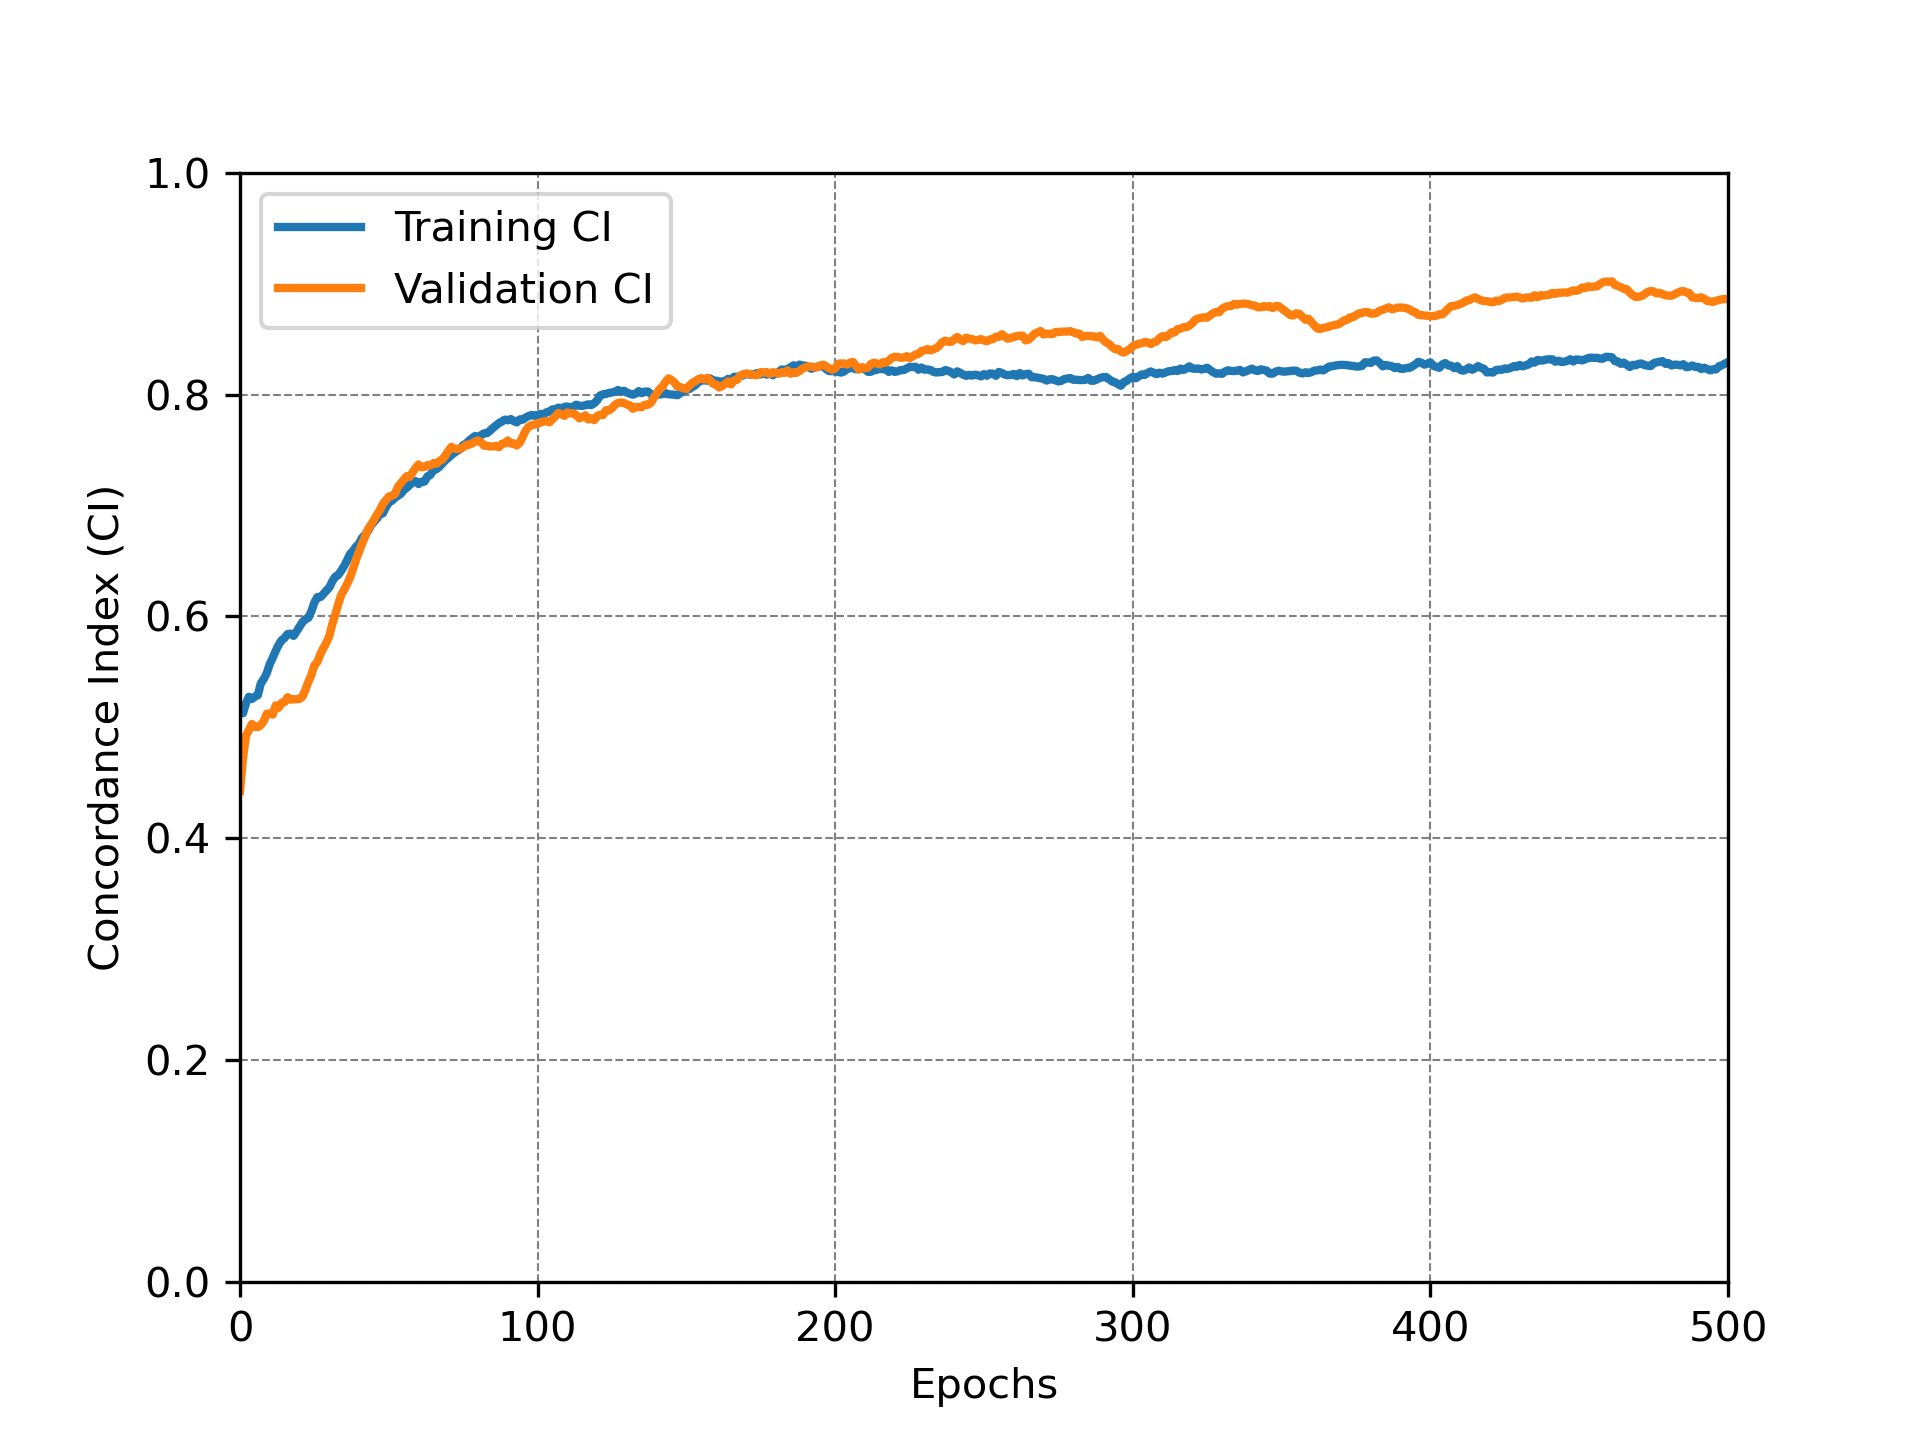
\includegraphics[width=\textwidth]{latex/ci_plots/24accums.png}
         \caption{CI at 24 gradient accumualtions}
     \end{subfigure}
    \hfill
    \caption[Resnet with Double-Layer Prediction ]{ResNet implementation using two fully connected layers for hazard prediction. Comparison of different learning rates (lr) and different number of iterations before an optimisation step.}
    \label{fig:resnet_lr}
\end{figure}

\clearpage

\section{Gene expression data}

\subsection{Quality Control}

Figure \ref{fig:RCCQC} shows the results of the quality controls for the gene expression data. The presented controls were first conducted by NanoString, but then repeated due to concerns regarding quality of the provided data. 
\subsubsection{Binding Density} The binding density of the probes within the imaging area is shown in figure \ref{fig:BindDens} as the concentrations of barcodes per lane. Samples are shown as green dots, and panel standards are shown as green triangles. There are two samples per lane, as two cartridges were used for the experiment. The lower and upper thresholds for passing the control are situated at 0.5 and 2.5 respectively and visualised as grey dashed lines. Most samples have a binding density below that of the standards (at a binding density of about 0.9). The only exception is one sample in lane 7 and both samples from lane 12. All samples pass the control, with the samples in lane 1 barely above the minimum threshold. \cite{Gorman2022IO, NanoStringTechnologies2017Gene}
\subsubsection{Limit of Detection} The limit of detection is shown in figure \ref{fig:LOD}. It represents a comparison of positive and negative controls. The counts of the negative controls are seen as box plots, each having a mean count below 16. The positive control \verb|Pos_E| has a concentration of 0.5 fM. It is required to be at least two standard deviations higher in terms of counts. This threshold is shown as a red horizontal line for each sample, respectively. All samples pass this control as well. Also, all samples have more counts than the panel standards. \cite{Gorman2022IO, NanoStringTechnologies2017Gene}
\subsubsection{Positive Linearity Control} The results of the positive linearity control are illustrated in figure \ref{fig:PosLin}. It shows the positive controls and the panel standards, which have different target concentrations. Corresponding data points are connected by edges. The correlation after $Log_2$ transformation between the known concentrations of positive controls and the observed counts is shown. Correlations below 0.95 may indicate problems. However, all samples pass this control as well. \cite{Gorman2022IO, NanoStringTechnologies2017Gene}

\begin{figure}[h!t]
    \centering
 \begin{subfigure}[b]{0.475\textwidth}
     \centering
     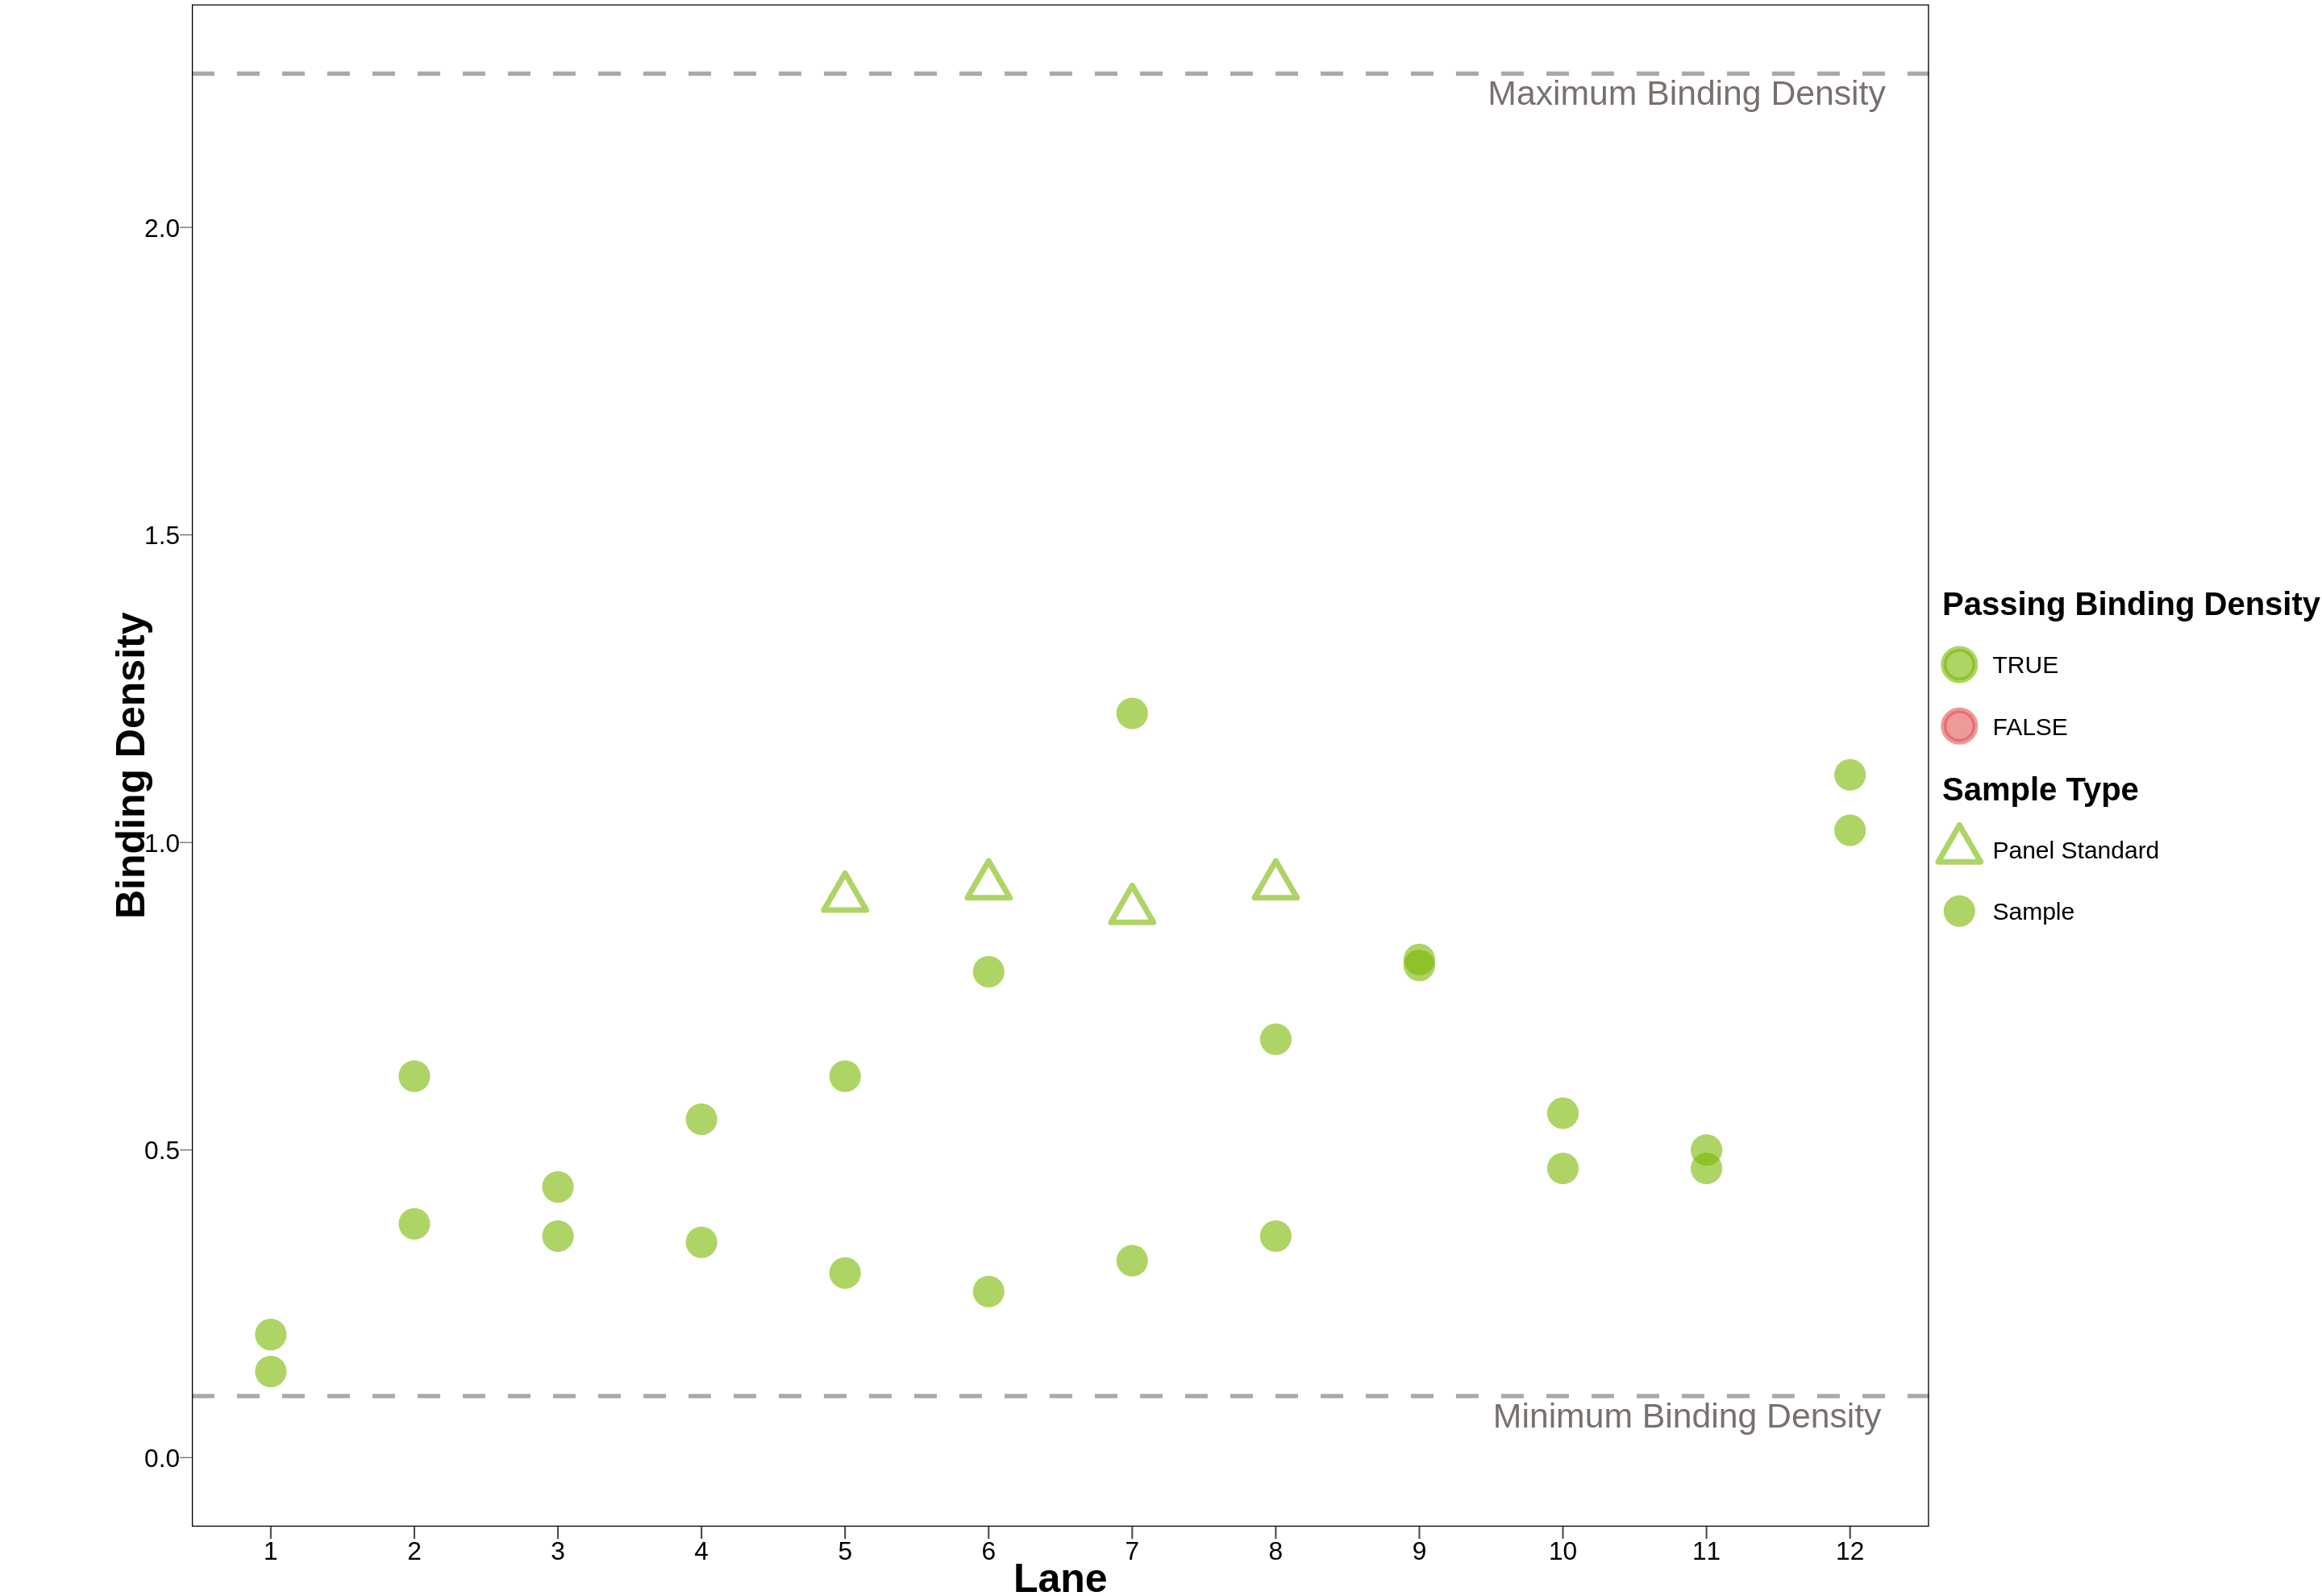
\includegraphics[width=\textwidth]{latex/figures/NanostringBindingDensity.png}
     \caption{Binding Density}
     \label{fig:BindDens}
 \end{subfigure}
    \hfill
     \begin{subfigure}[b]{0.475\textwidth}
         \centering
         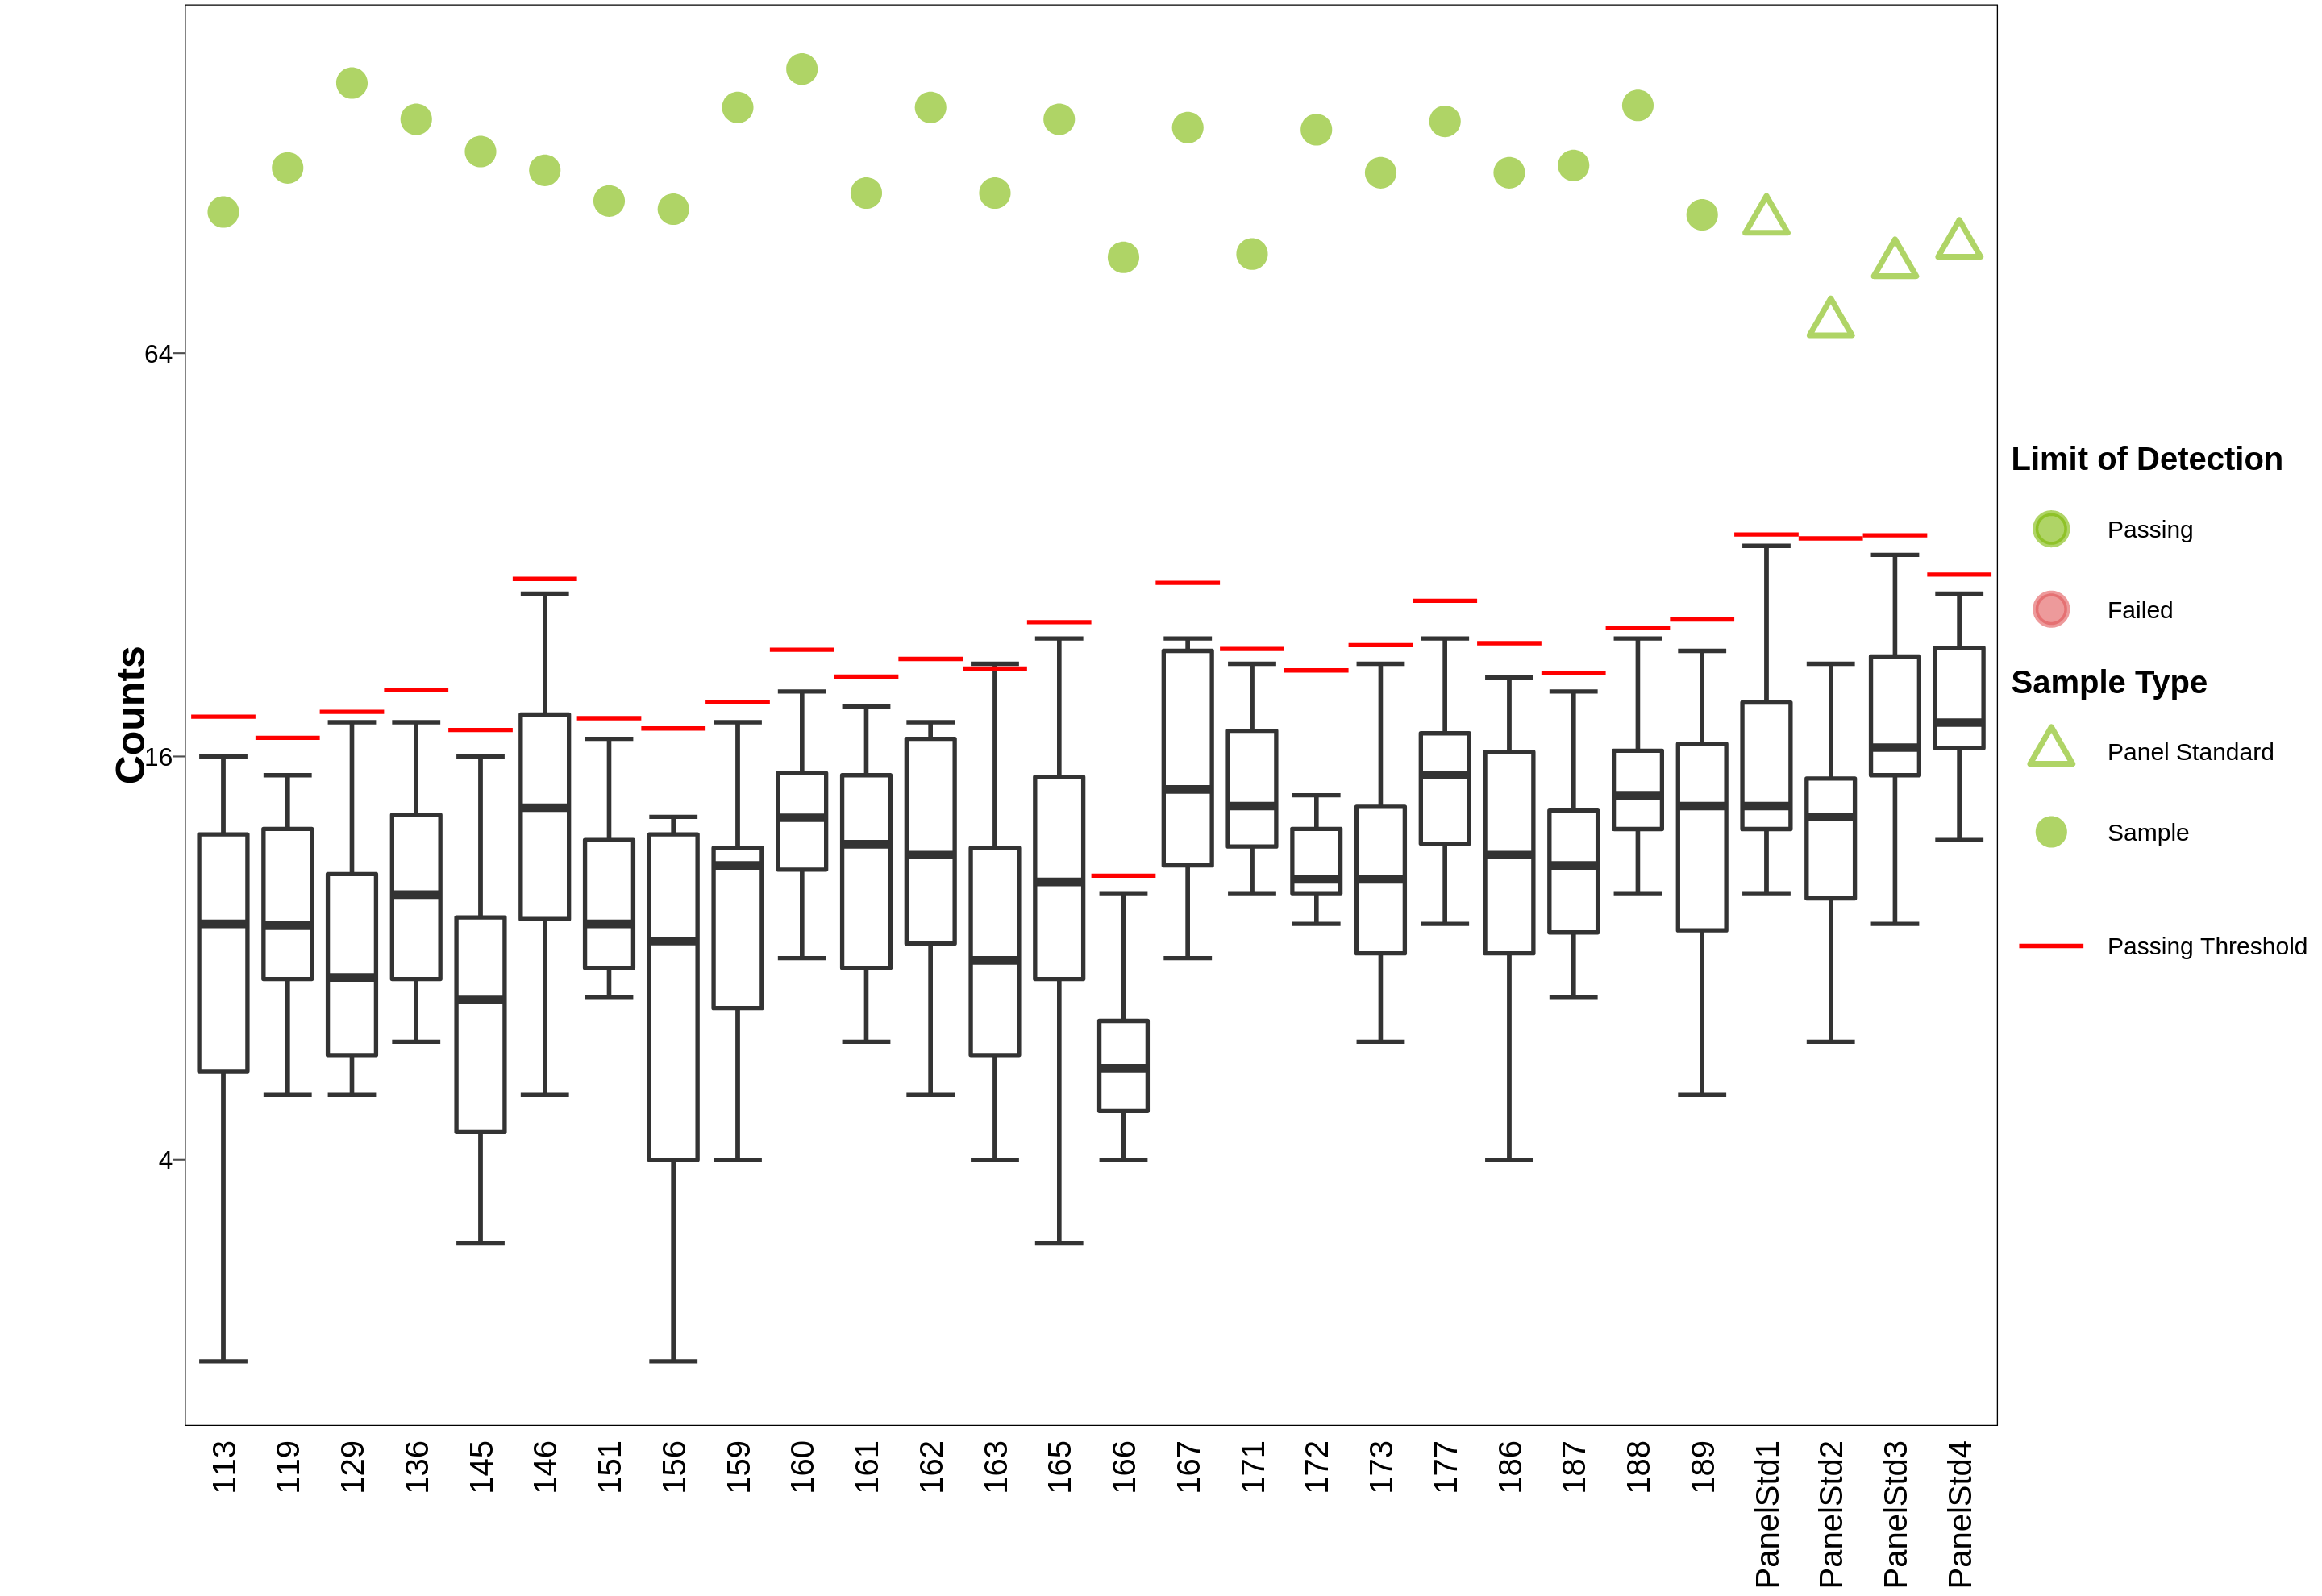
\includegraphics[width=\textwidth]{latex/figures/PositiveLimitOfDetection.png}
         \caption{Limit of Detection}
         \label{fig:LOD}
     \end{subfigure}
    \vskip\baselineskip
     \begin{subfigure}[b]{0.475\textwidth}
         \centering
         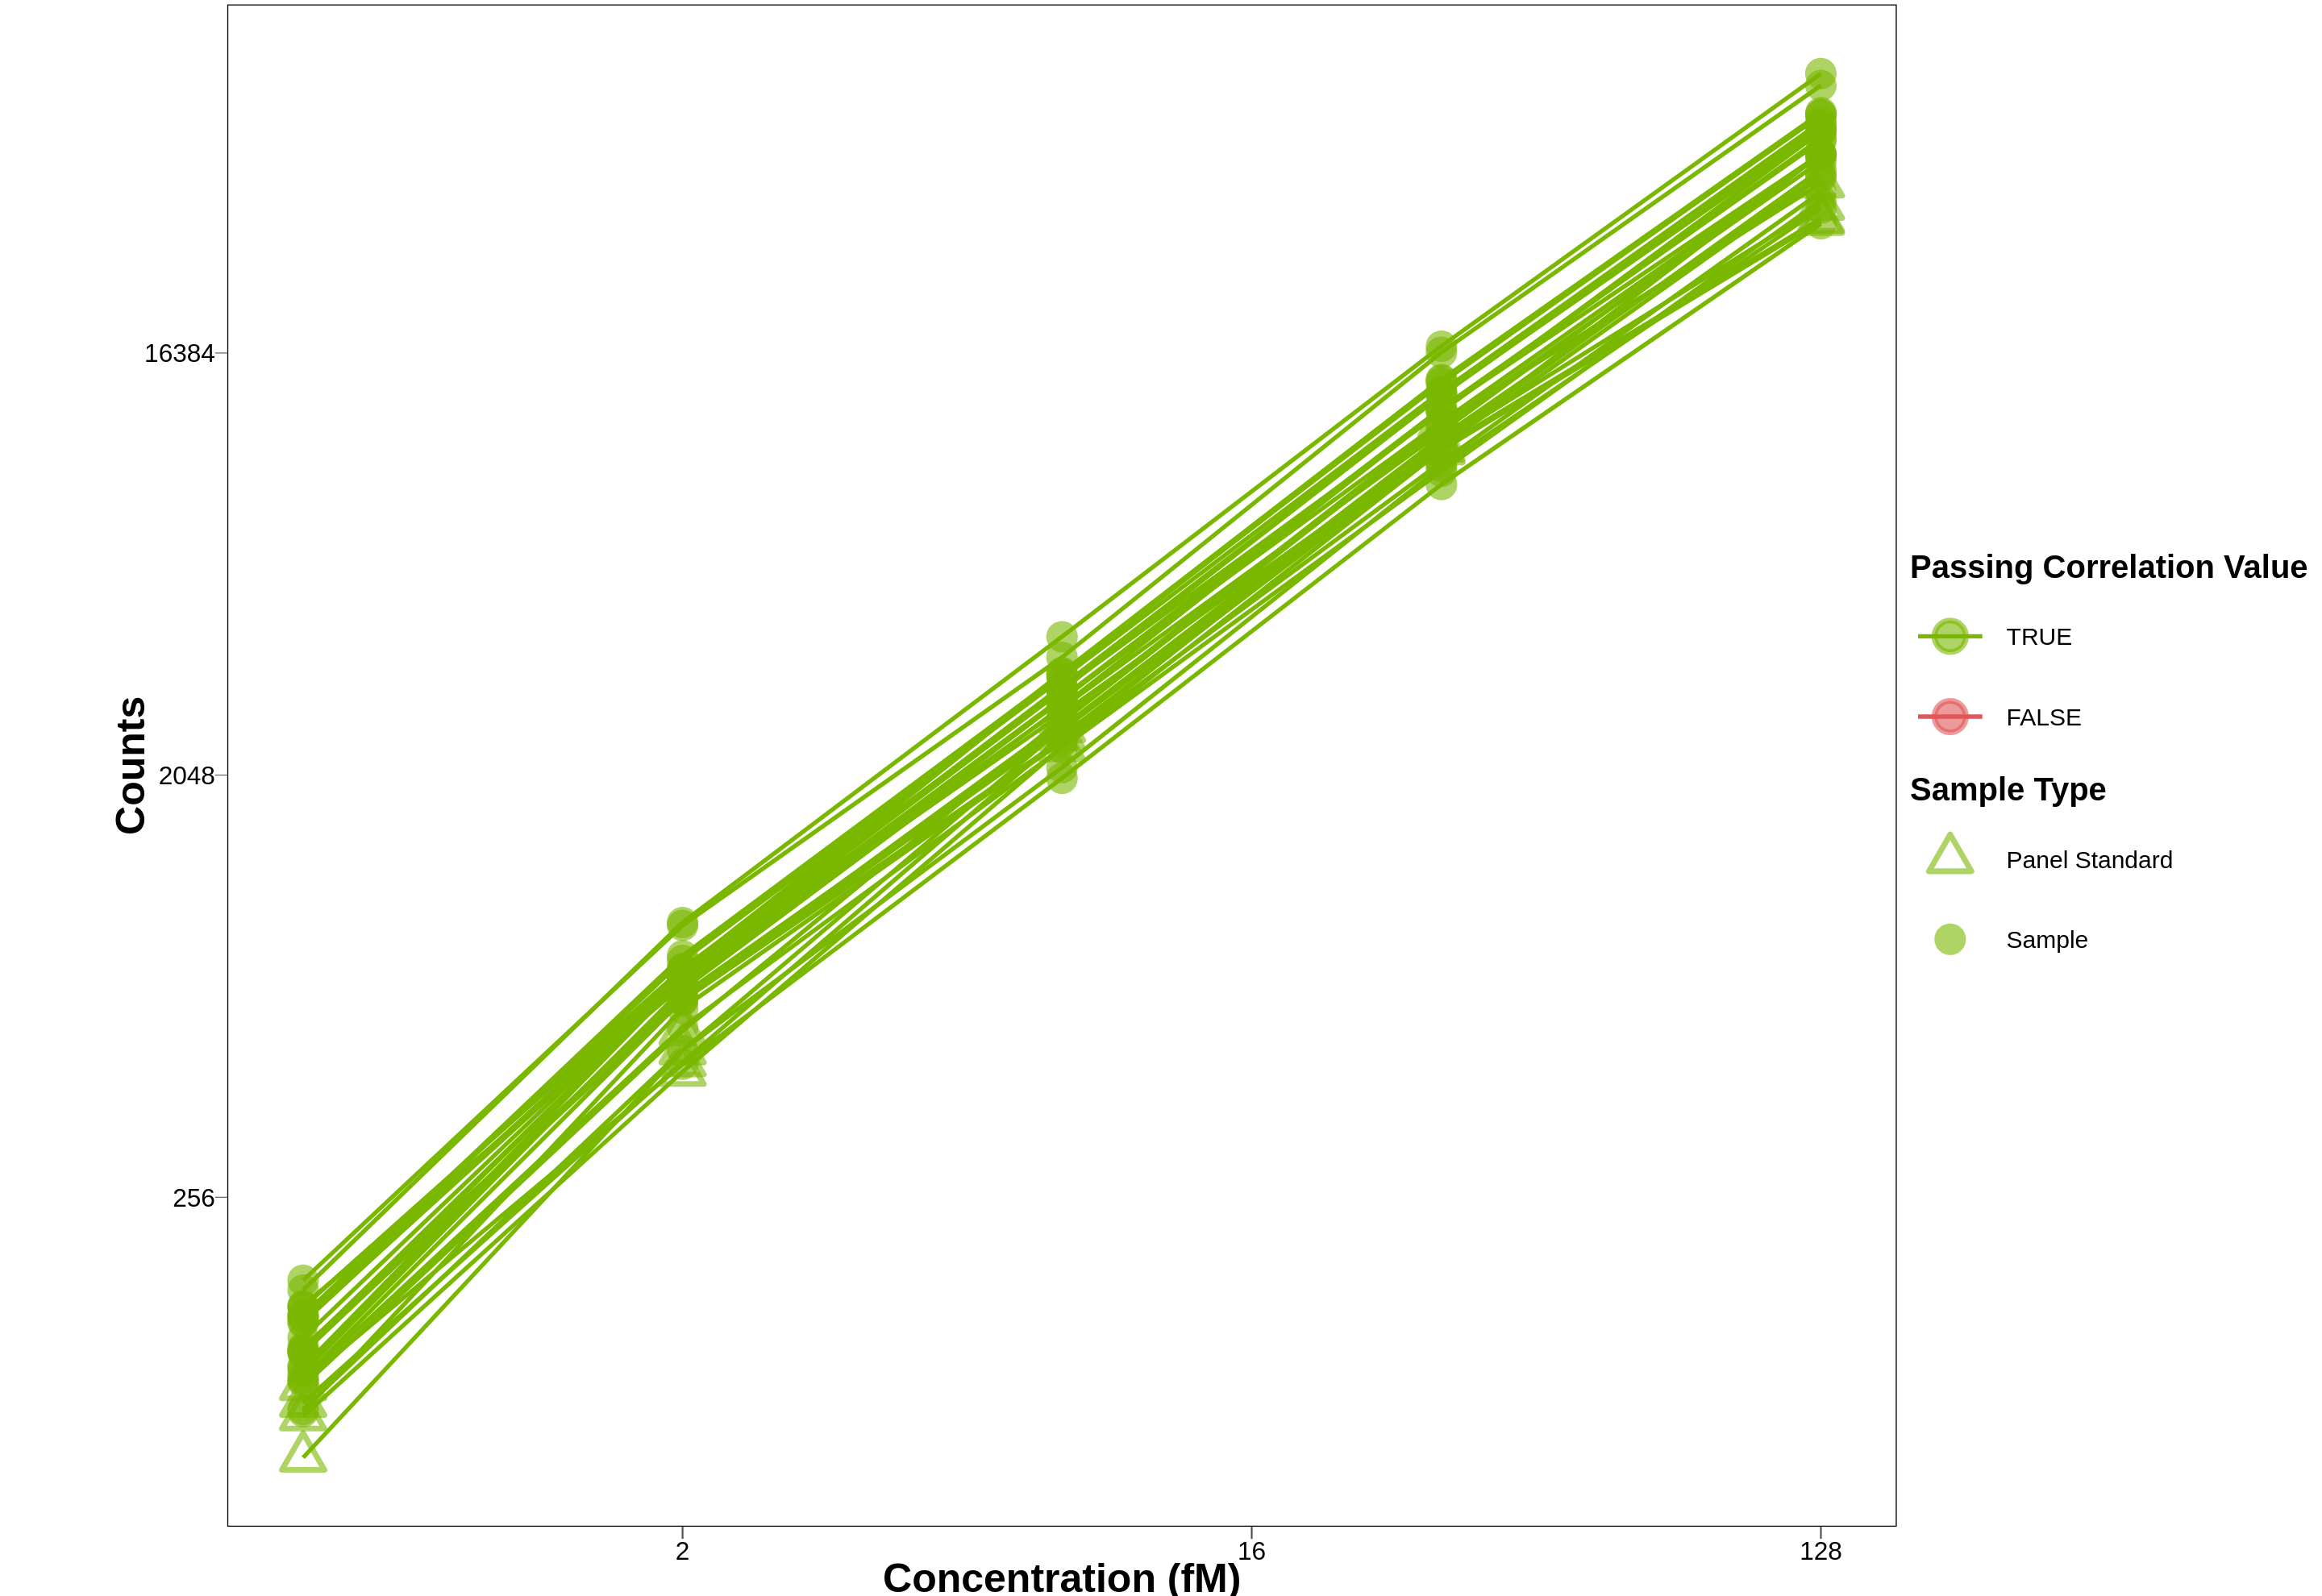
\includegraphics[width=\textwidth]{latex/figures/PositiveLinearity.png}
         \caption{Positive Linearity}
         \label{fig:PosLin}
     \end{subfigure}
    \hfill
    \caption[NanoString Quality Control]{Visualisations of Quality Control metrics. Figure \ref{fig:BindDens} shows the binding density of each sample respective to their lane as green dots. Dashed grey lines show the respective upper and lower thresholds, while green triangles represent the panel standards for comparison. Figure \ref{fig:LOD} shows the limit of detection as counts per sample and of the panel standards. The box plots correspond to the negative controls. Red horizontal lines represent the threshold each sample has to pass. Figure \ref{fig:PosLin} shows the positive control linearity. For each sample, the counts of the respective positive controls and the panel standards are shown against the concentration in femtomolar (fM). 
    Each sample passes all quality controls. Each figure were taken from the automated report conducted by NanoString \cite{Gorman2022IO}} 
    \label{fig:RCCQC}
\end{figure}


\subsection{Baseline model}

A Baseline model was fitted to the subcohort of 24 samples for which gene expression data was available. This model achieved a concordance index of $0.98$ and $1.0$ on train and test data, respectively.
Figure \ref{fig:SurvRaceSmall} gives an overview over the available data. Of 24 patients, 14 are censored, leaving 10 patients with recorded survival times. Most uncensored patients showed a relatively short survival time, with patient 151 being a notable exception. An identical Figure for the whole cohort can be found in the appendix (Figure \ref{fig:SurvRaceFull}).
For each of the 750 cancer-relevant genes, the model did calculate the hazard ratios (HR) as log-transformed coefficients. Figure \ref{fig:HRGenes} shows the subset of genes with $log(\text{HR})$ of less than $0.99$ or more than $1.01$. These genes have a particularly positive or negative effect on patient survival.
Figure \ref{fig:DevianceResiduals} visualises the deviance residuals of patients and their survival times. Except for one value, all samples are situated in the range of $[-1,1]$. Censored and uncensored patients are marked blue and orange, respectively.

\begin{figure}[h!t]
    \centering

     \begin{subfigure}[b]{0.49\textwidth}
         \centering
         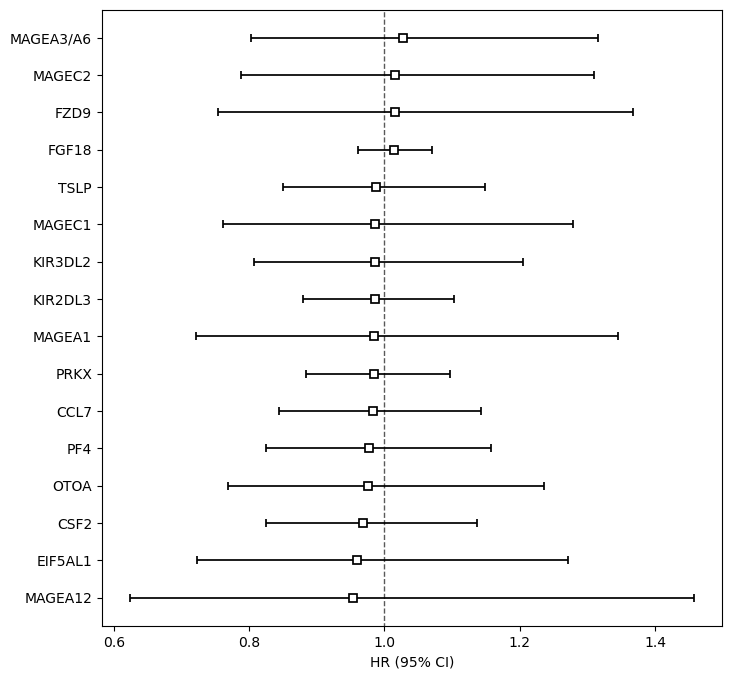
\includegraphics[width=\textwidth]{latex/figures/impactful_genes_hazard_ratio.png}
         \caption{Features with HR $\ge 1.01$ or $\le 0.99$}
         \label{fig:HRGenes}
     \end{subfigure}
    \hfill
     \begin{subfigure}[b]{0.49\textwidth}
         \centering
         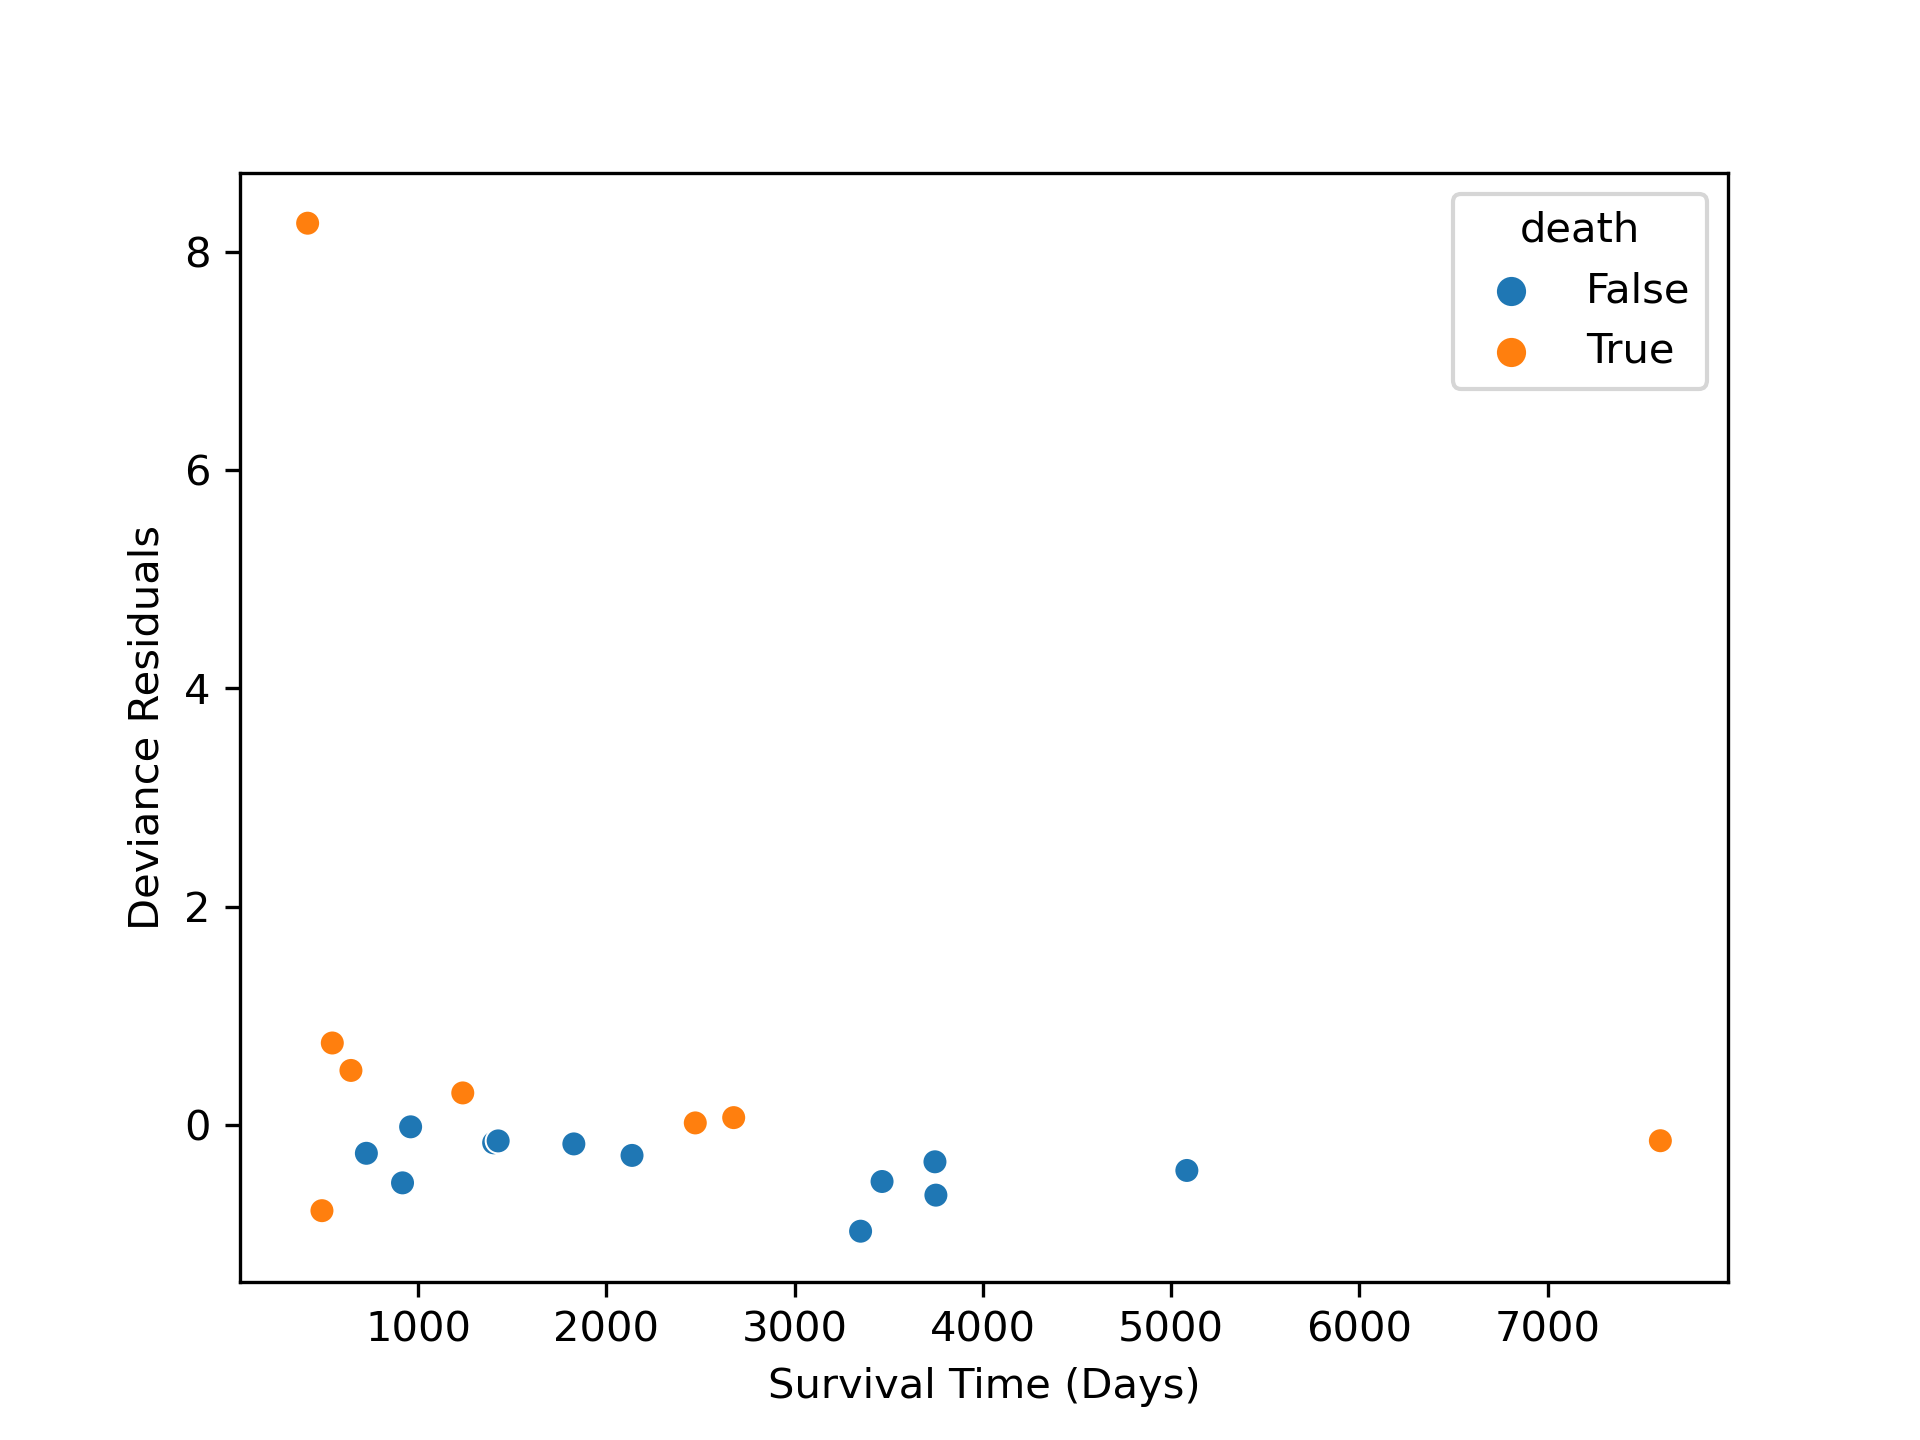
\includegraphics[width=\textwidth]{latex/figures/deviance_residuals_rcc.png}
         \caption{Deviance Residuals}
         \label{fig:DevianceResiduals}
     \end{subfigure}

    \hfill
    \caption[Baseline model on genomic data]{
    Figure \ref{fig:HRGenes} shows genes with notable hazard ratios (HR) and their respective error bars.
    Figure \ref{fig:DevianceResiduals} shows the deviance residuals per patient over their survival times. Censoring status is marked as orange or blue if the patient died or got censored, respectively.}
    \label{fig:BaselineModel}
\end{figure}

\subsection{Self normalising Neural networks}

Figures \ref{fig:snn_dropout} and \ref{fig:snn_fsz} show the hyperparameter search experiments for the SNN trained on gene expression data. After a preliminary search for a suitable learning rate, with the result being \(1e-5\), we explored different dropout probabilities as well as output sizes for the feature extraction part of the network. Due to strong fluctuations in values between consecutive epochs, exponential moving averaging was applied to all results with a window size of 30. 

Figure \ref{fig:snn_dropout} shows the result for varying probabilities for randomly dropping single nodes in each hidden layer. We note that both the concordance index and the loss stagnate with a dropout ratio of 0.5. The only exception is the validation loss, where a steady rise is observed. Generally, when looking at the metrics during training, we can observe that a lower dropout probability results in a more convex loss and CI over time. 
When inspecting the validation data, we notice that the loss increases until a certain plateau is hit, after which it decreases for some epochs before it starts to rise again. Meanwhile, a lower value for $p$ seems to help the CI rise earlier for the validation set. However, there does not seem to be a notable difference for the final (smoothed) values.

\begin{figure}[h!t]
    \centering
 \begin{subfigure}[b]{0.49\textwidth}
     \centering
     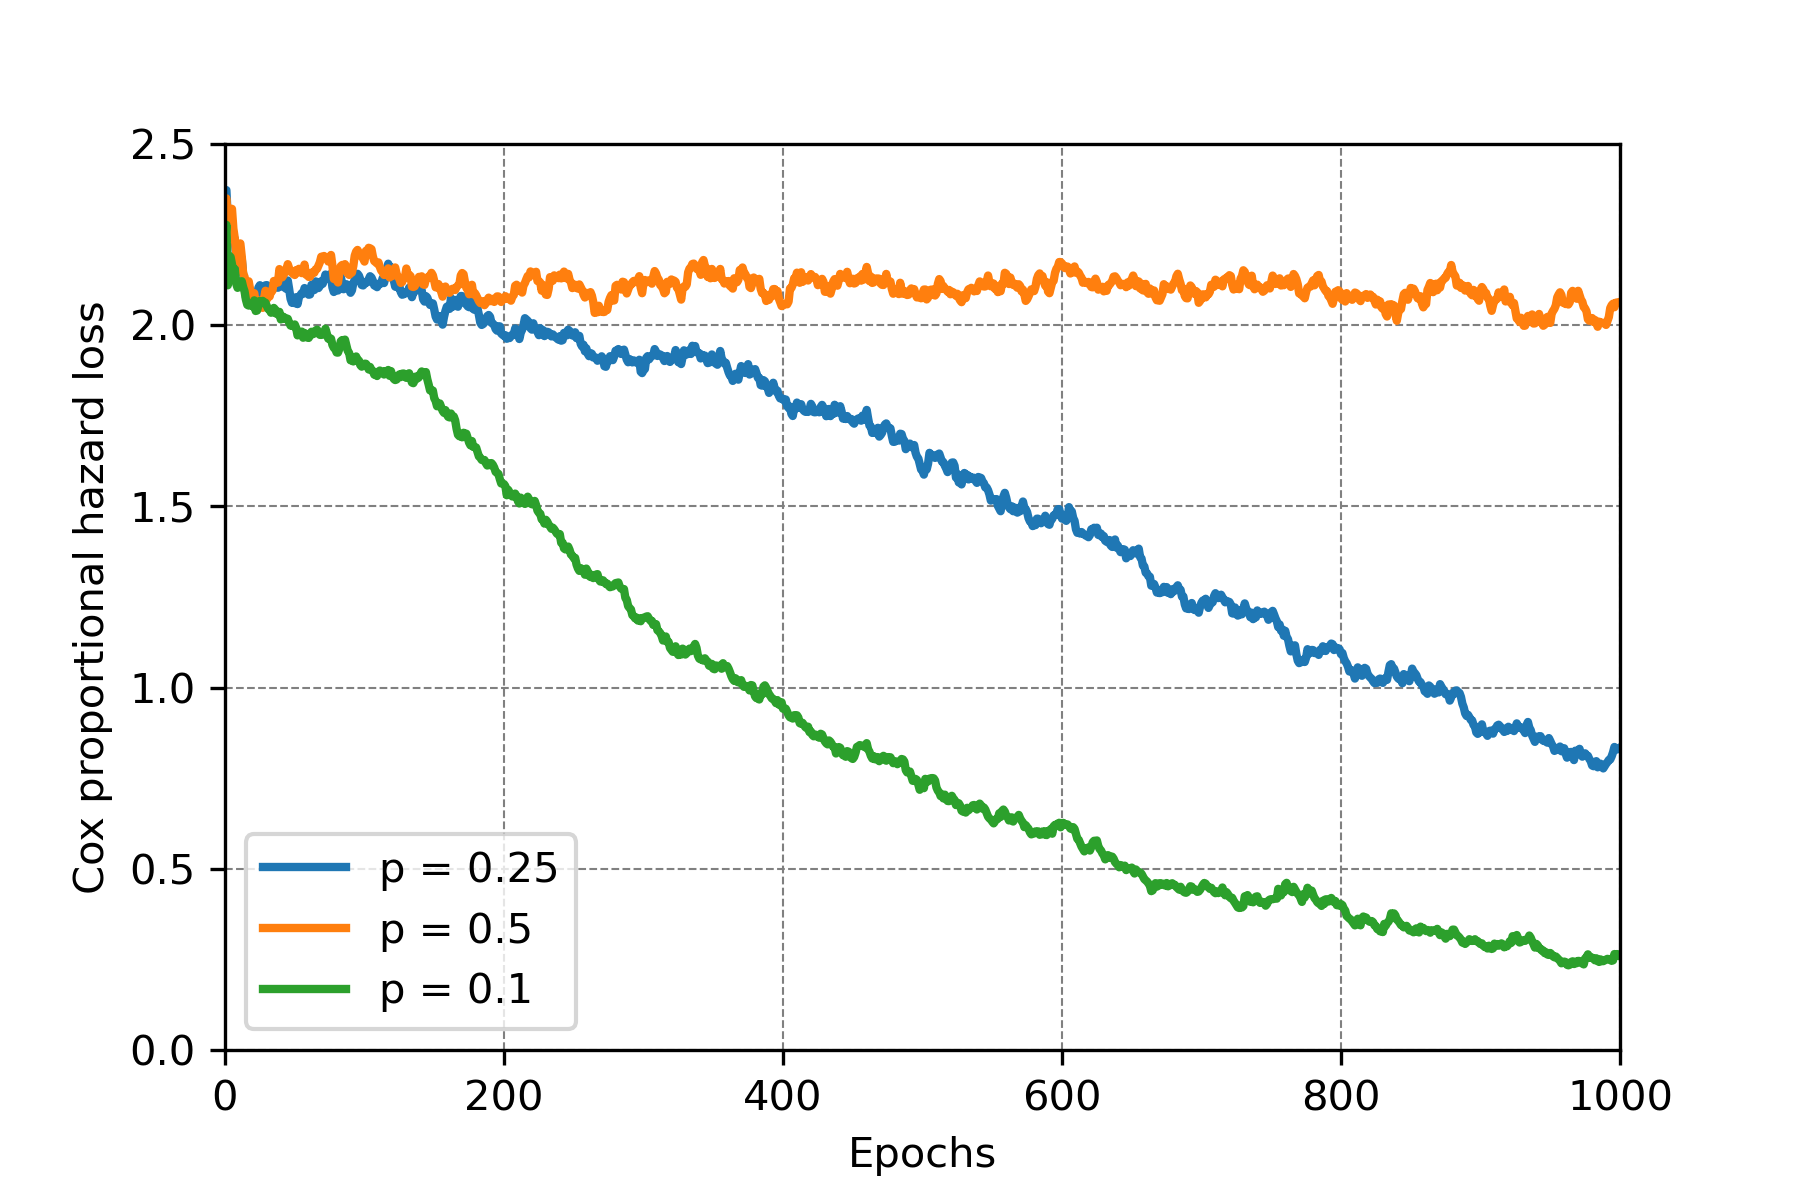
\includegraphics[width=\textwidth]{latex/loss_plots/snn_dropout_train.png}
     \caption{Training loss}
 \end{subfigure}
    \hfill
     \begin{subfigure}[b]{0.49\textwidth}
         \centering
         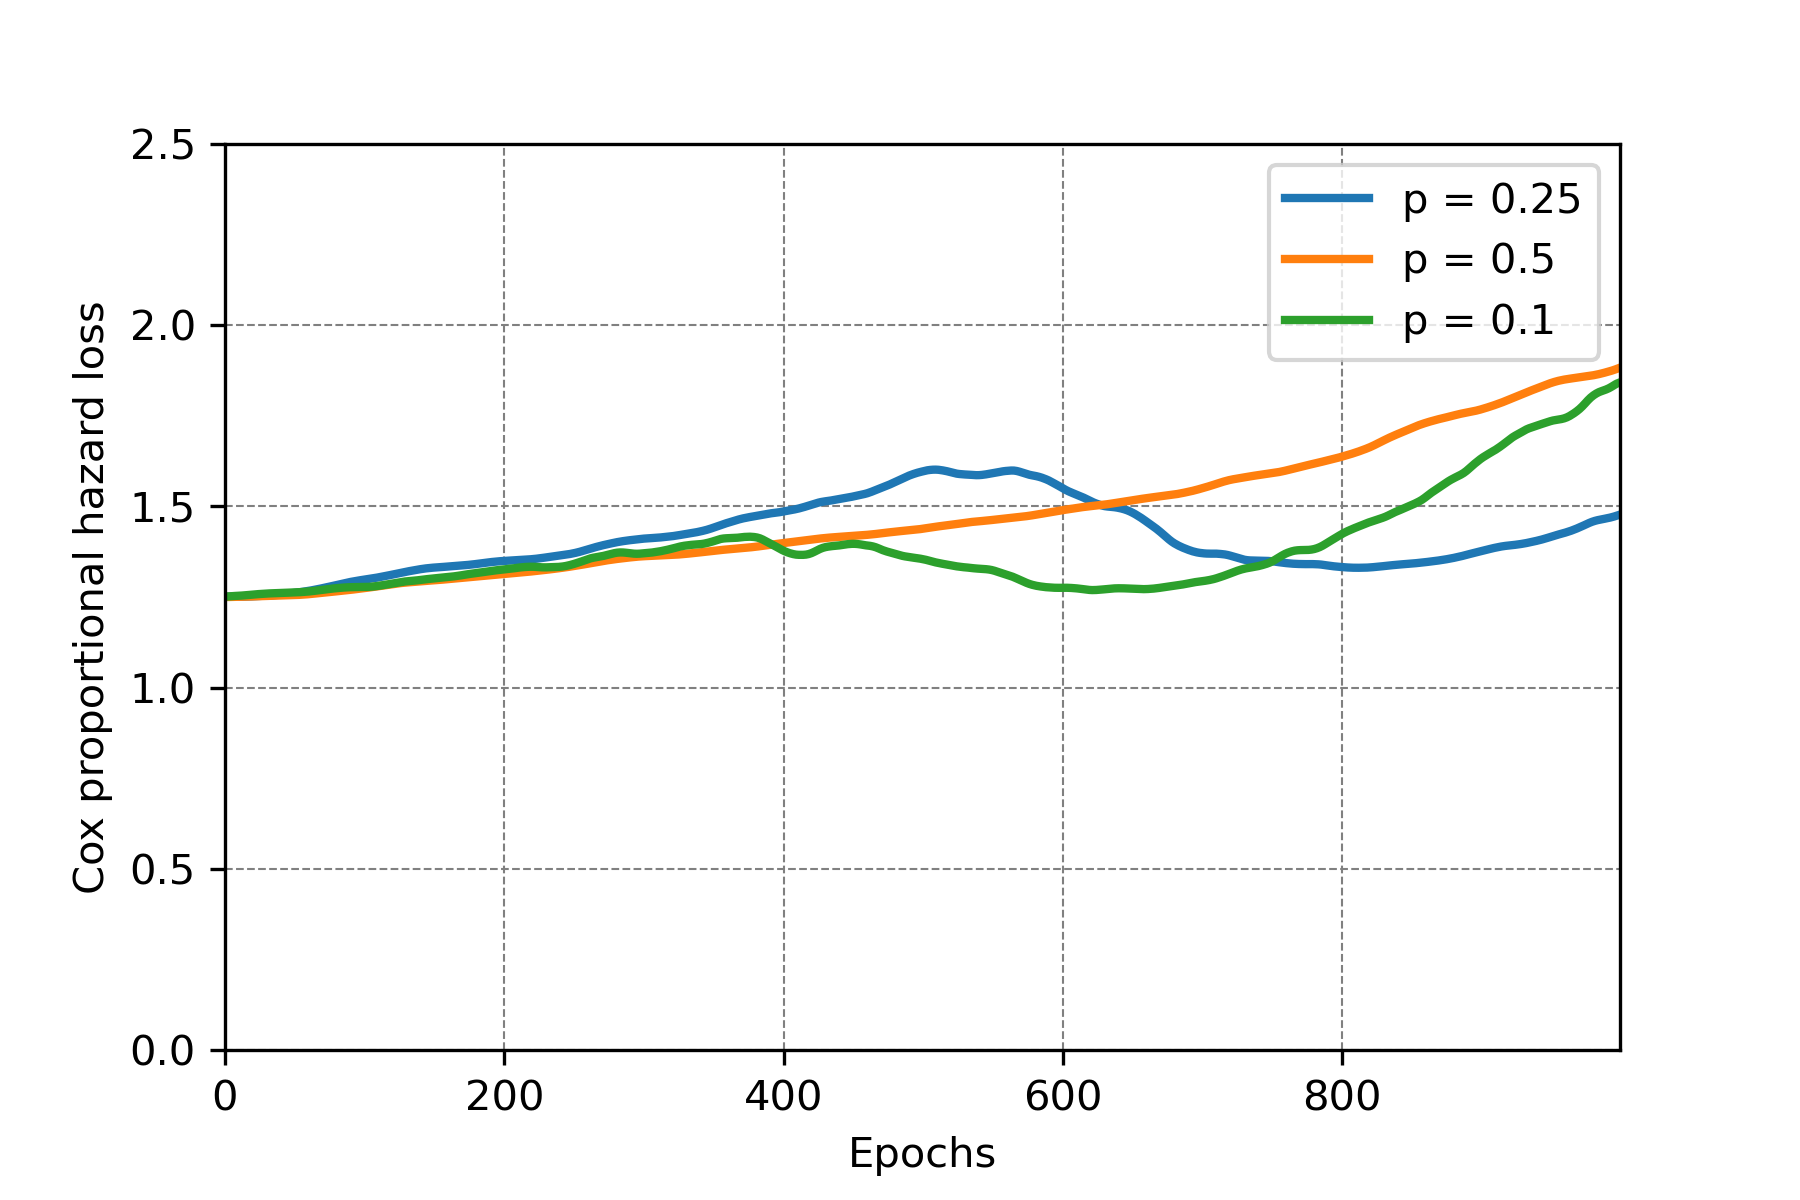
\includegraphics[width=\textwidth]{latex/loss_plots/snn_dropout_val.png}
         \caption{Validation loss}
     \end{subfigure}
\vskip\baselineskip
     \begin{subfigure}[b]{0.49\textwidth}
         \centering
         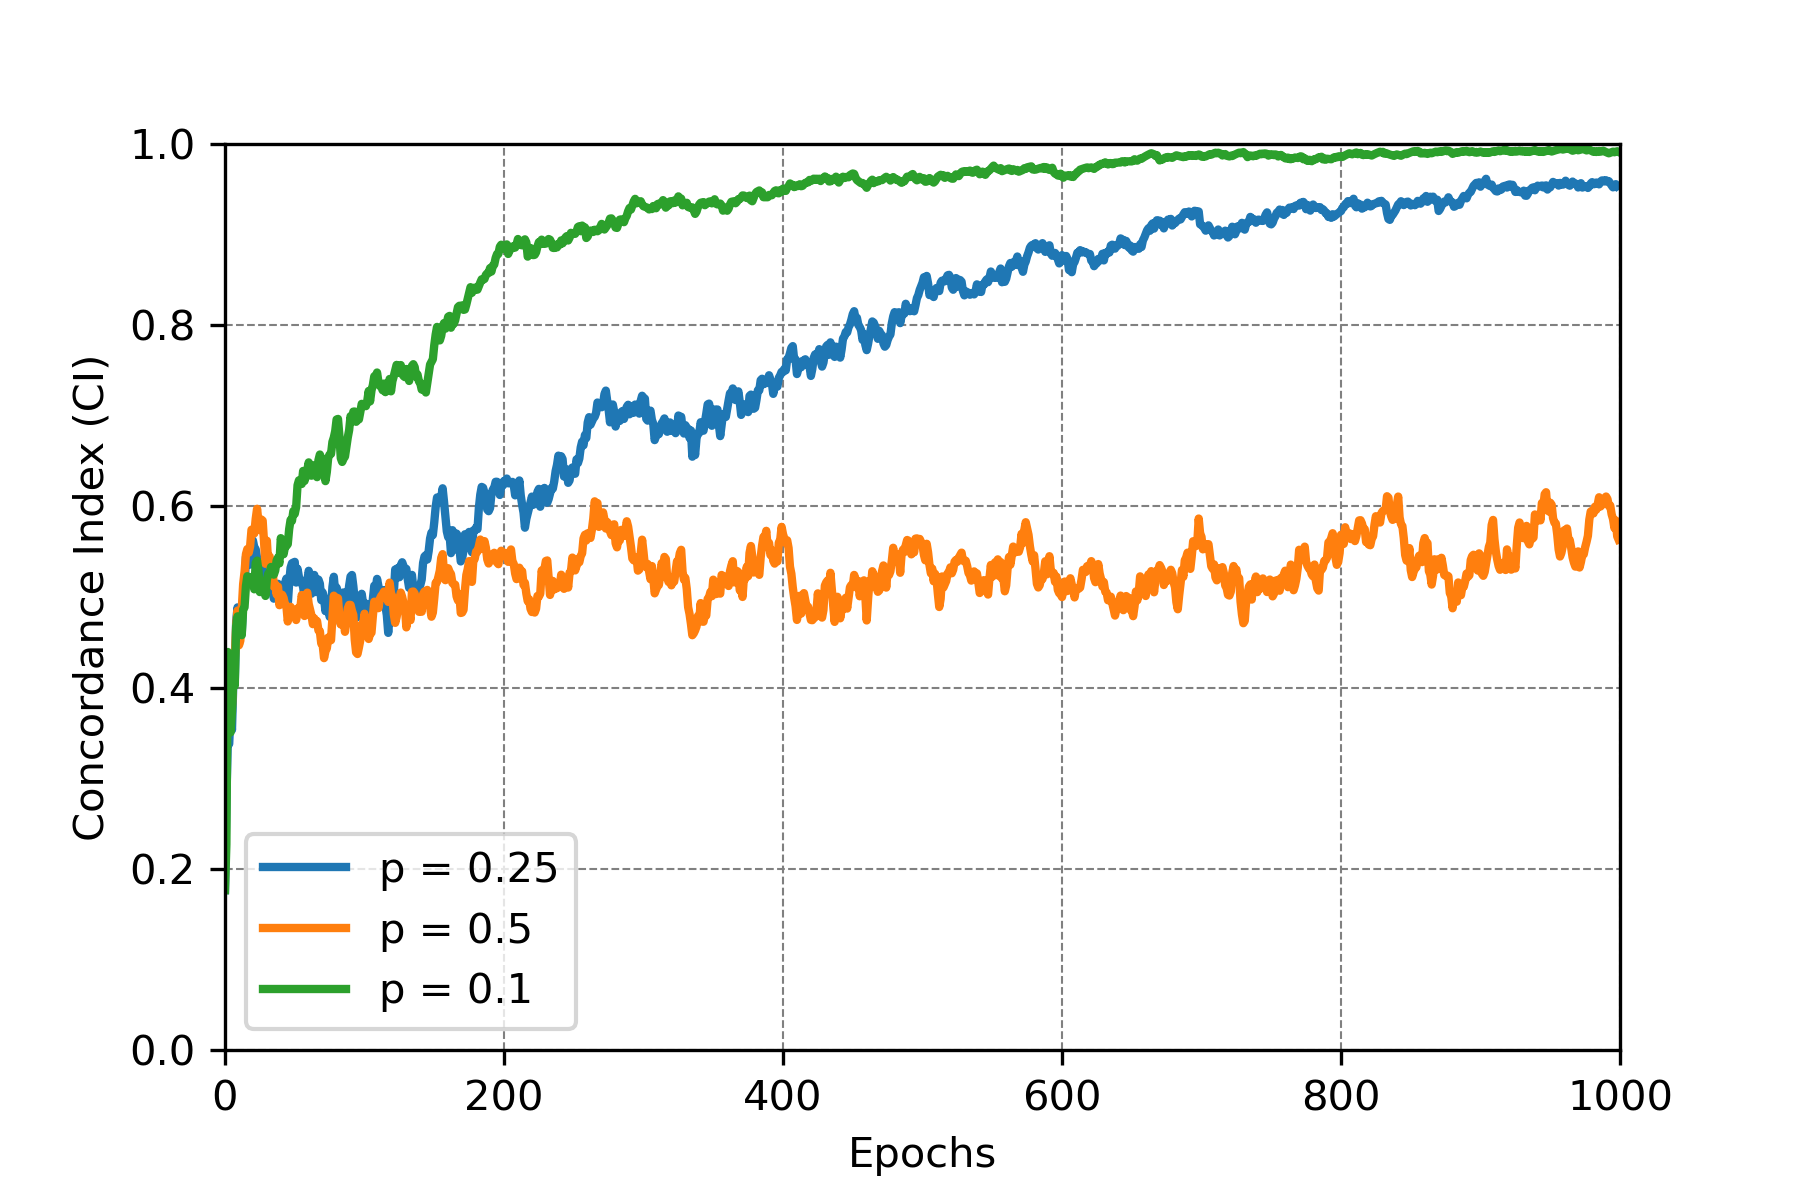
\includegraphics[width=\textwidth]{latex/ci_plots/snn_dropout_train_ci.png}
         \caption{Training concordance index}
     \end{subfigure}
    \hfill
     \begin{subfigure}[b]{0.49\textwidth}
         \centering
         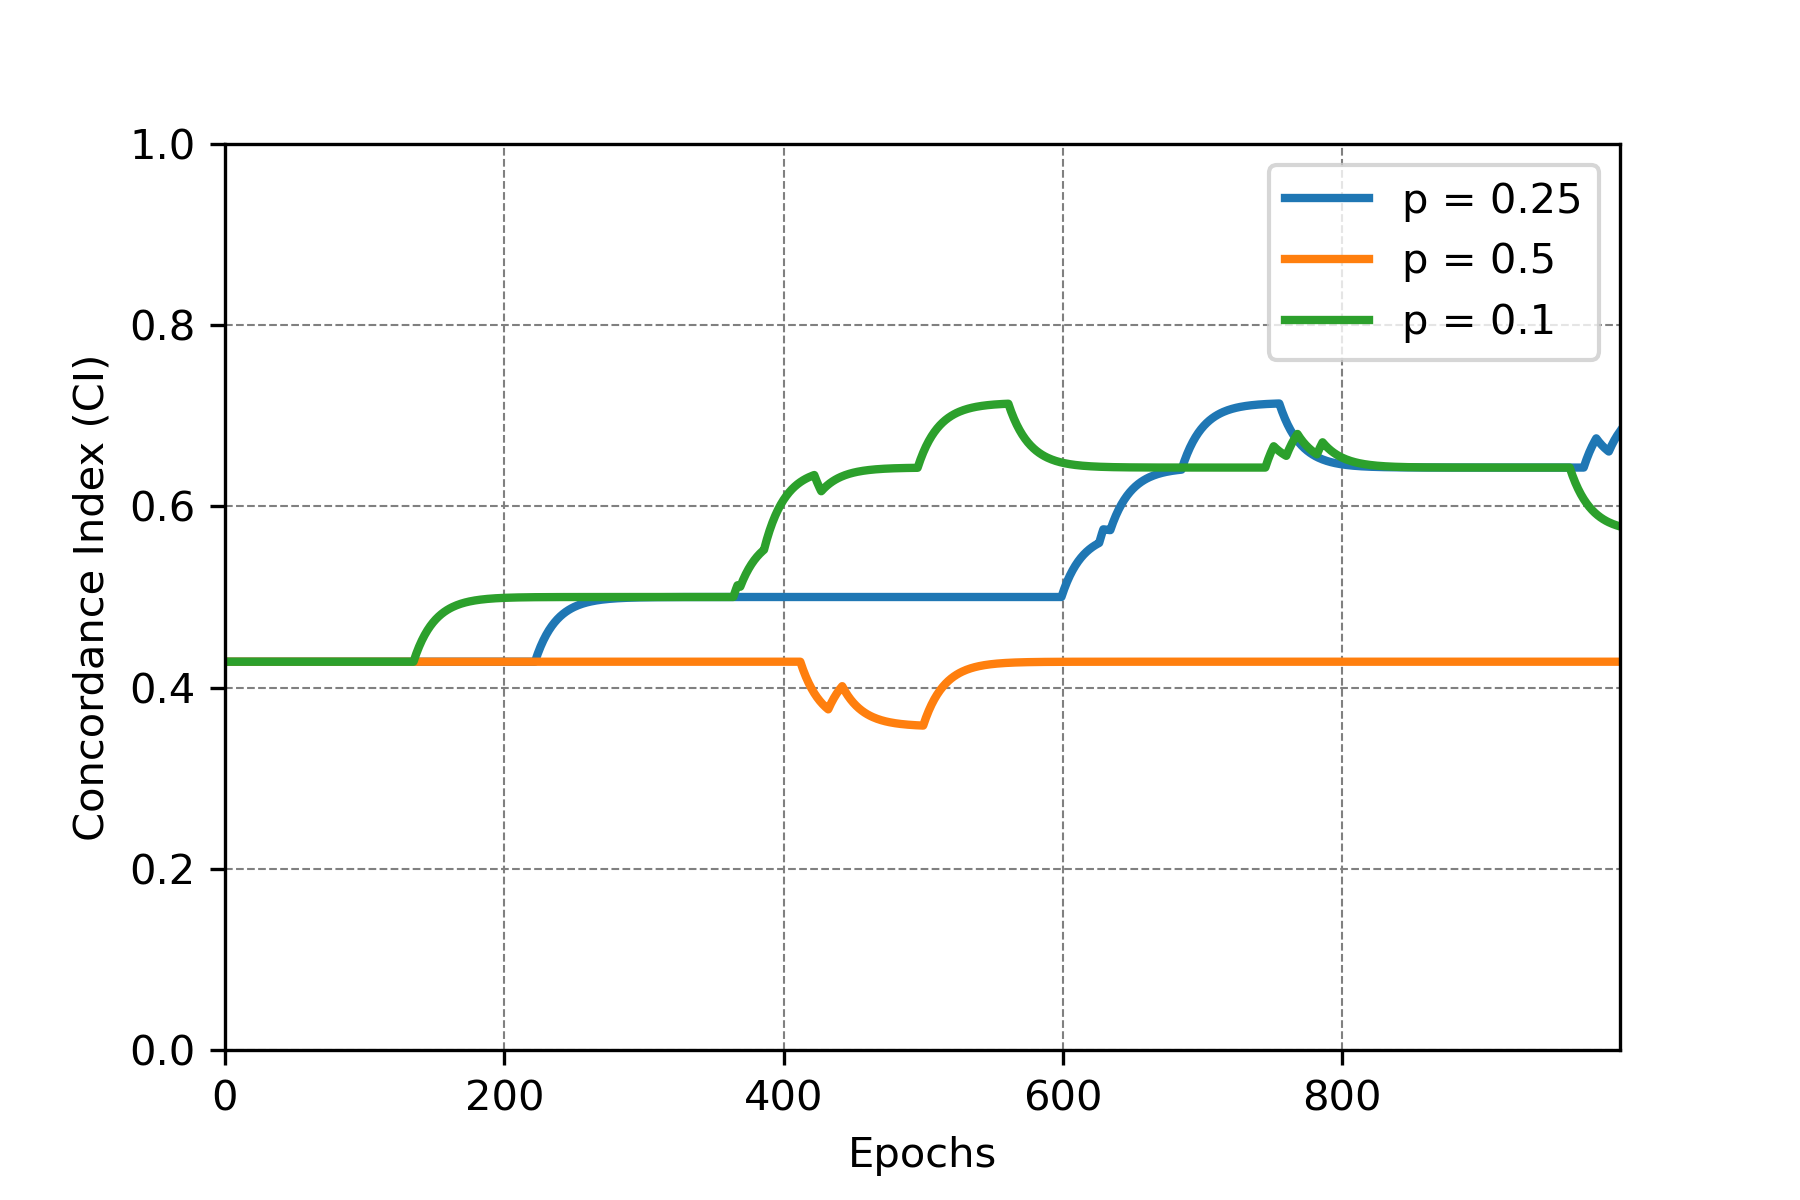
\includegraphics[width=\textwidth]{latex/ci_plots/snn_dropout_val_ci.png}
         \caption{Validation concordance index}
     \end{subfigure}
    \hfill
    \caption[Experiments on dropout probability for SNN]{Experiments on dropout probability for SNN. All parameters of the network stayed the same, except for the probability parameter of each alpha dropout layer in the network. All models were trained for the same duration on the same hardware. Each curve was smoothed using exponential moving averages with a window of 30 samples.}
    \label{fig:snn_dropout}
\end{figure}

Figure \ref{fig:snn_fsz} illustrates the behaviour of the metrics dependent on the output size in the last hidden layer. We tested four different values by incrementing them by 250 for each experiment. For both the training loss and the training CI, the values differ barely over time. Towards the end of each experiment, the losses are diverging, while the CI values are converging. The differences are less nuanced for the validation dataset. A feature size of 750 resulted in the highest loss over the whole duration of the experiment. The other tested sizes show similar values for the most time until the last 200 epochs, where the smallest size results in the lowest final loss. Generally, the same behaviour as in the experiments related to the dropout rate can be observed. First the loss increases, then a local minimum is found which is left towards the end of the training time. 
The concordance indices for the validation data reflect the inverse results of the loss curves. The lowest feature size achieves the highest CI, while the opposite is the case for the feature size of 750.

\begin{figure}[h!t]
    \centering
 \begin{subfigure}[b]{0.49\textwidth}
     \centering
     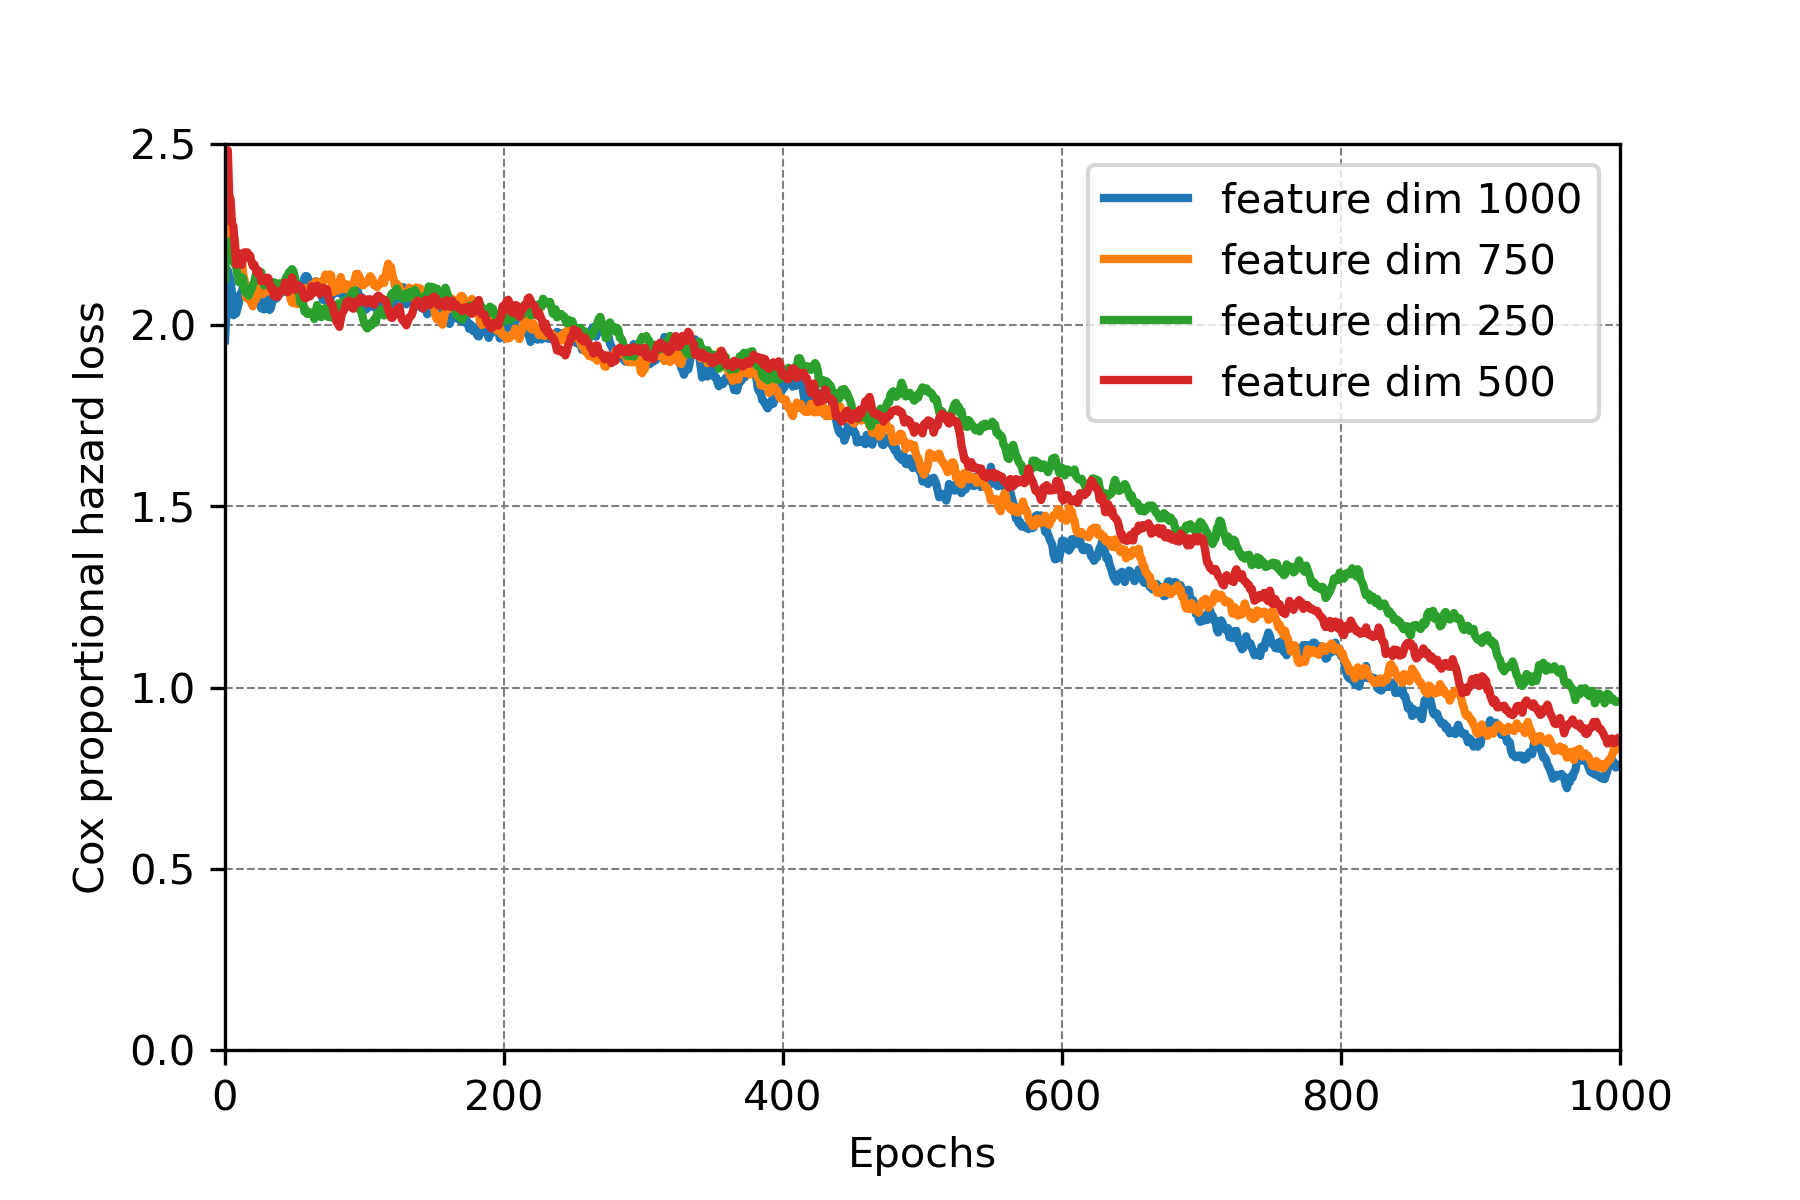
\includegraphics[width=\textwidth]{latex/loss_plots/snn_fsz_train.png}
     \caption{Training loss}
 \end{subfigure}
    \hfill
     \begin{subfigure}[b]{0.49\textwidth}
         \centering  
         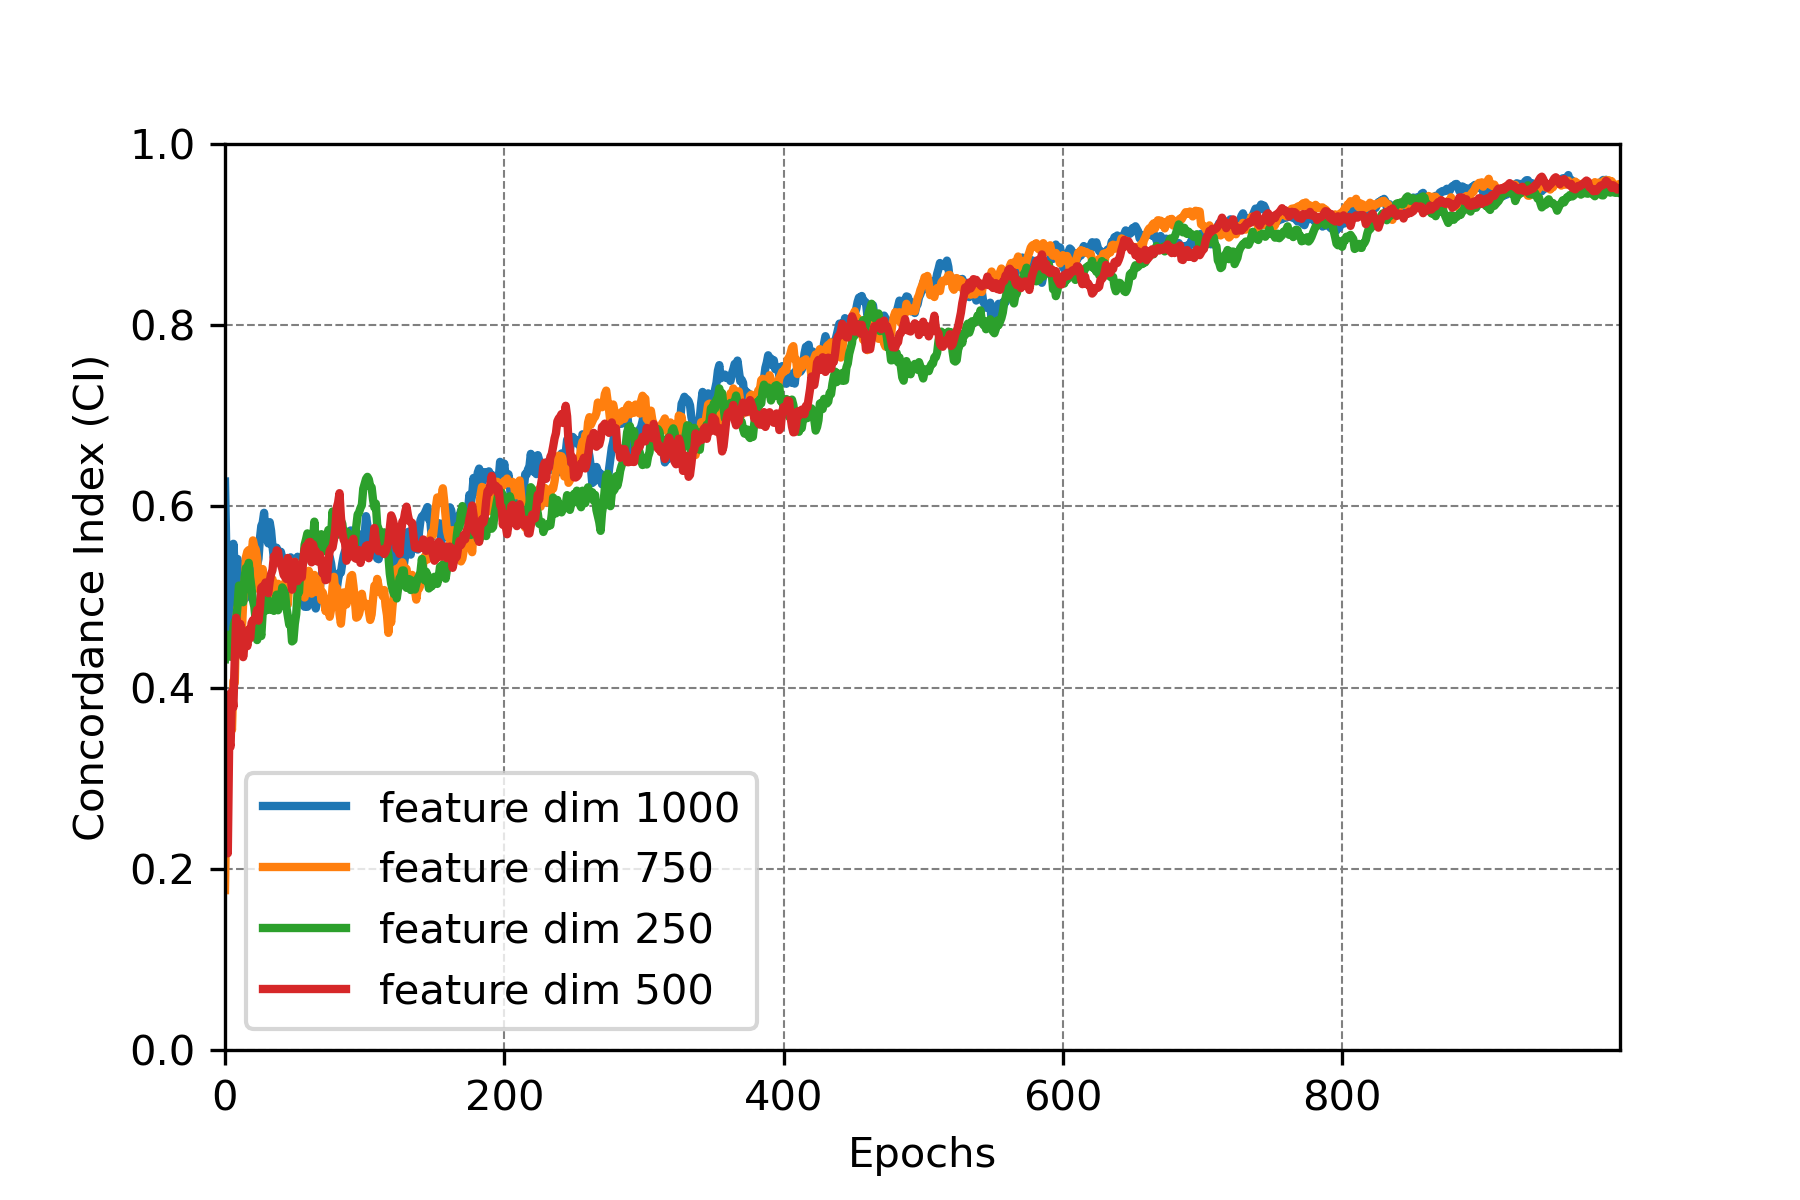
\includegraphics[width=\textwidth]{latex/ci_plots/snn_fsz_train_ci.png}
         \caption{Training concordance index}
     \end{subfigure}
\vskip\baselineskip
     \begin{subfigure}[b]{0.49\textwidth}
         \centering
         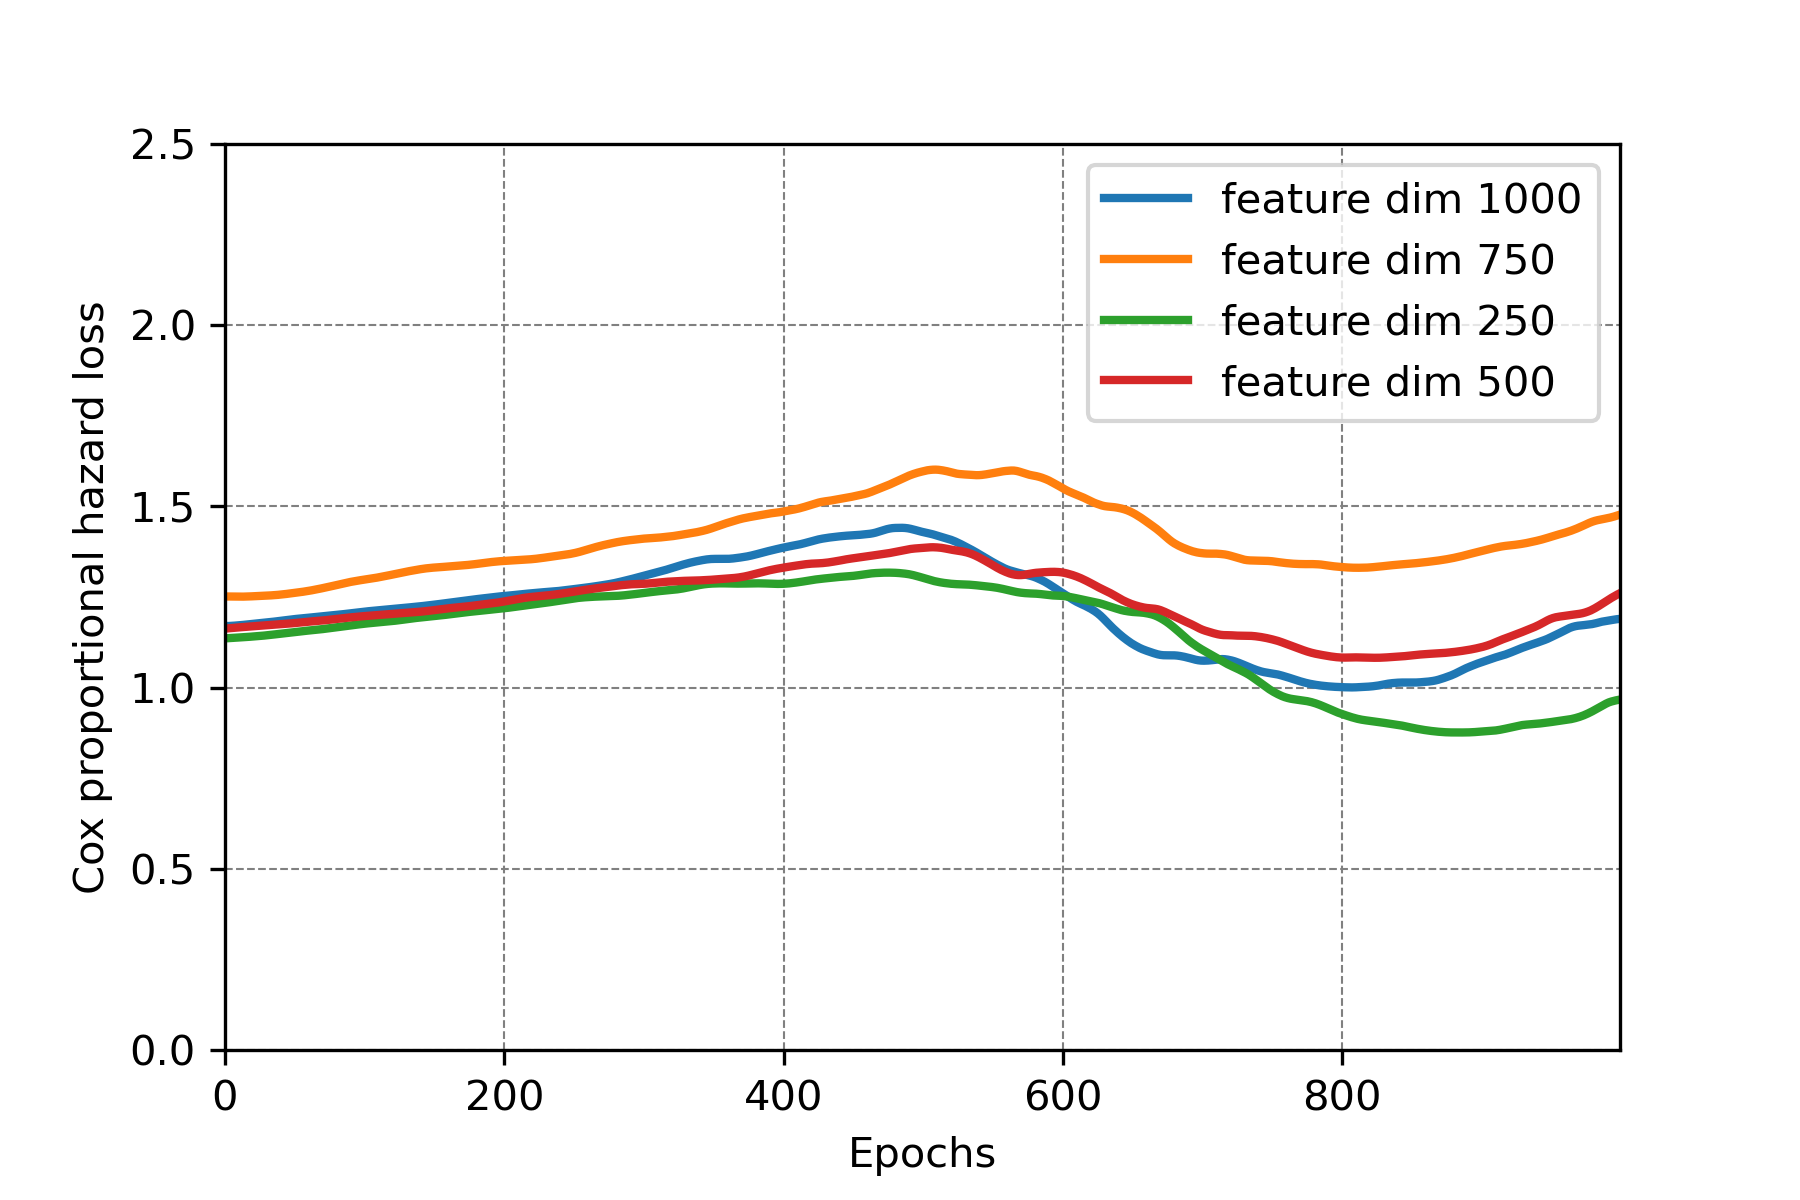
\includegraphics[width=\textwidth]{latex/loss_plots/snn_fsz_val.png}
         \caption{Validation loss}
     \end{subfigure}
    \hfill
     \begin{subfigure}[b]{0.49\textwidth}
         \centering
         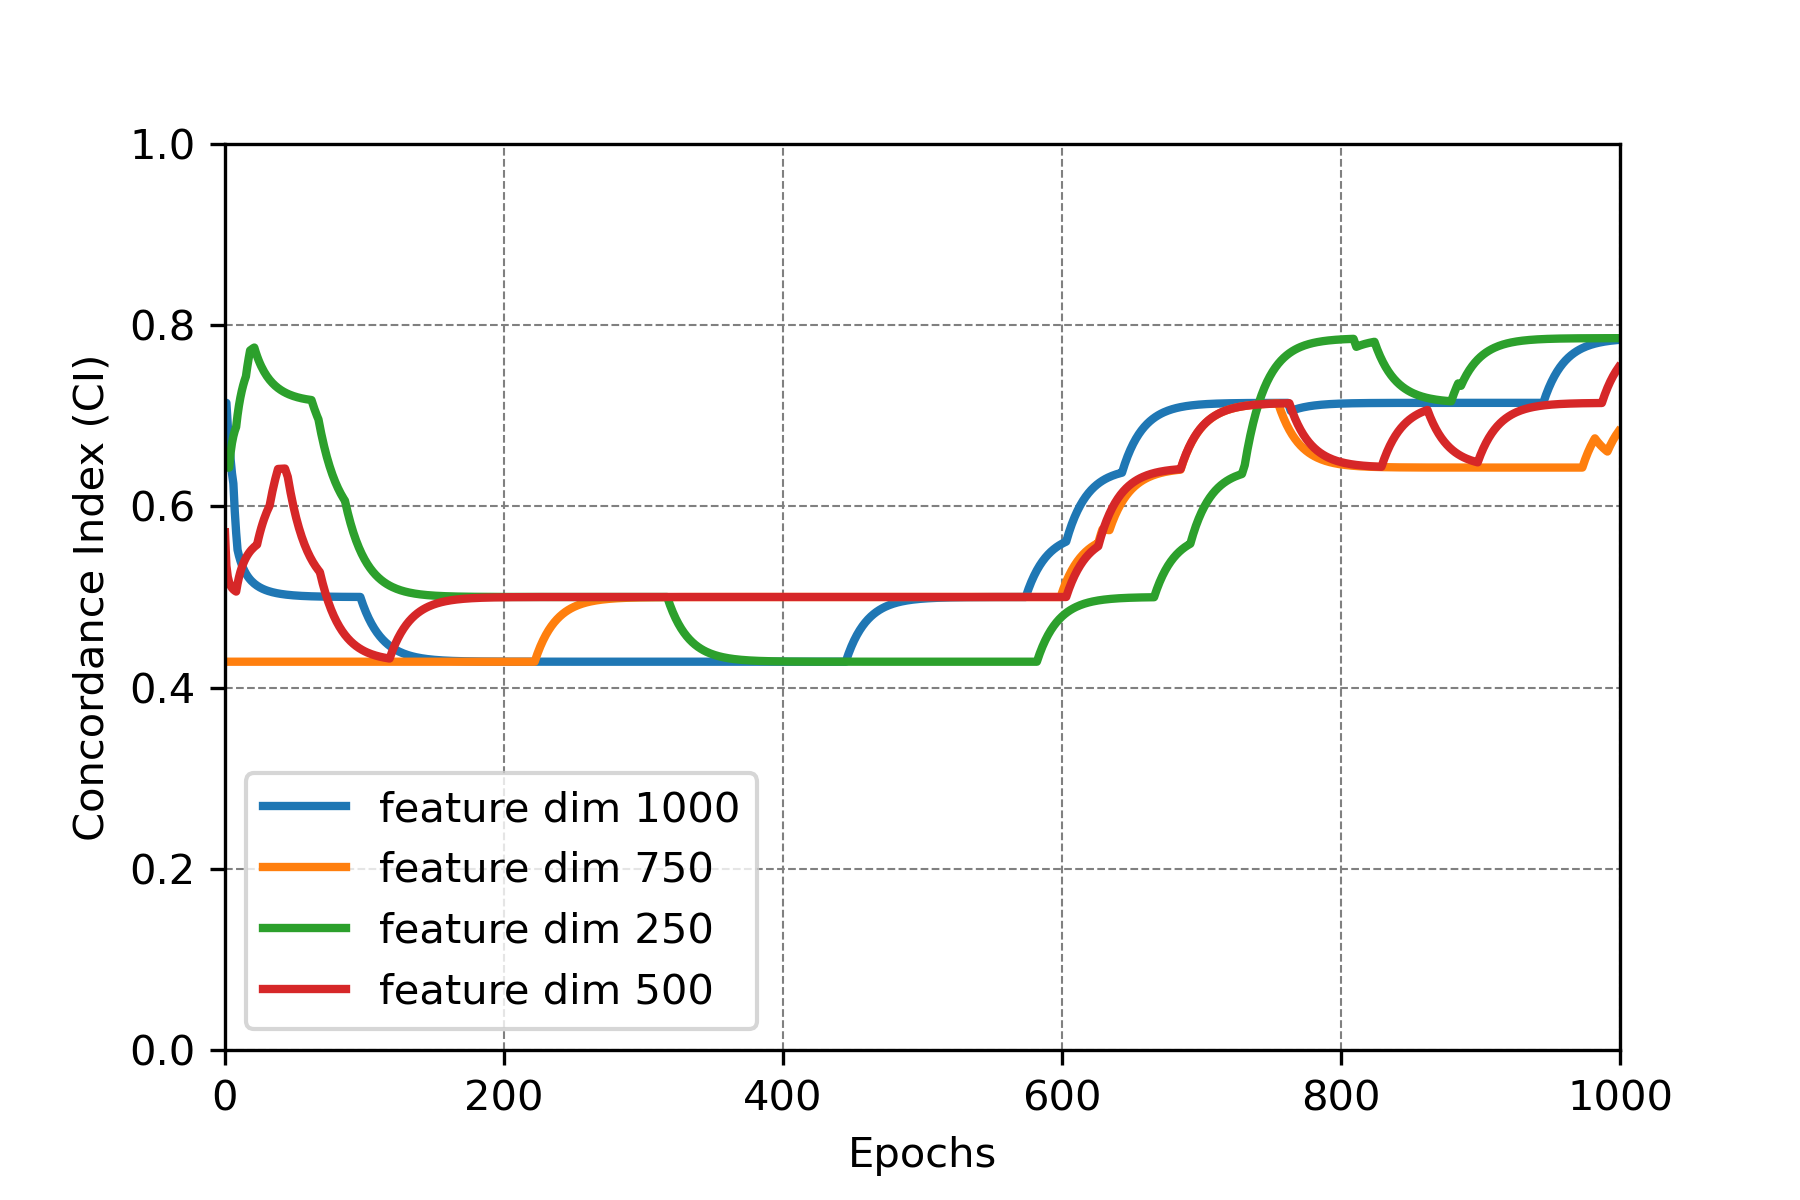
\includegraphics[width=\textwidth]{latex/ci_plots/snn_fsz_val_ci.png}
         \caption{Validation concordance index}
     \end{subfigure}
    \hfill
    \caption[Experiments on feature size for SNN]{Experiments on feature size for SNN. All parameters of the network stayed the same, except for the output size parameter of the second last fully connected layer of the network. All models were trained for the same duration on the same hardware. Each curve was smoothed using exponential moving averages with a window of 30 samples.}
    \label{fig:snn_fsz}
\end{figure}

As mentioned above, the SNN was trained at different learning rates, for which the results can be seen in figure \ref{fig:snn_lr_loss}. Additionally, the model was also evaluated with the amount of hidden layers reduced to one. 
We observe that, if only using one hidden layer, the local minimum is reached much earlier than in the experiments in \ref{fig:snn_fsz}. However, it rises in the same manner while the training loss is steadily decreasing. Altering the learning rate by one decimal position impacts the loss dramatically. We notice that the maximum validation loss reached is higher the lower the learning rate is. Furthermore, the rise is also much steeper. In all cases, the validation loss eventually increases while the training loss decreases. What differentiates the experiments is the time point when this starts occurring and the speed at which it happens.
These experiments were run for 2500 epochs to better understand the long term development of the loss. The corresponding CI curves can be found in the appendix in figure \ref{fig:snn_lr_ci}

\begin{figure}[h!t]
    \centering
 \begin{subfigure}[b]{0.49\textwidth}
     \centering
     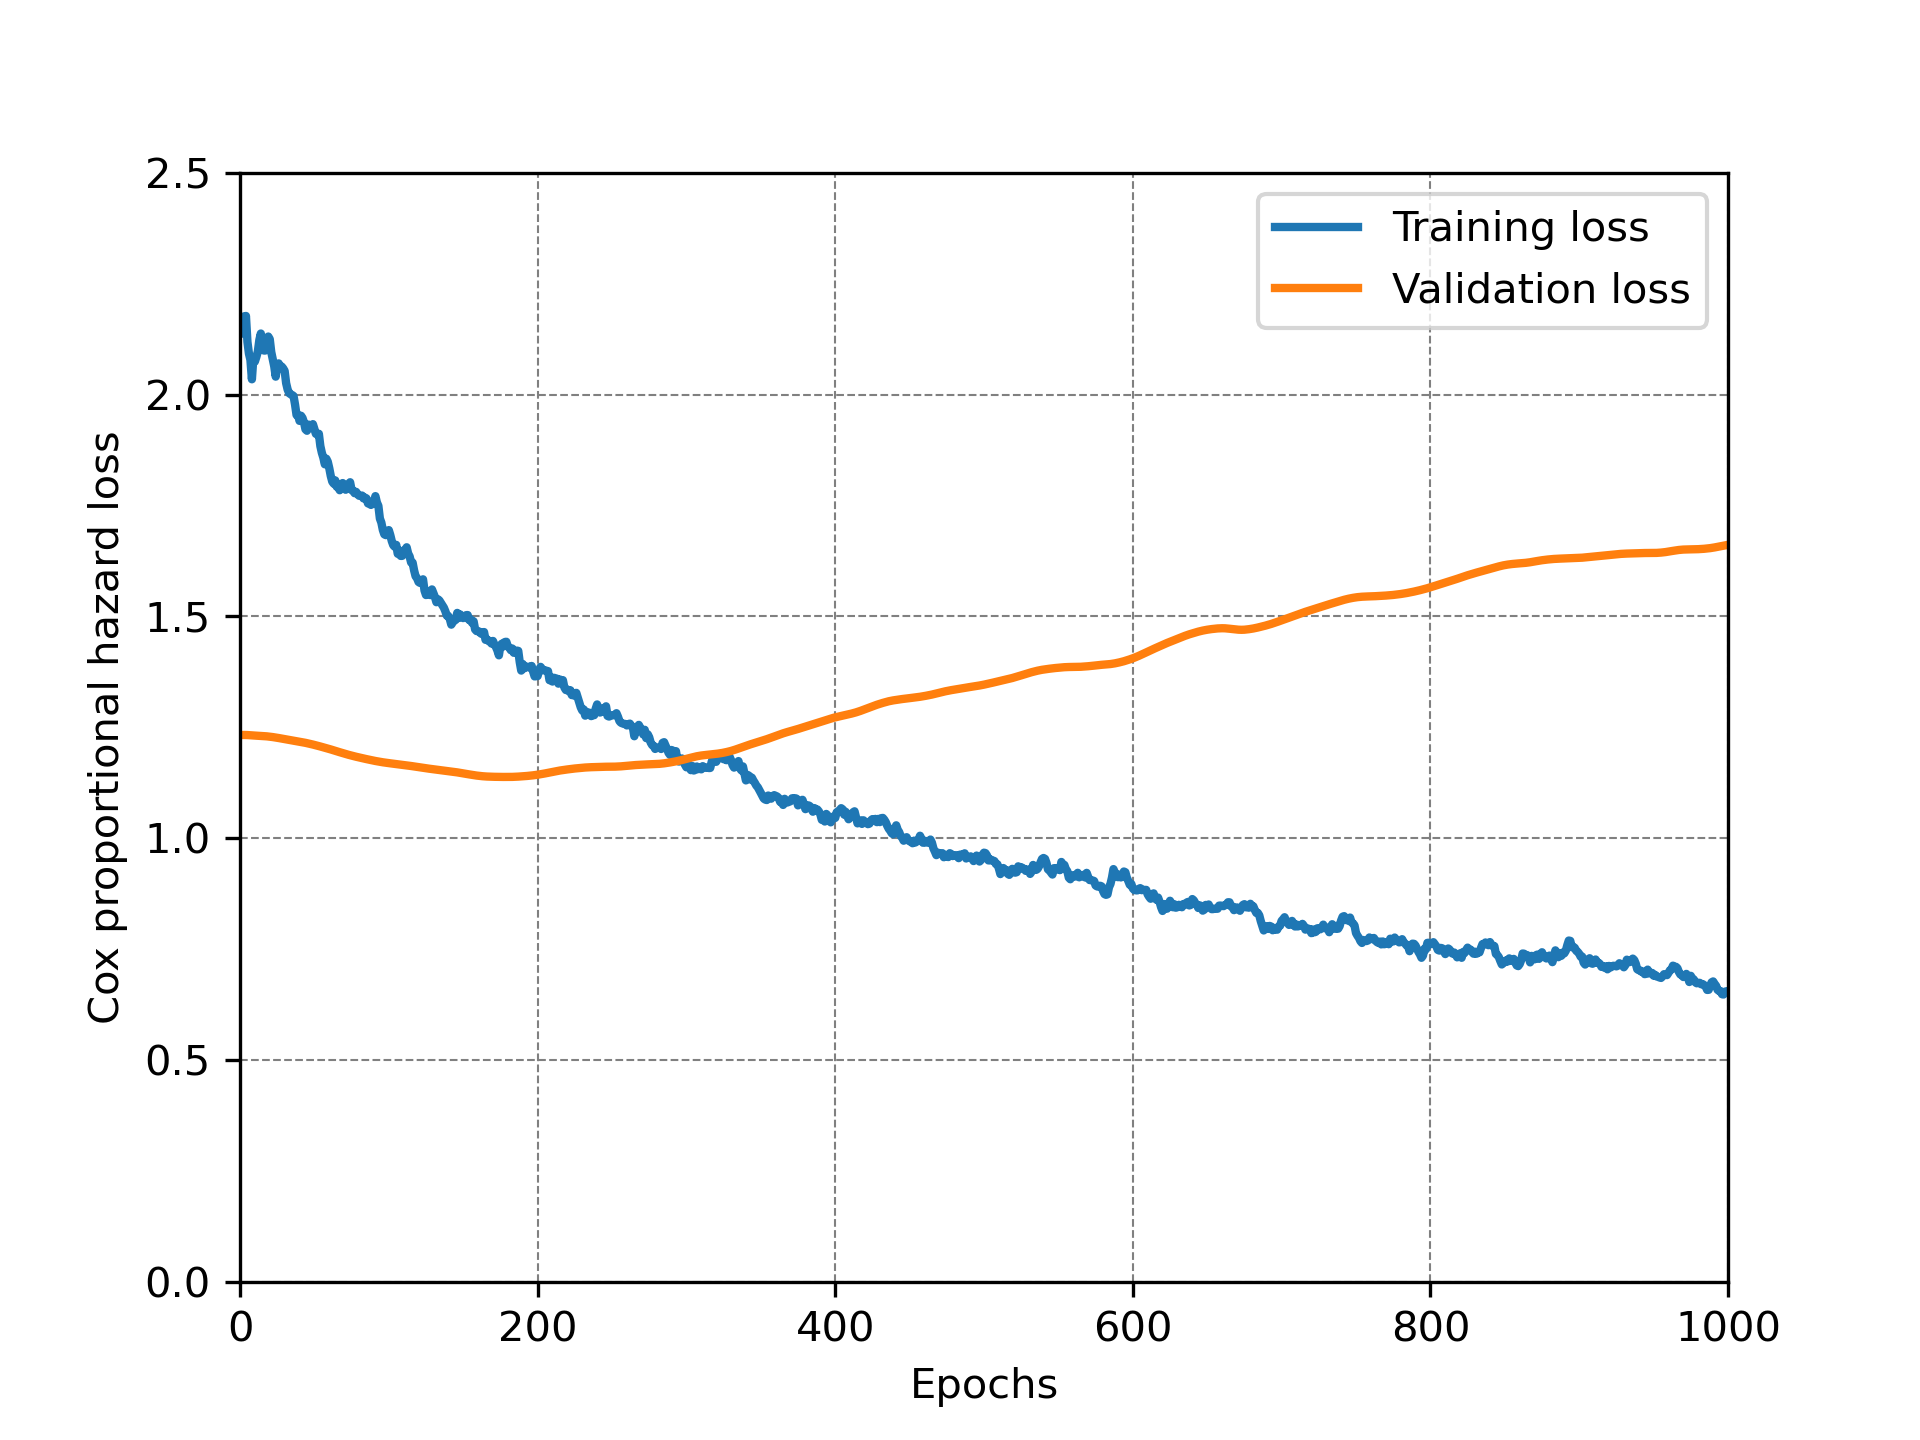
\includegraphics[width=\textwidth]{latex/loss_plots/SNNet_fsz250_1Layer.png}
     \caption{SNN with single hidden layer}
 \end{subfigure}
    \hfill
     \begin{subfigure}[b]{0.49\textwidth}
         \centering
         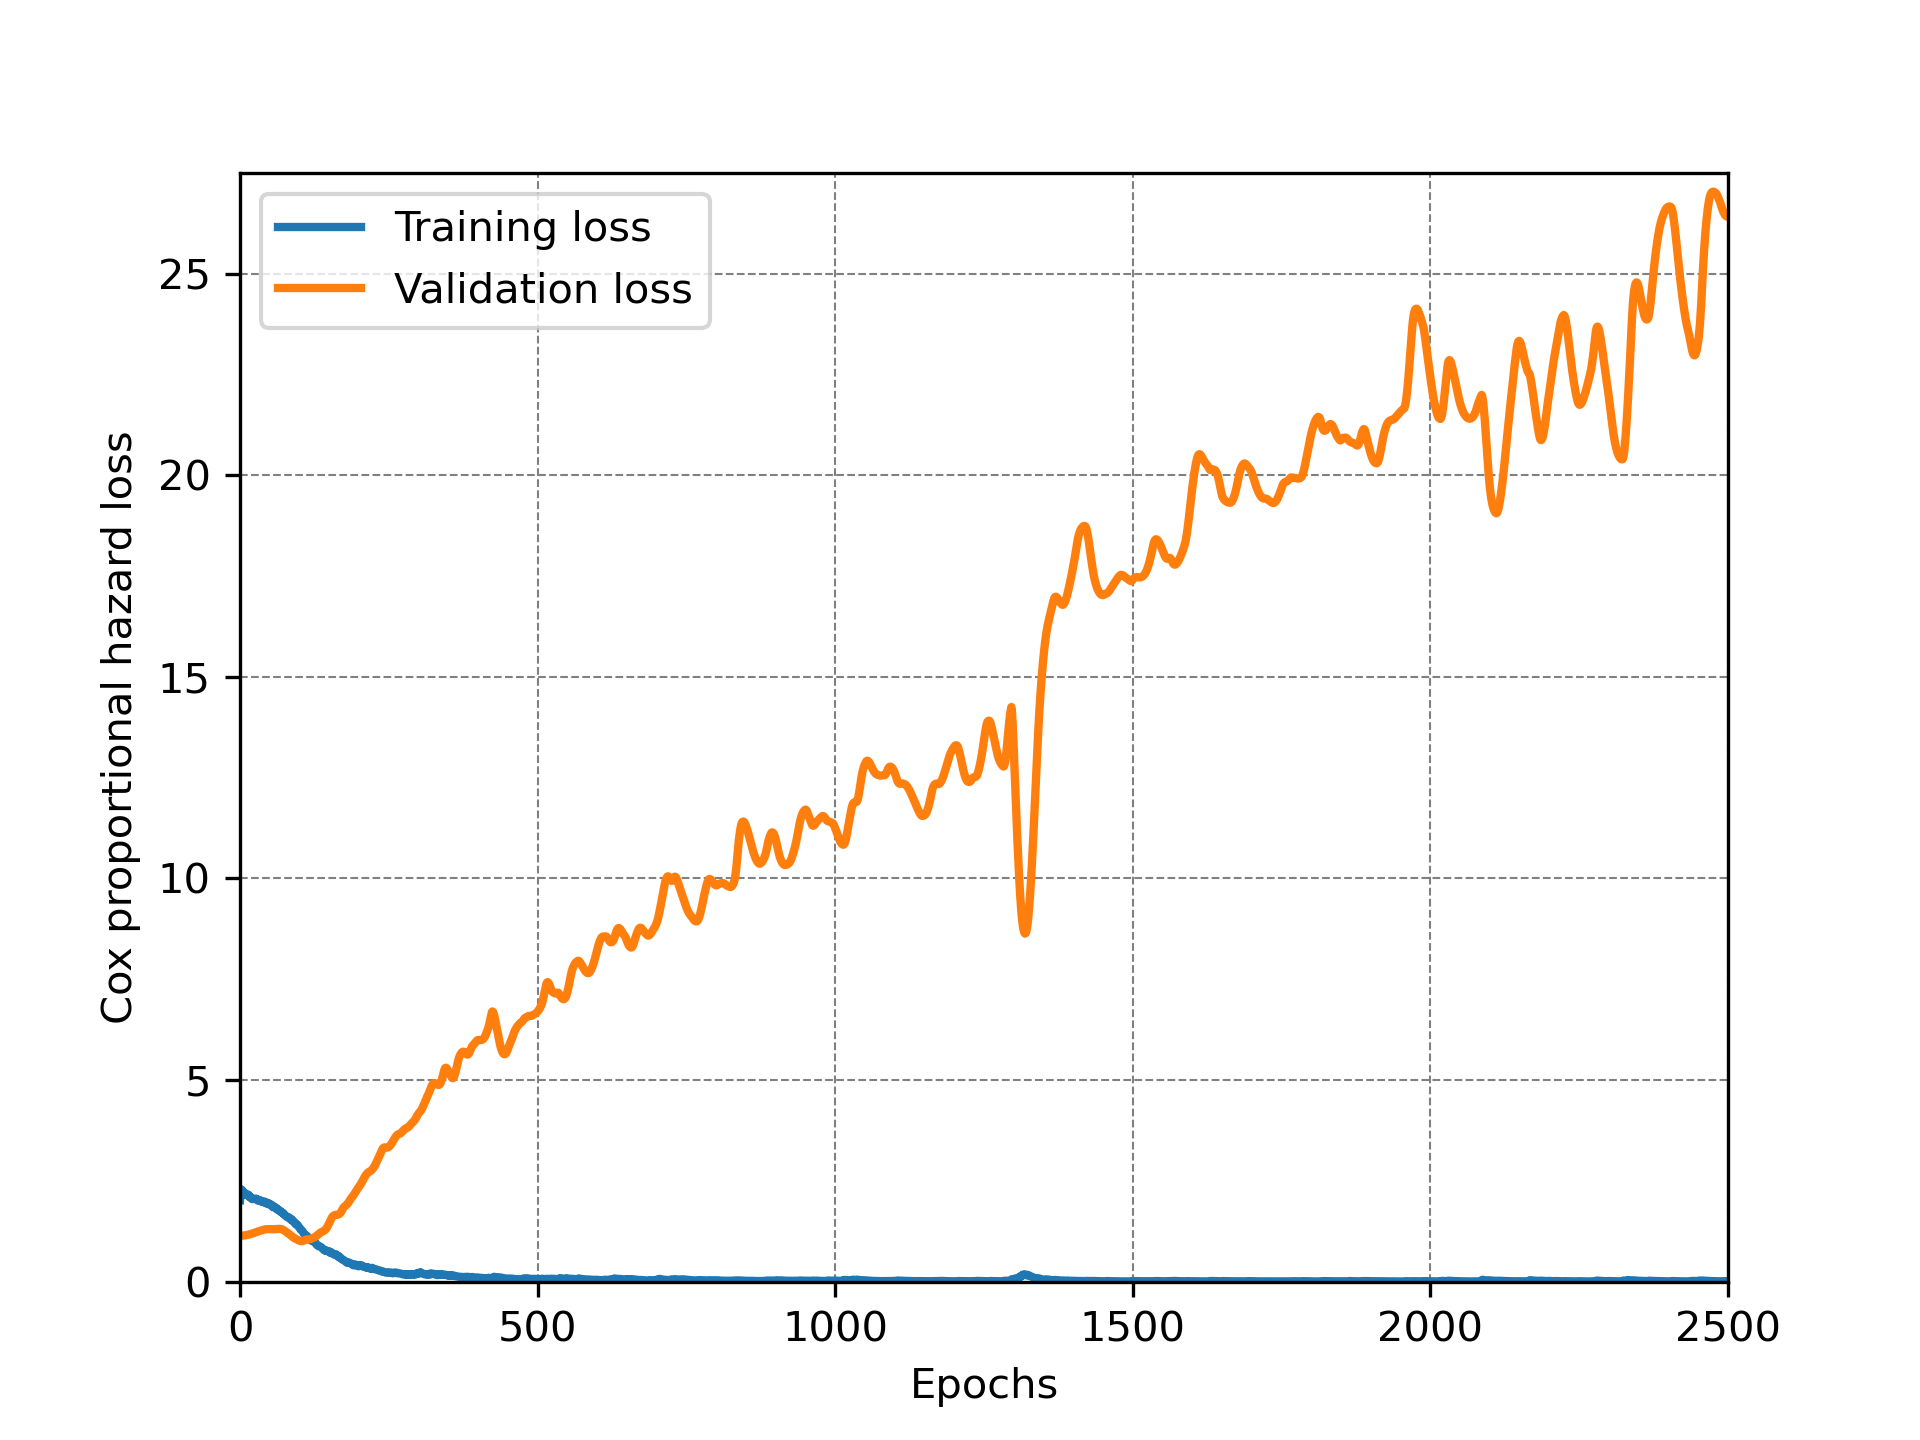
\includegraphics[width=\textwidth]{latex/loss_plots/SNNet_fsz250_1e-4_2500epochs.png}
         \caption{SNN at lr 1e-4}
     \end{subfigure}
\vskip\baselineskip
     \begin{subfigure}[b]{0.49\textwidth}
         \centering
         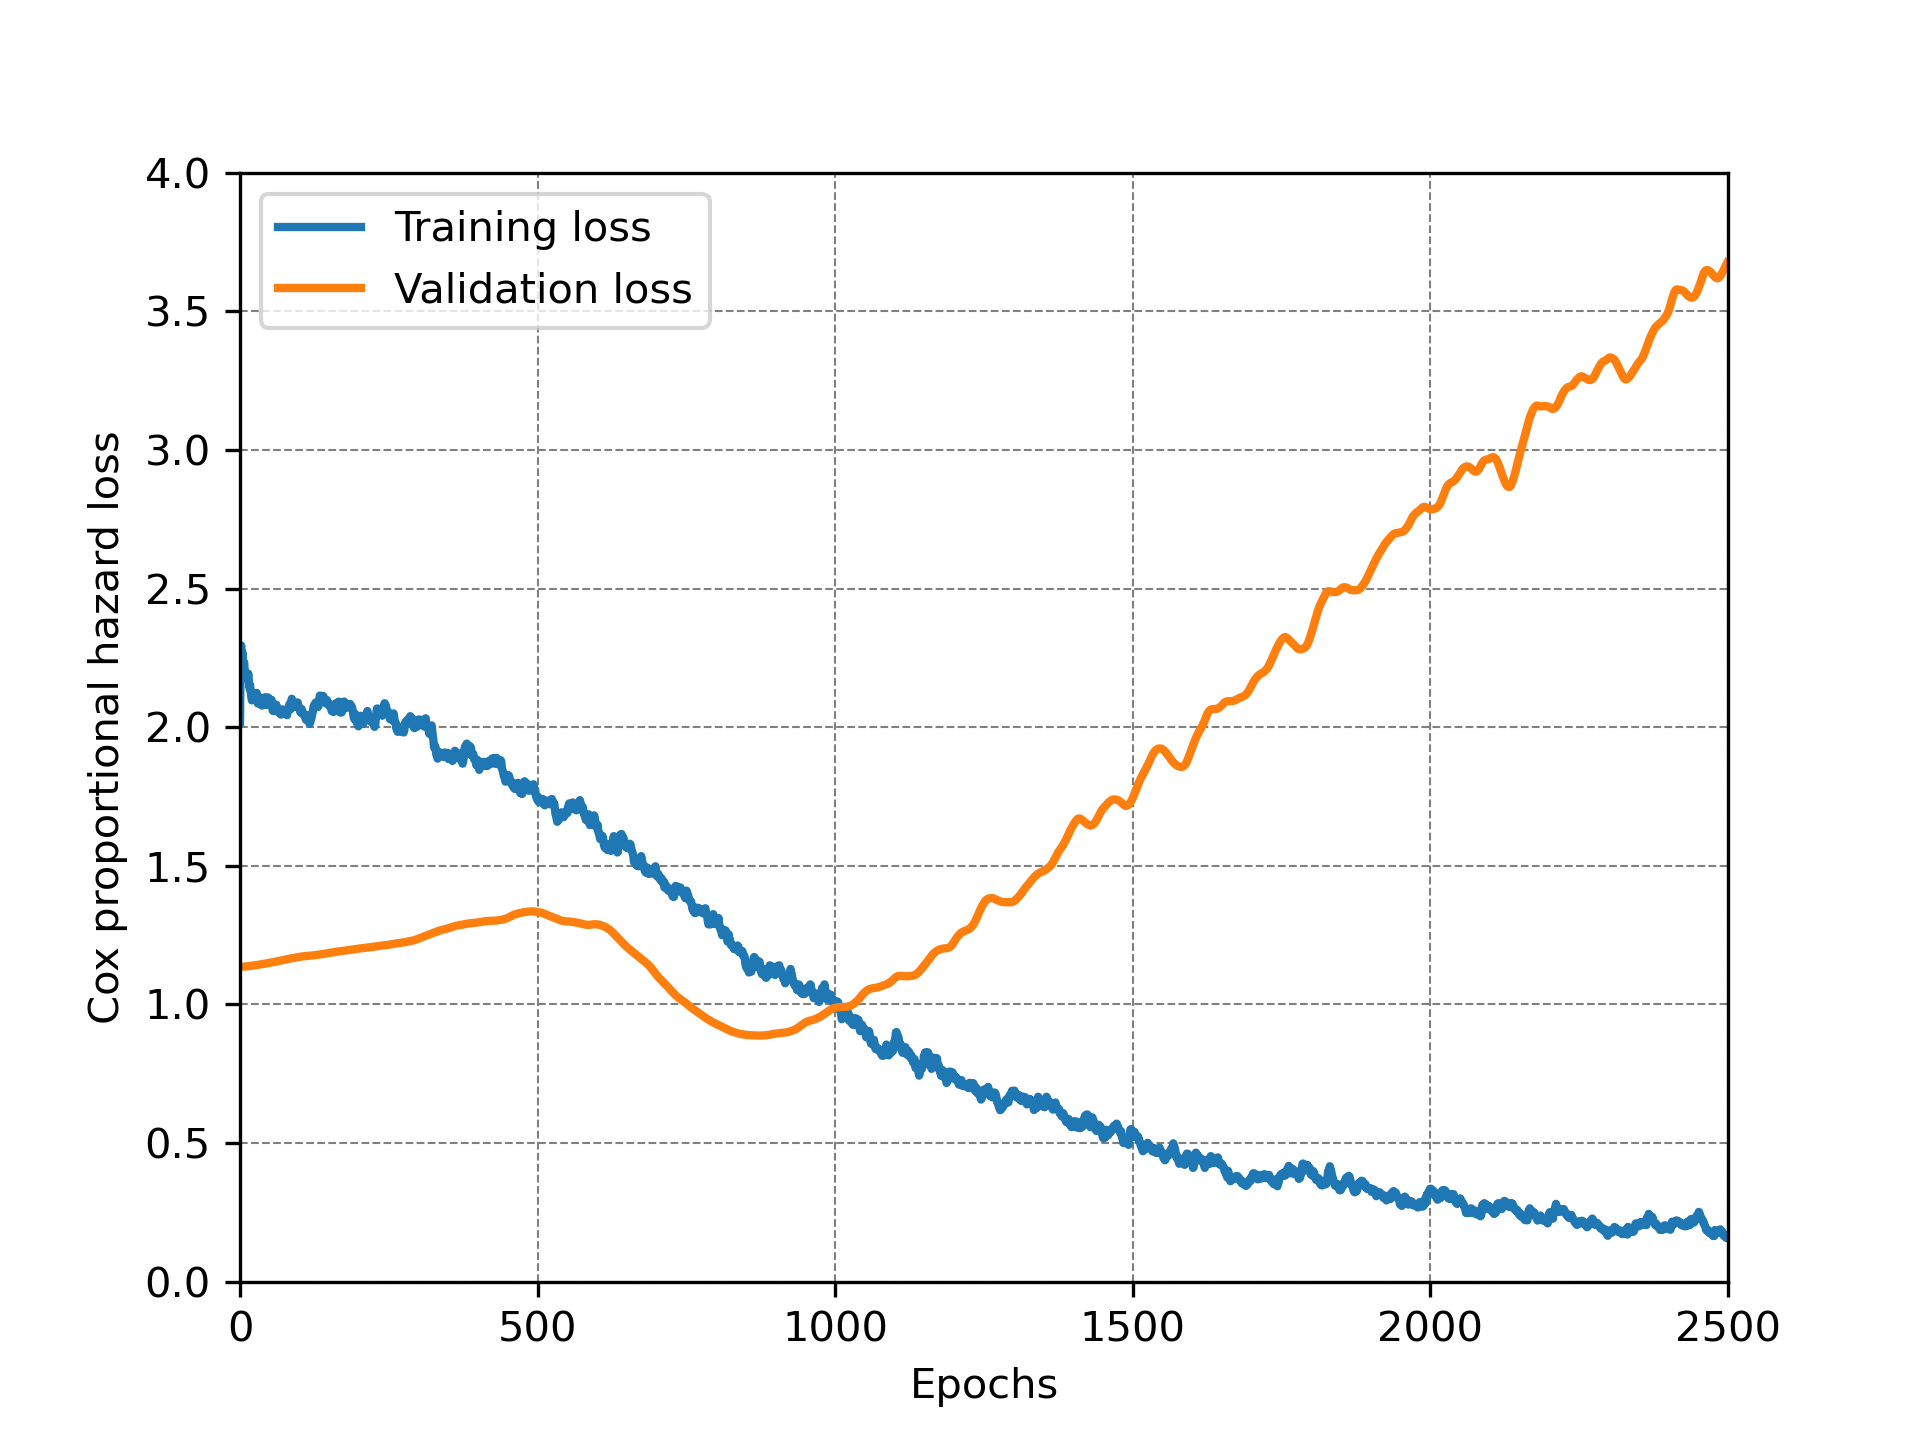
\includegraphics[width=\textwidth]{latex/loss_plots/SNNet_fsz250_1e-5_2500epochs.png}
         \caption{SNN at lr 1e-5}
     \end{subfigure}
    \hfill
     \begin{subfigure}[b]{0.49\textwidth}
         \centering
         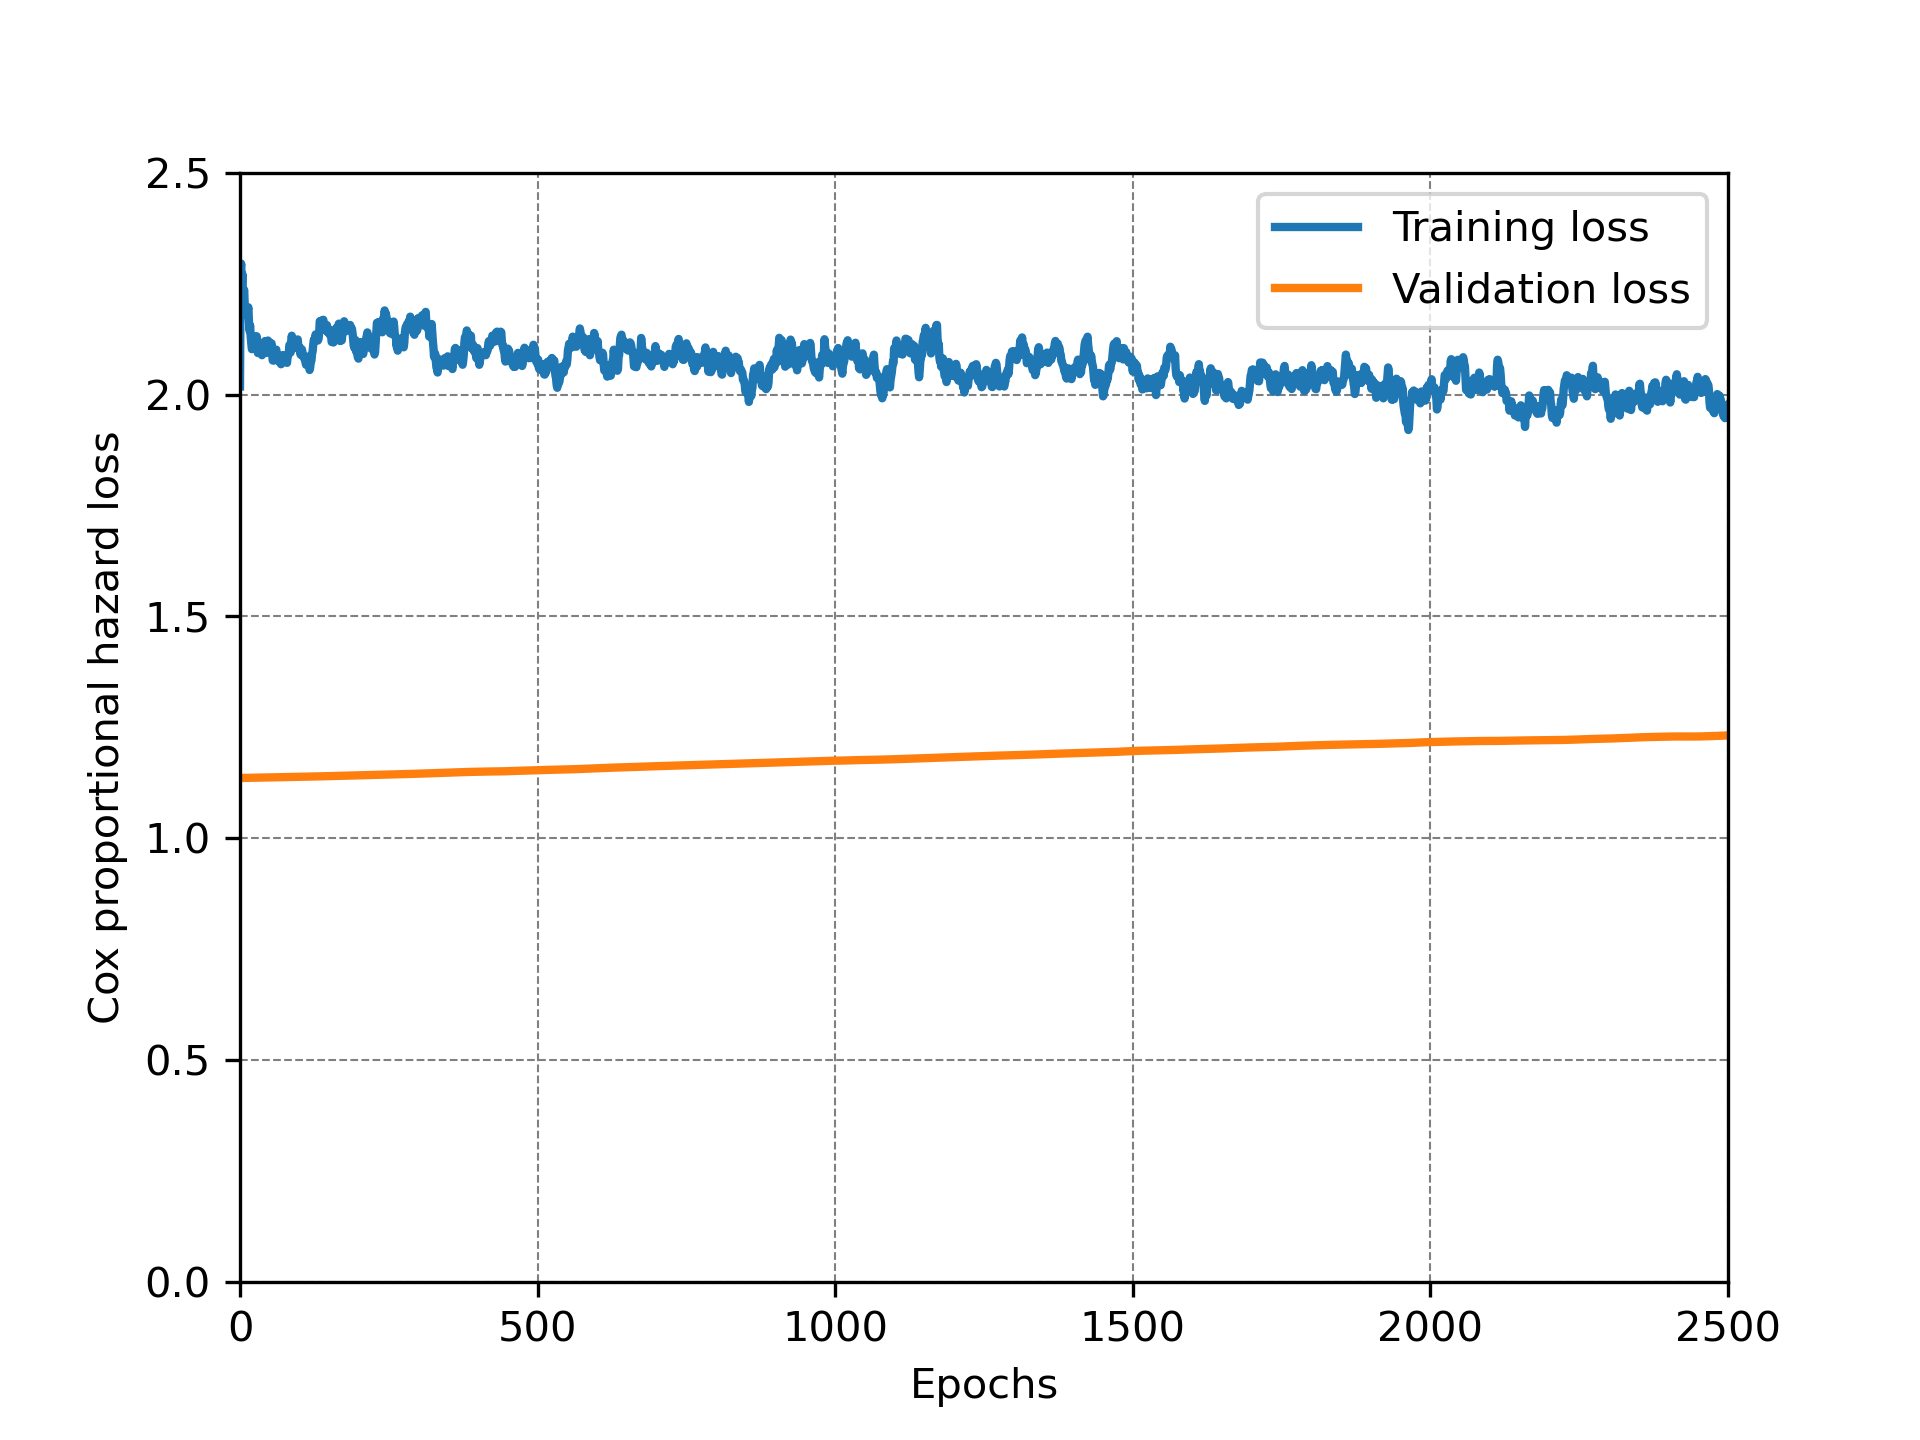
\includegraphics[width=\textwidth]{latex/loss_plots/SNNet_fsz250_1e-6_2500epochs.png}
         \caption{SNN at lr 1e-6}
     \end{subfigure}
    \hfill
    \caption[SNN with varying learning rates and models]{Experiments for SNN on learning rates and number of hidden dimensions. Neither x-axis nor y-axis are uniform.}
    \label{fig:snn_lr_loss}
\end{figure}

The final model that was decided upon, uses a dropout rate of 0.25, a learning rate of 1e-5 and its last hidden layer produces a vector of size 1000. This model is used in the following section for building the fusion models.

\clearpage

\section{Fusion comparison}

Due to concerns regarding the required time, each fusion experiment was run for only 300 epochs. We assume that this should be enough to determine the most promising fusion technique, which can then be used for further optimisations. Each experiment still required at least 9 hours of time to complete.
Figures \ref{fig:fusions_simple} and \ref{fig:fusions_complex} shows the result of the six different approaches that have been tested. Except of the particular fusion mechanic, all parameters were the same. From table \ref{tab:c_indices_fuse} and the figures, we can observe that the approaches there are indeed notable differences. Especially, the Kronecker approach seems to stagnate over the course of training. 
The training losses are higher on average since their calculation is cumulative and the size of the respective dataset is larger. Hence, comparisons of different losses within a dataset are more appropriate than between the datasets. 
It should also be noted that the metrics in Table \ref{tab:c_indices_fuse} correspond to the latest model, after the last epoch, rather than the best performing one. As the presented results only serve as an indication of the particular learning progress of the model, it is more reasonable to compare them at the same time point. Each model would be needed to be trained to convergence first before an evaluation of the best possible performance is reasonable. 

\begin{table}[h!b]
    \centering
    \caption[Fusion networks metrics]{Concordance Indices and negative log likelihoods of different fusion approaches. Losses to the left, and concordance indices to the right.}
    \begin{tabular}{l | c c c | c c c }
         \hline
        \multirow{2}{*}{} & \multicolumn{3}{c|}{Concordance index} & \multicolumn{3}{c}{Likelihood Loss} \\ [0.5ex]
        \hline
       Experiment & Training & Validation & Test & Training & Validation & Test \\ [0.5ex]
       \hline  
        Maximum        & 0.594 & 0.590 & 0.618  & 2.025 & 0.648 & 0.532 \\
        Summation      & 0.637 & 0.651 & 0.566  & 1.643 & 0.681 & 0.703 \\
        Concatenated  & 0.709 & 0.522 & 0.589  & 2.148 & 1.611 & 0.616 \\
        EmbraceNet     & 0.596 & 0.644 & 0.486  & 1.041 & 0.706 & 0.752 \\
        Attention      & 0.492 & 0.500 & 0.549  & 1.319 & 0.652 & 0.558 \\
        Kronecker      & 0.580 & 0.594 & 0.612  & 1.117 & 0.570 & 0.570 \\
        \hline
    \end{tabular}
    \label{tab:c_indices_fuse}
\end{table}


\begin{figure}[h!b]
    \centering
     \begin{subfigure}[b]{\textwidth}
         \centering
         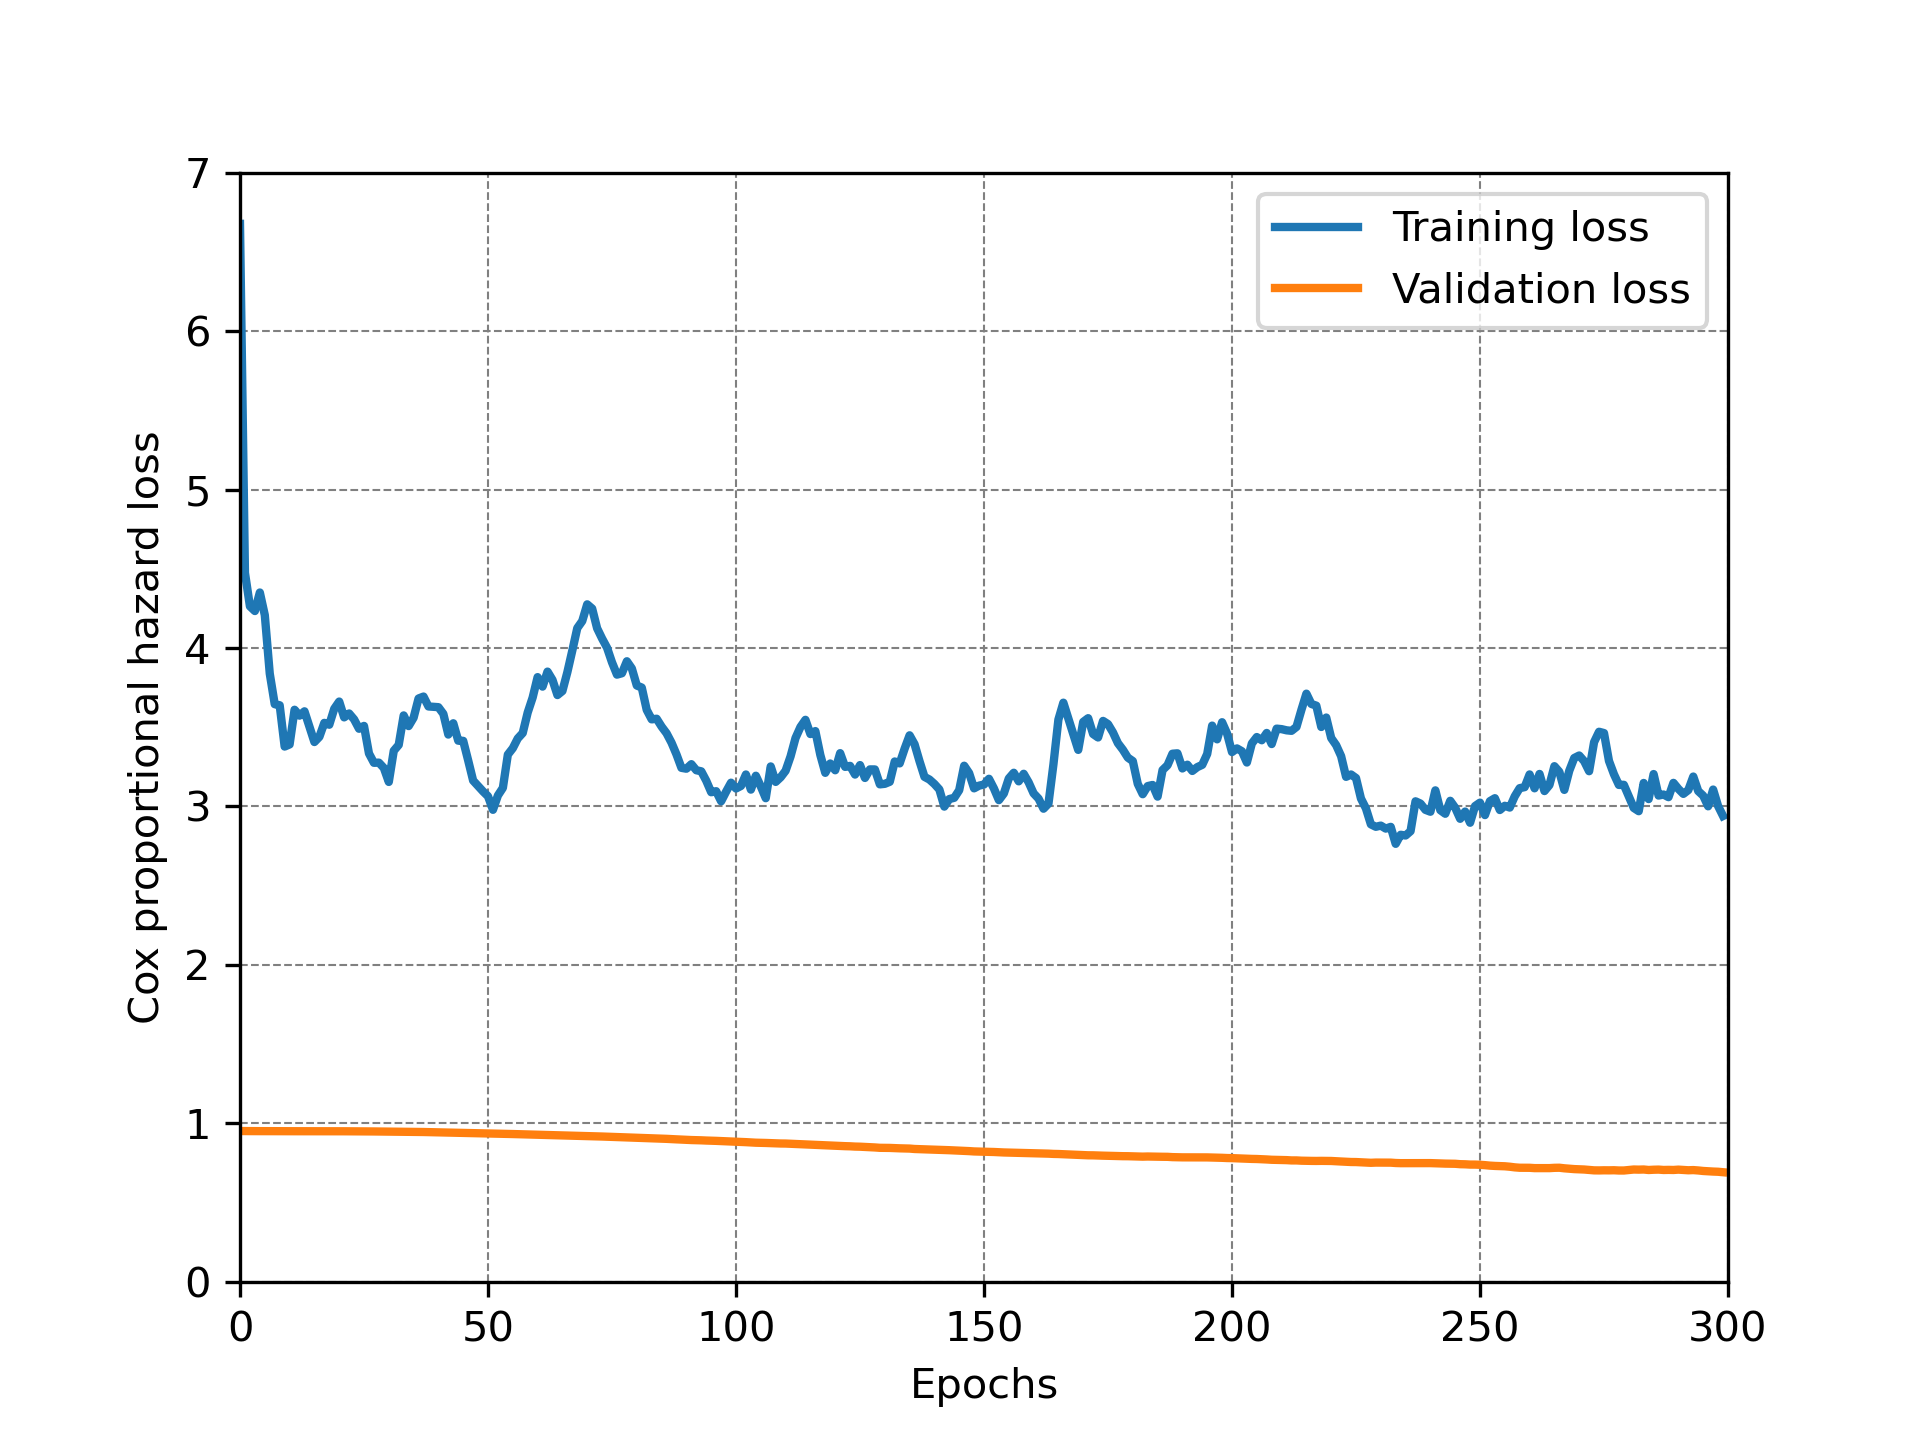
\includegraphics[width=0.49\textwidth]{latex/loss_plots/max.png}
         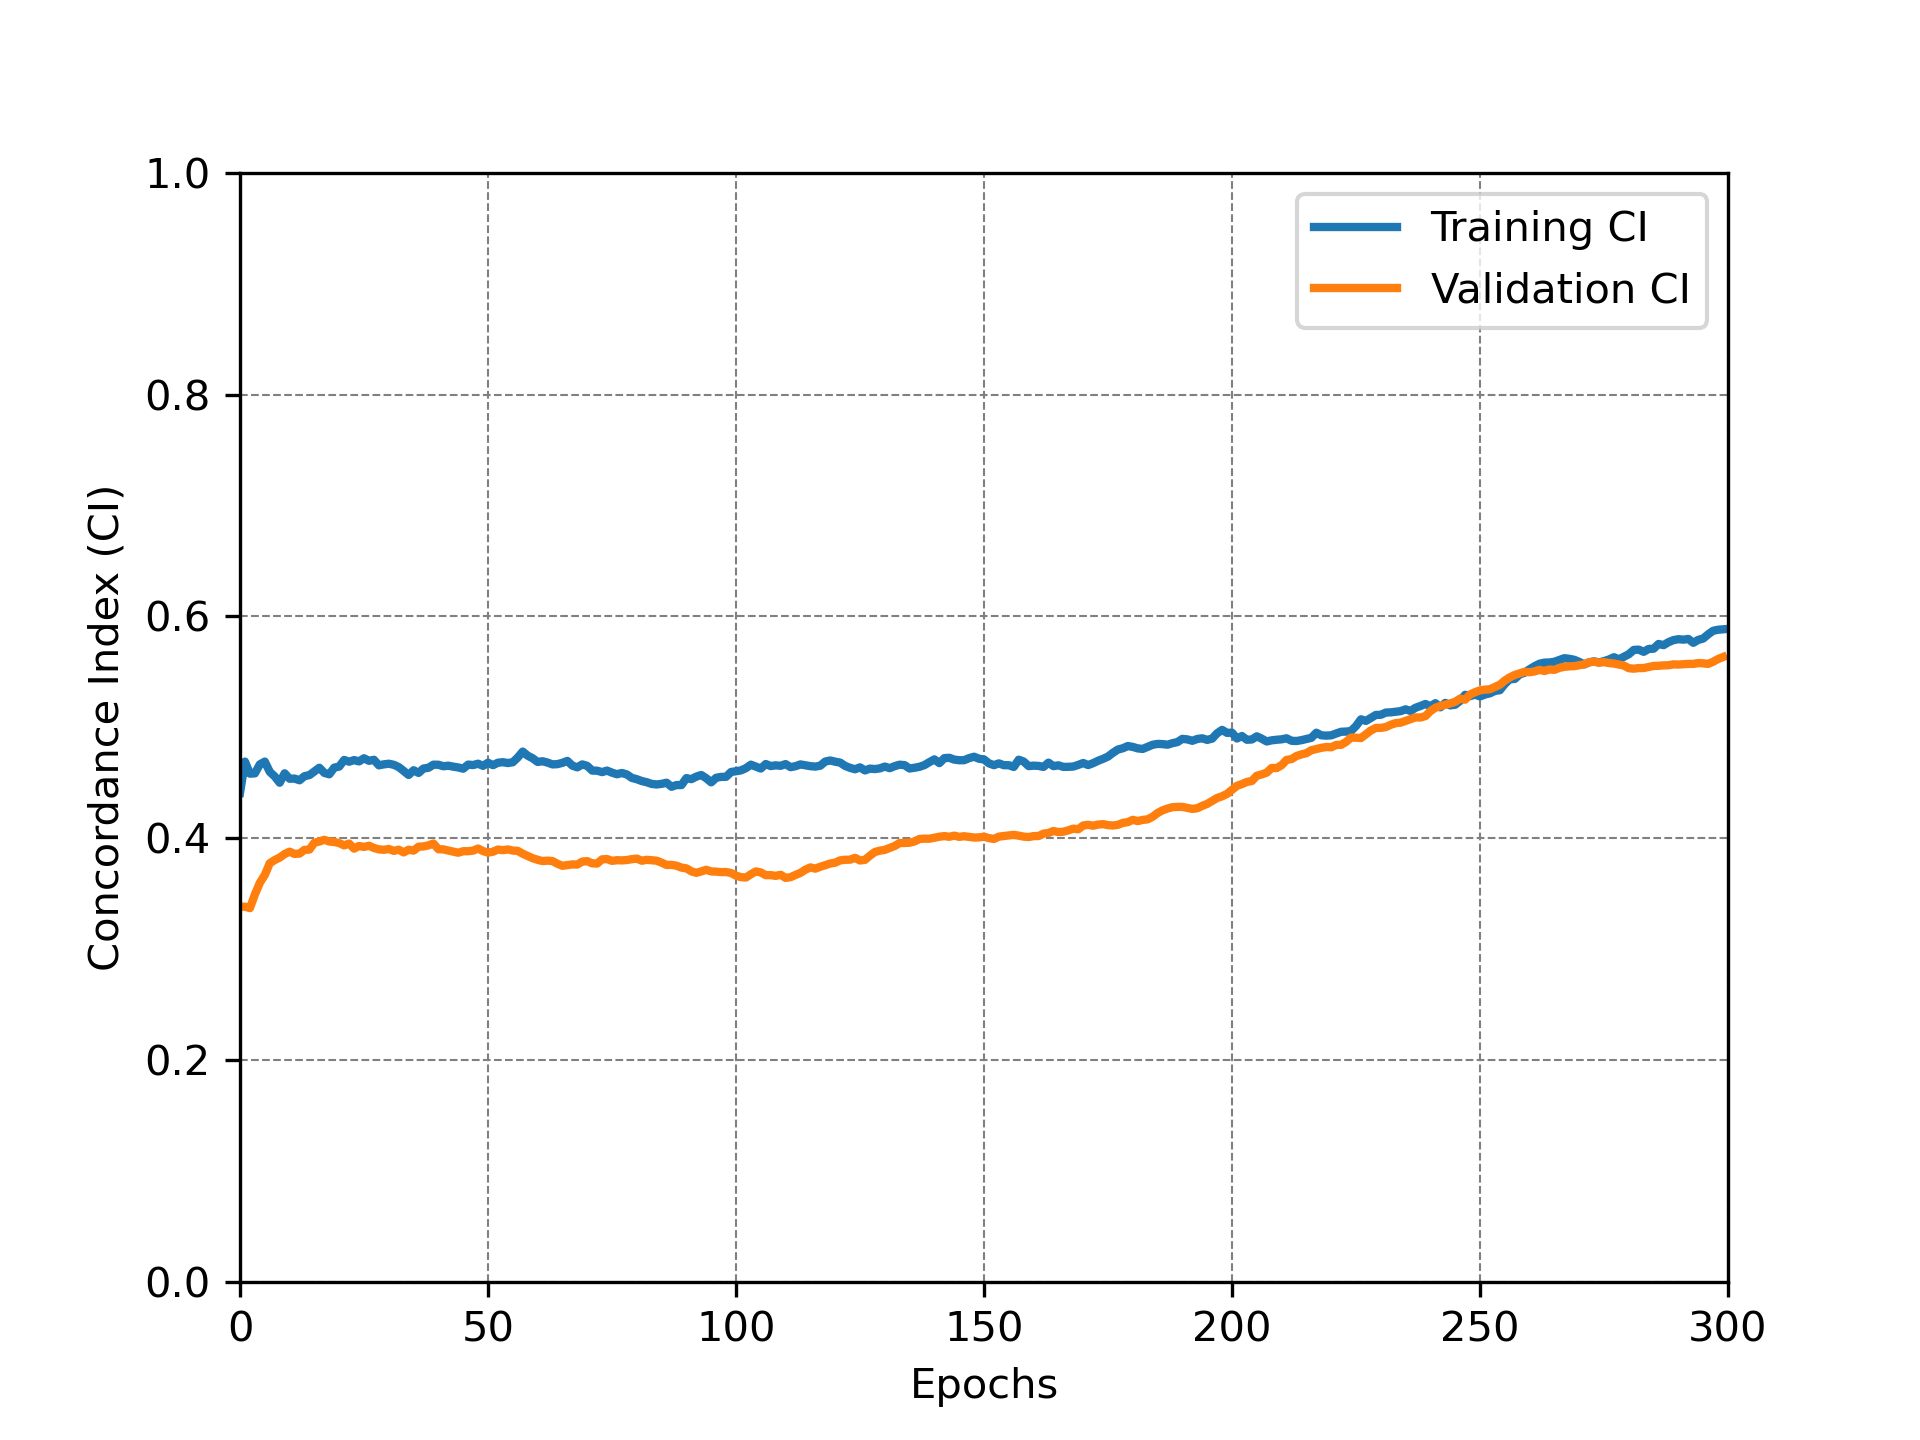
\includegraphics[width=0.49\textwidth]{latex/ci_plots/max.png}
         \caption{Element-wise maximum}
     \end{subfigure}
\vskip\baselineskip
     \begin{subfigure}[b]{\textwidth}
         \centering
         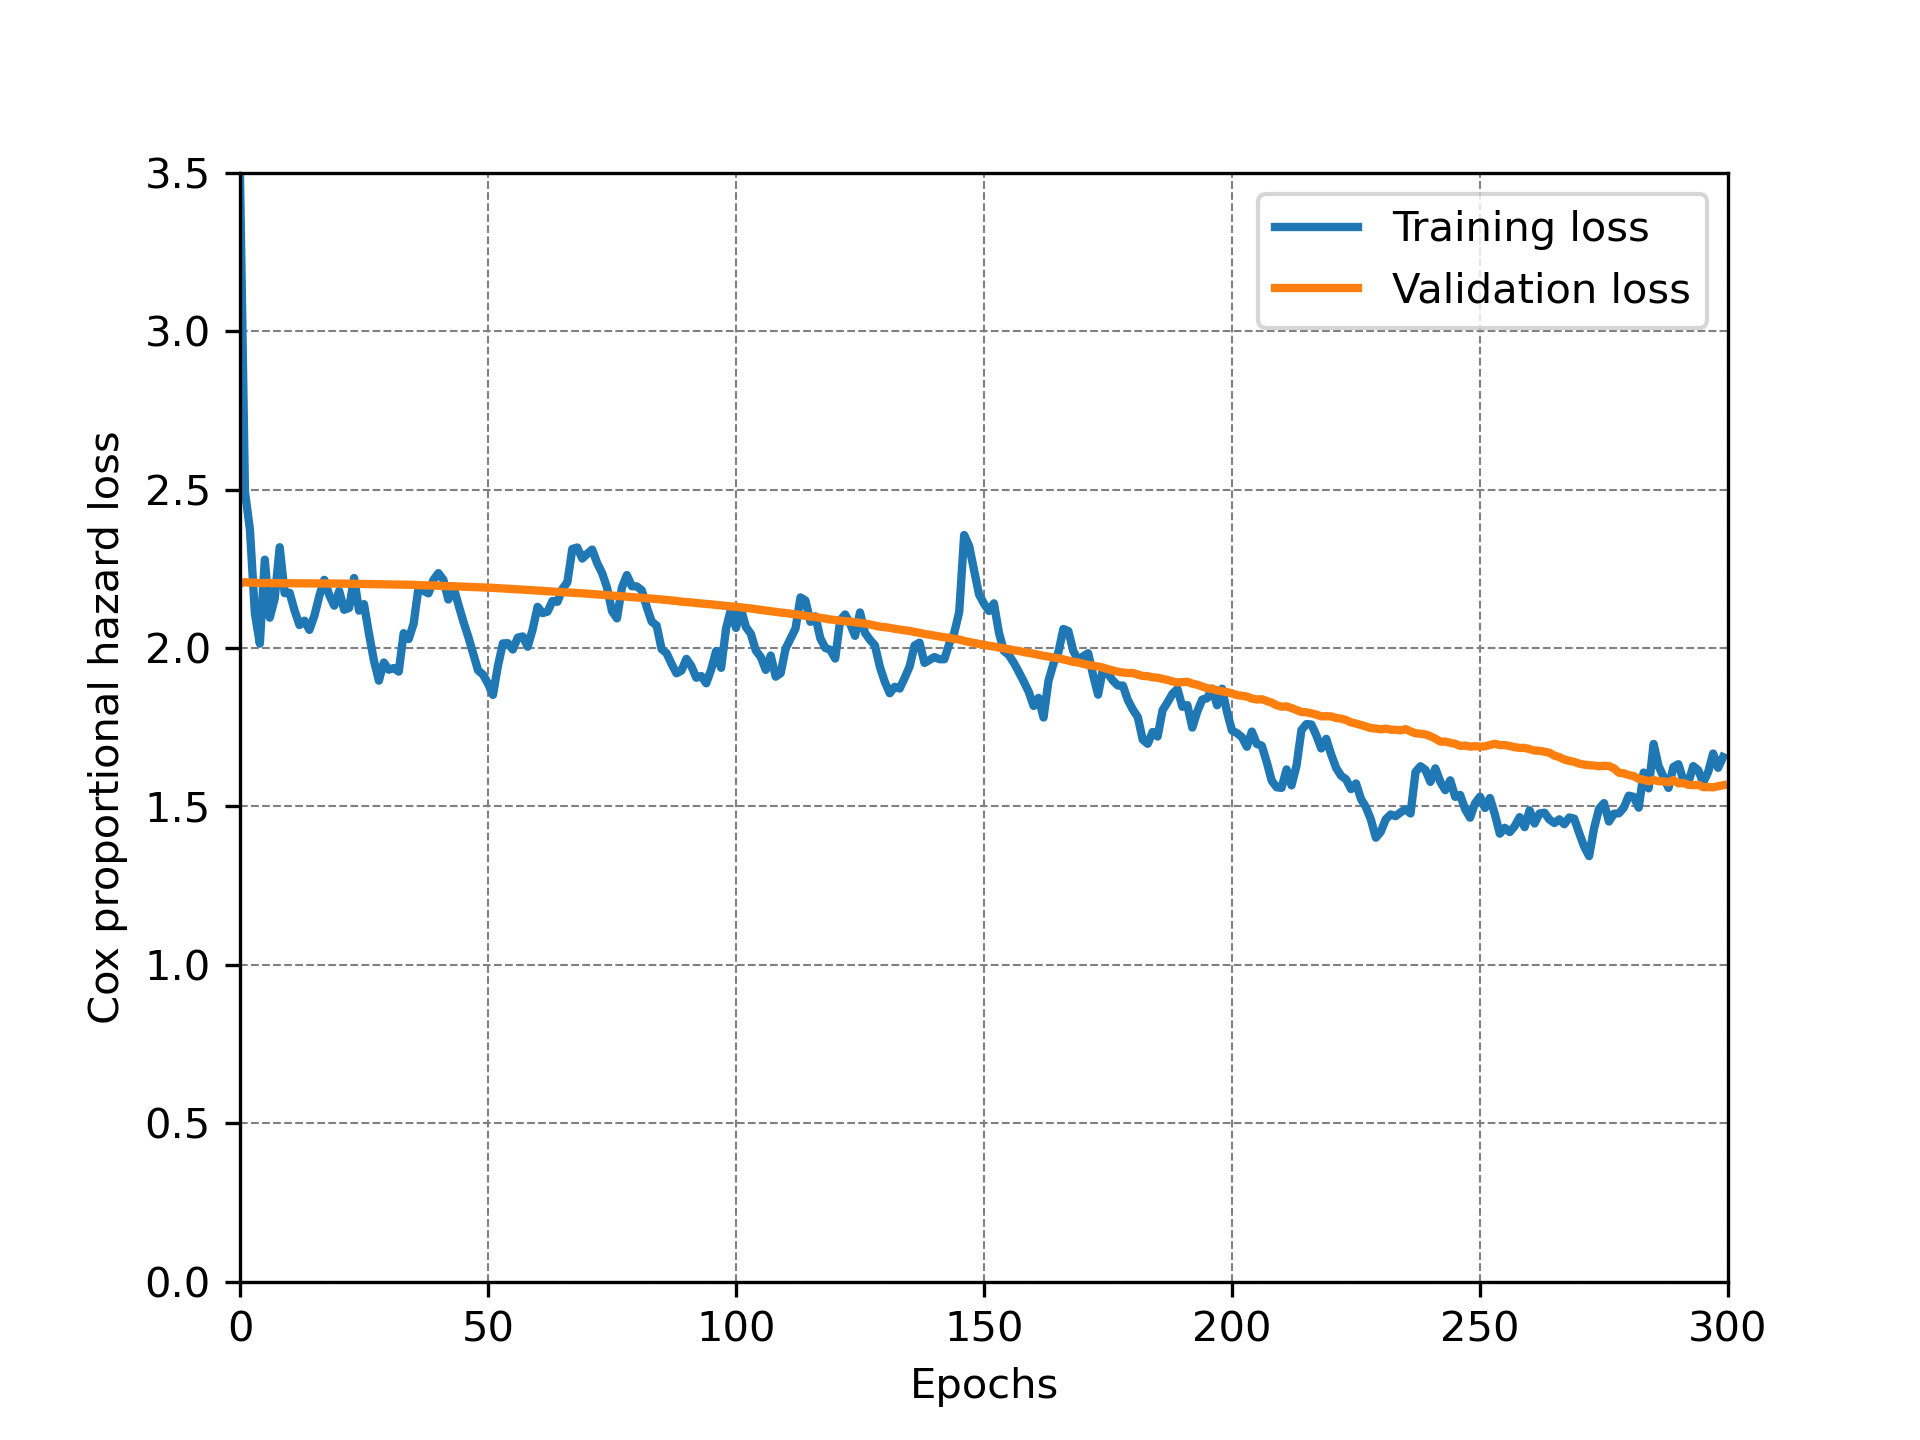
\includegraphics[width=0.49\textwidth]{latex/loss_plots/cat.png}
         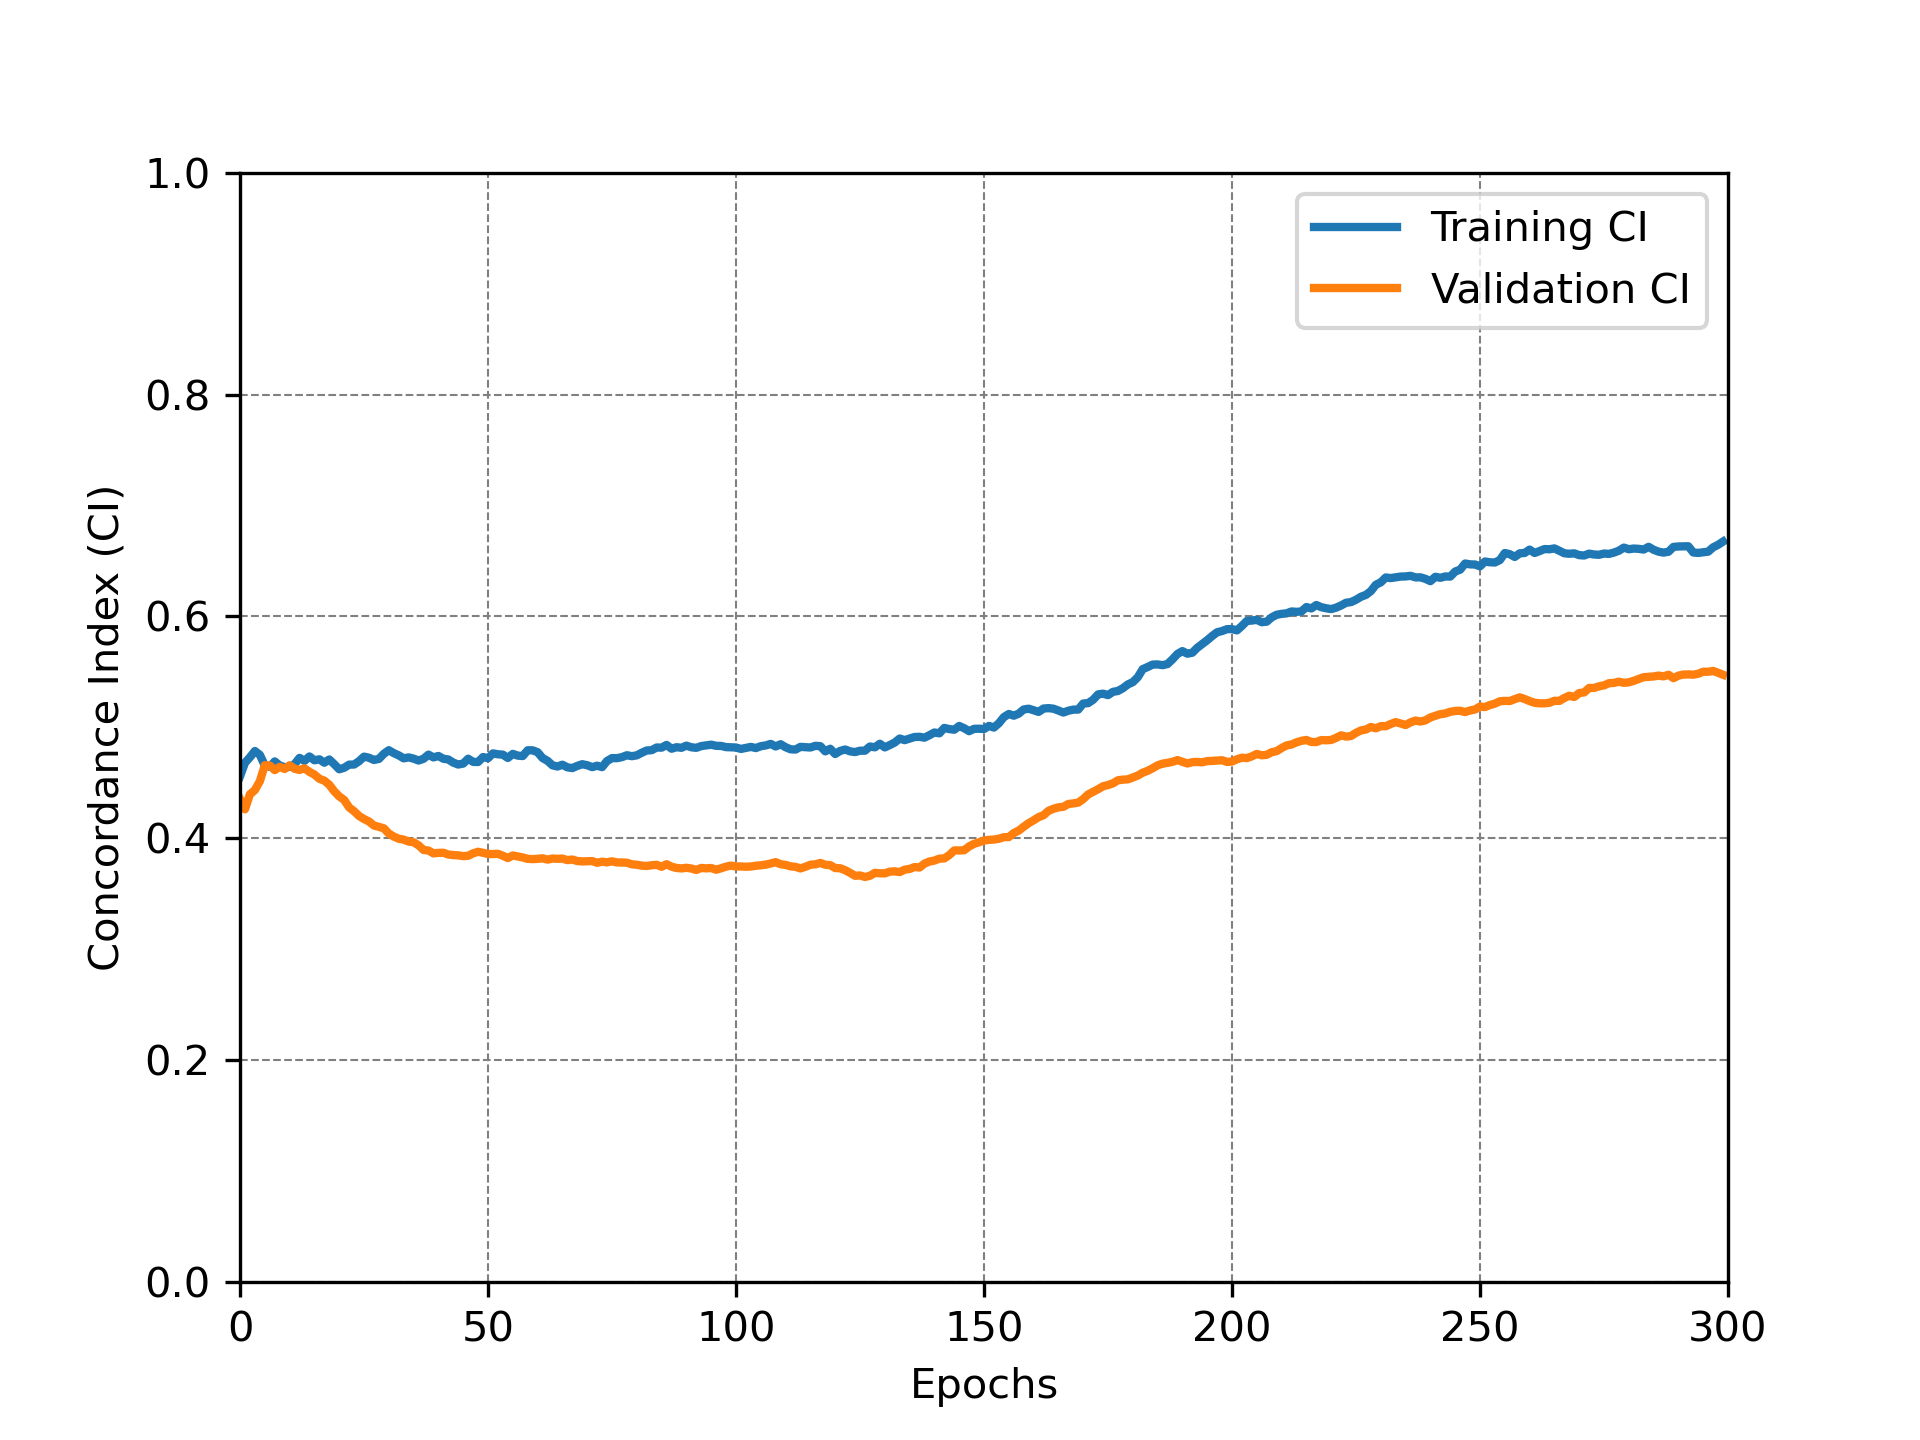
\includegraphics[width=0.49\textwidth]{latex/ci_plots/cat.png}
         \caption{Concatenation}
     \end{subfigure}
\vskip\baselineskip
     \begin{subfigure}[b]{\textwidth}
         \centering
         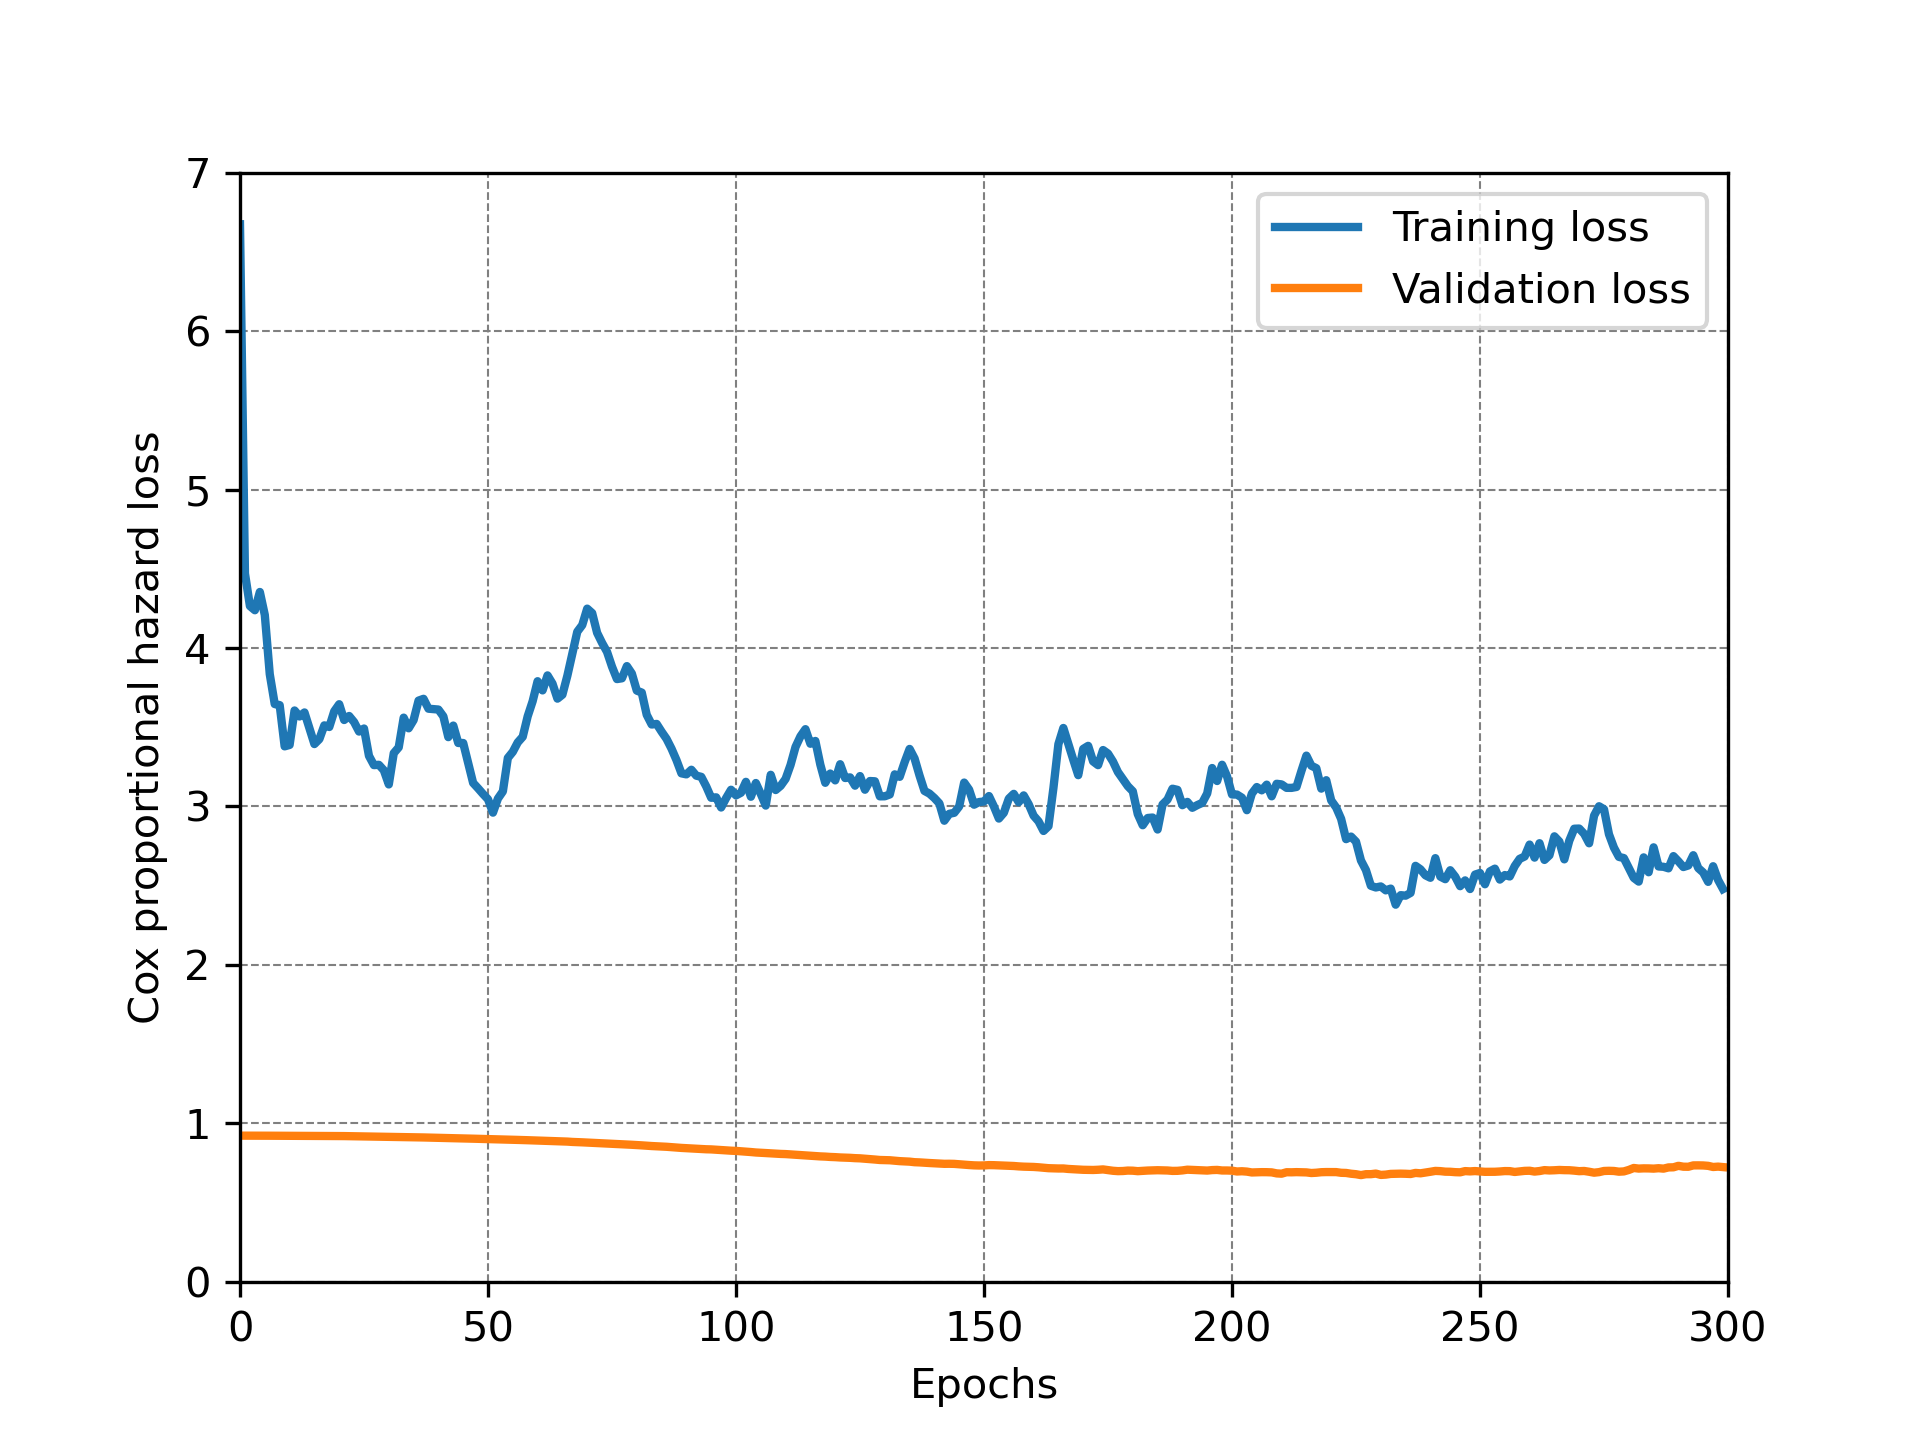
\includegraphics[width=0.49\textwidth]{latex/loss_plots/sum.png}
         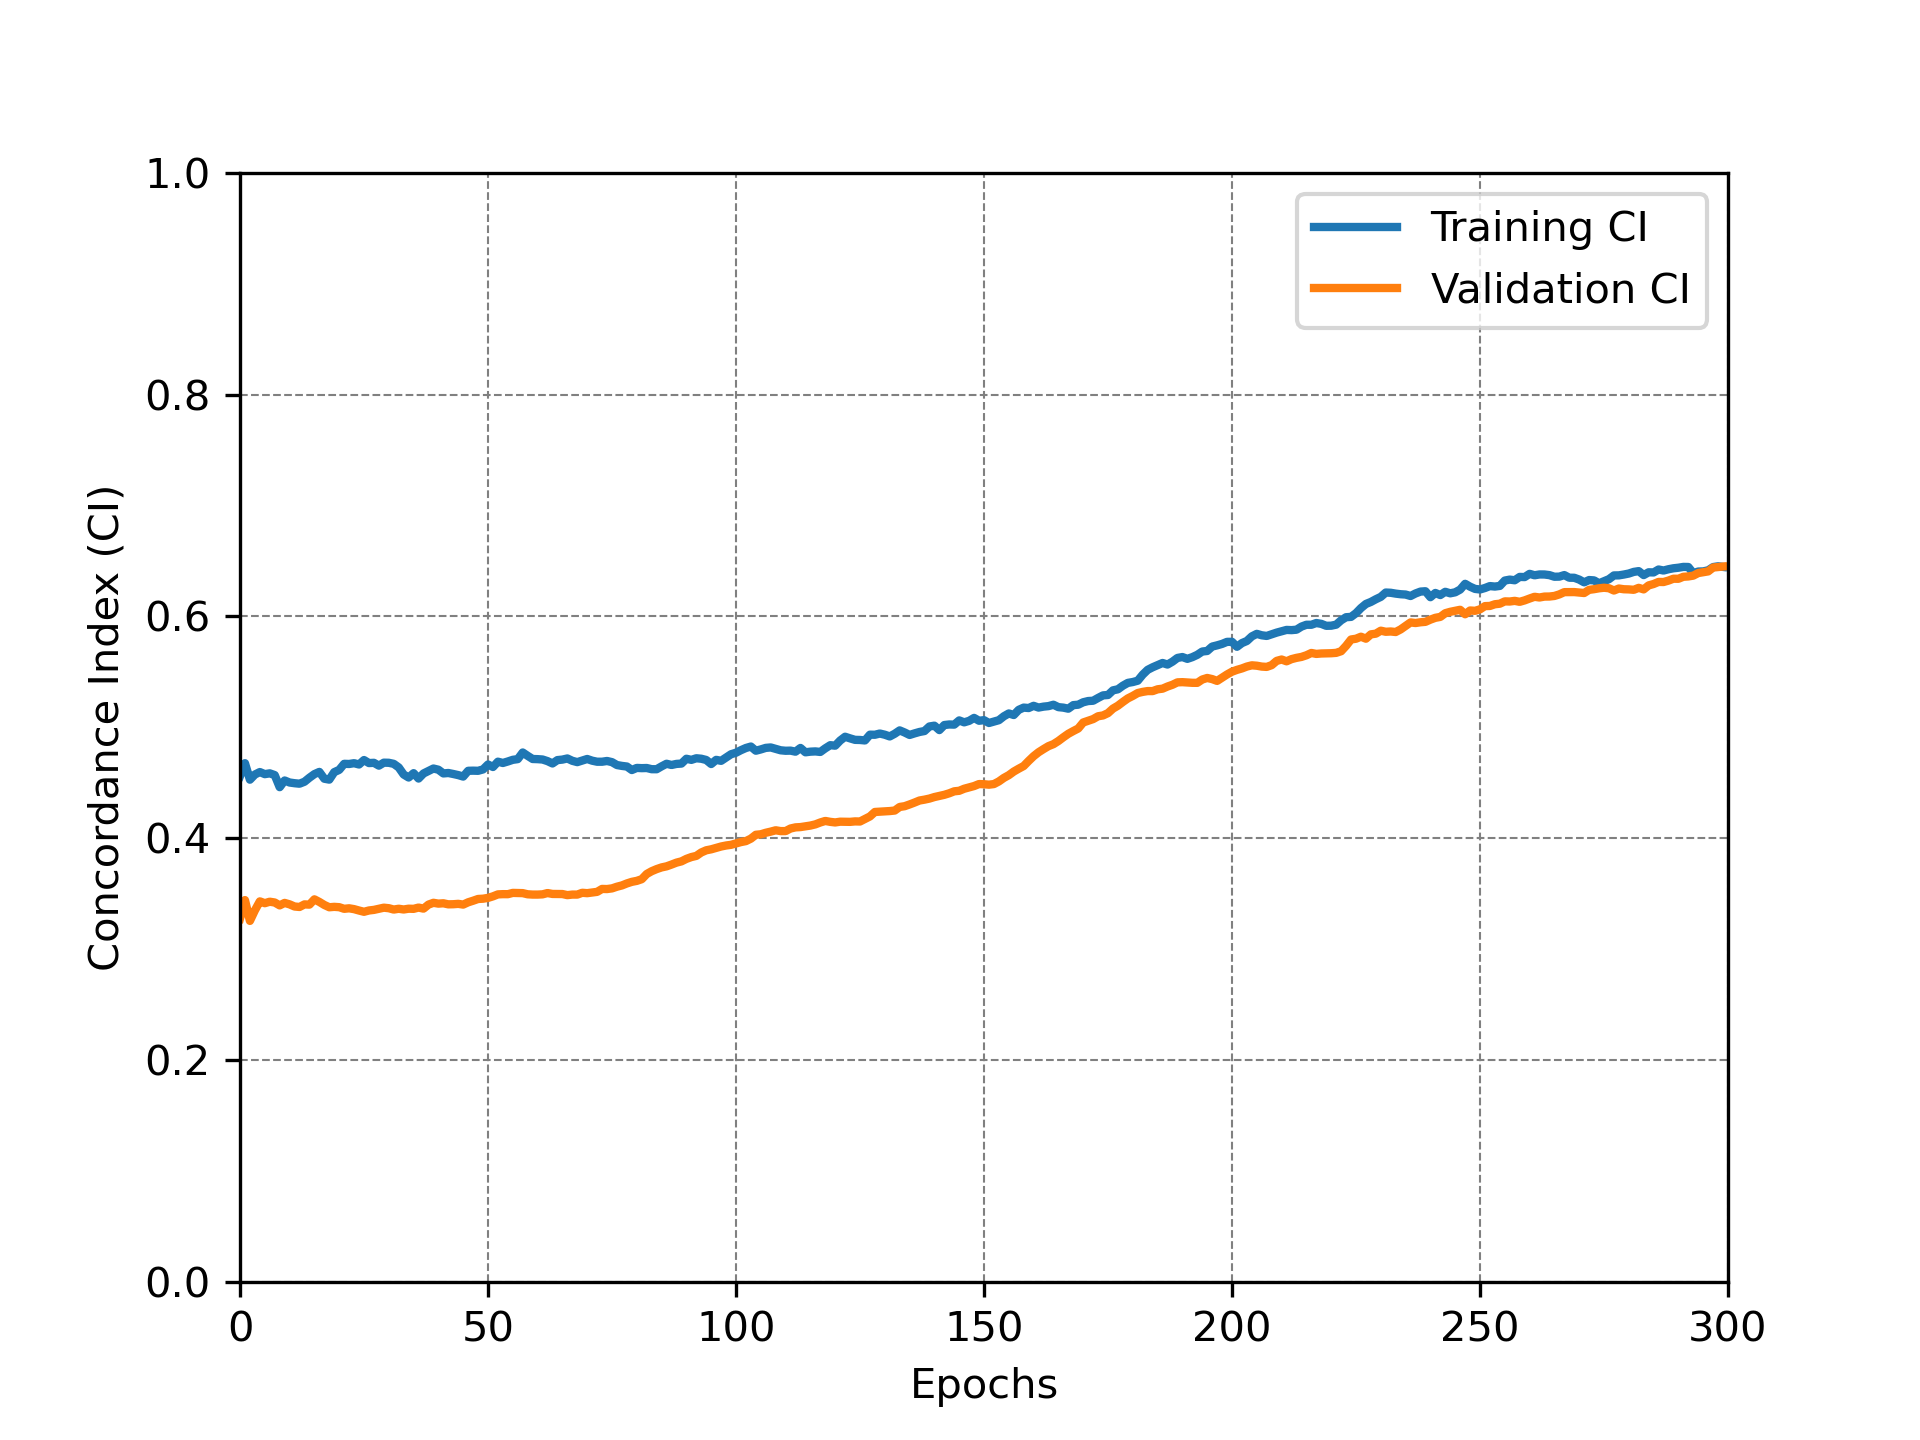
\includegraphics[width=0.49\textwidth]{latex/ci_plots/sum.png}
         \caption{Element-wise summation}
     \end{subfigure}
    \hfill
    \caption[Vector-based Fusion techniques]{Straightforward fusion techniques, that consist of a single vector-vector operation. Losses to the left, and concordance indices to the right.}
    \label{fig:fusions_simple}
\end{figure}

% \clearpage

\begin{figure}[h!b]
        \centering
     \begin{subfigure}[b]{\textwidth}
         \centering
         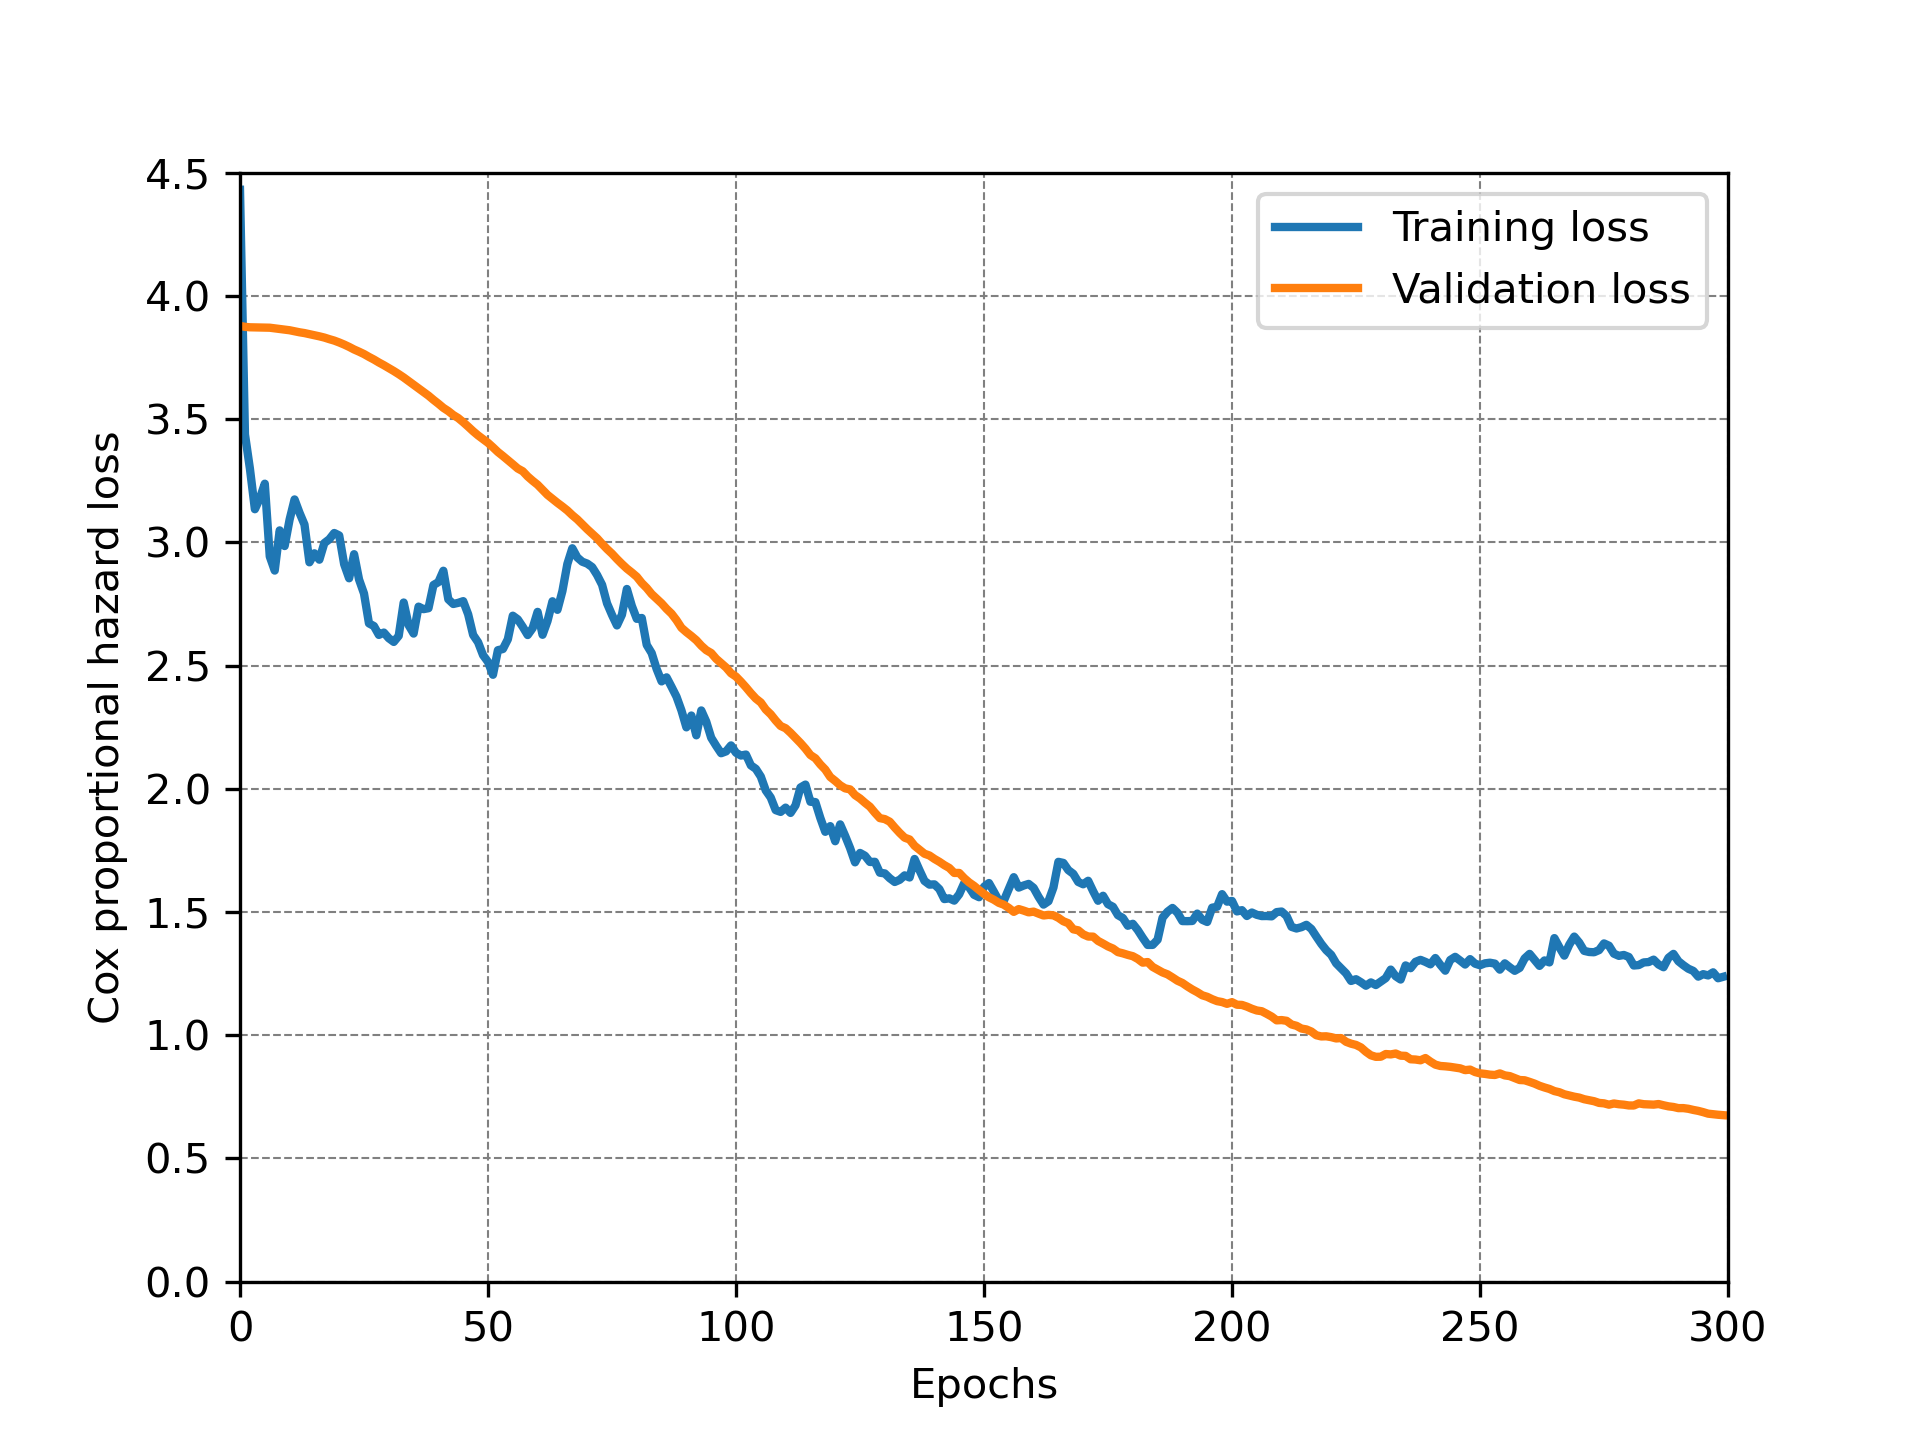
\includegraphics[width=0.49\textwidth]{latex/loss_plots/attention.png}
         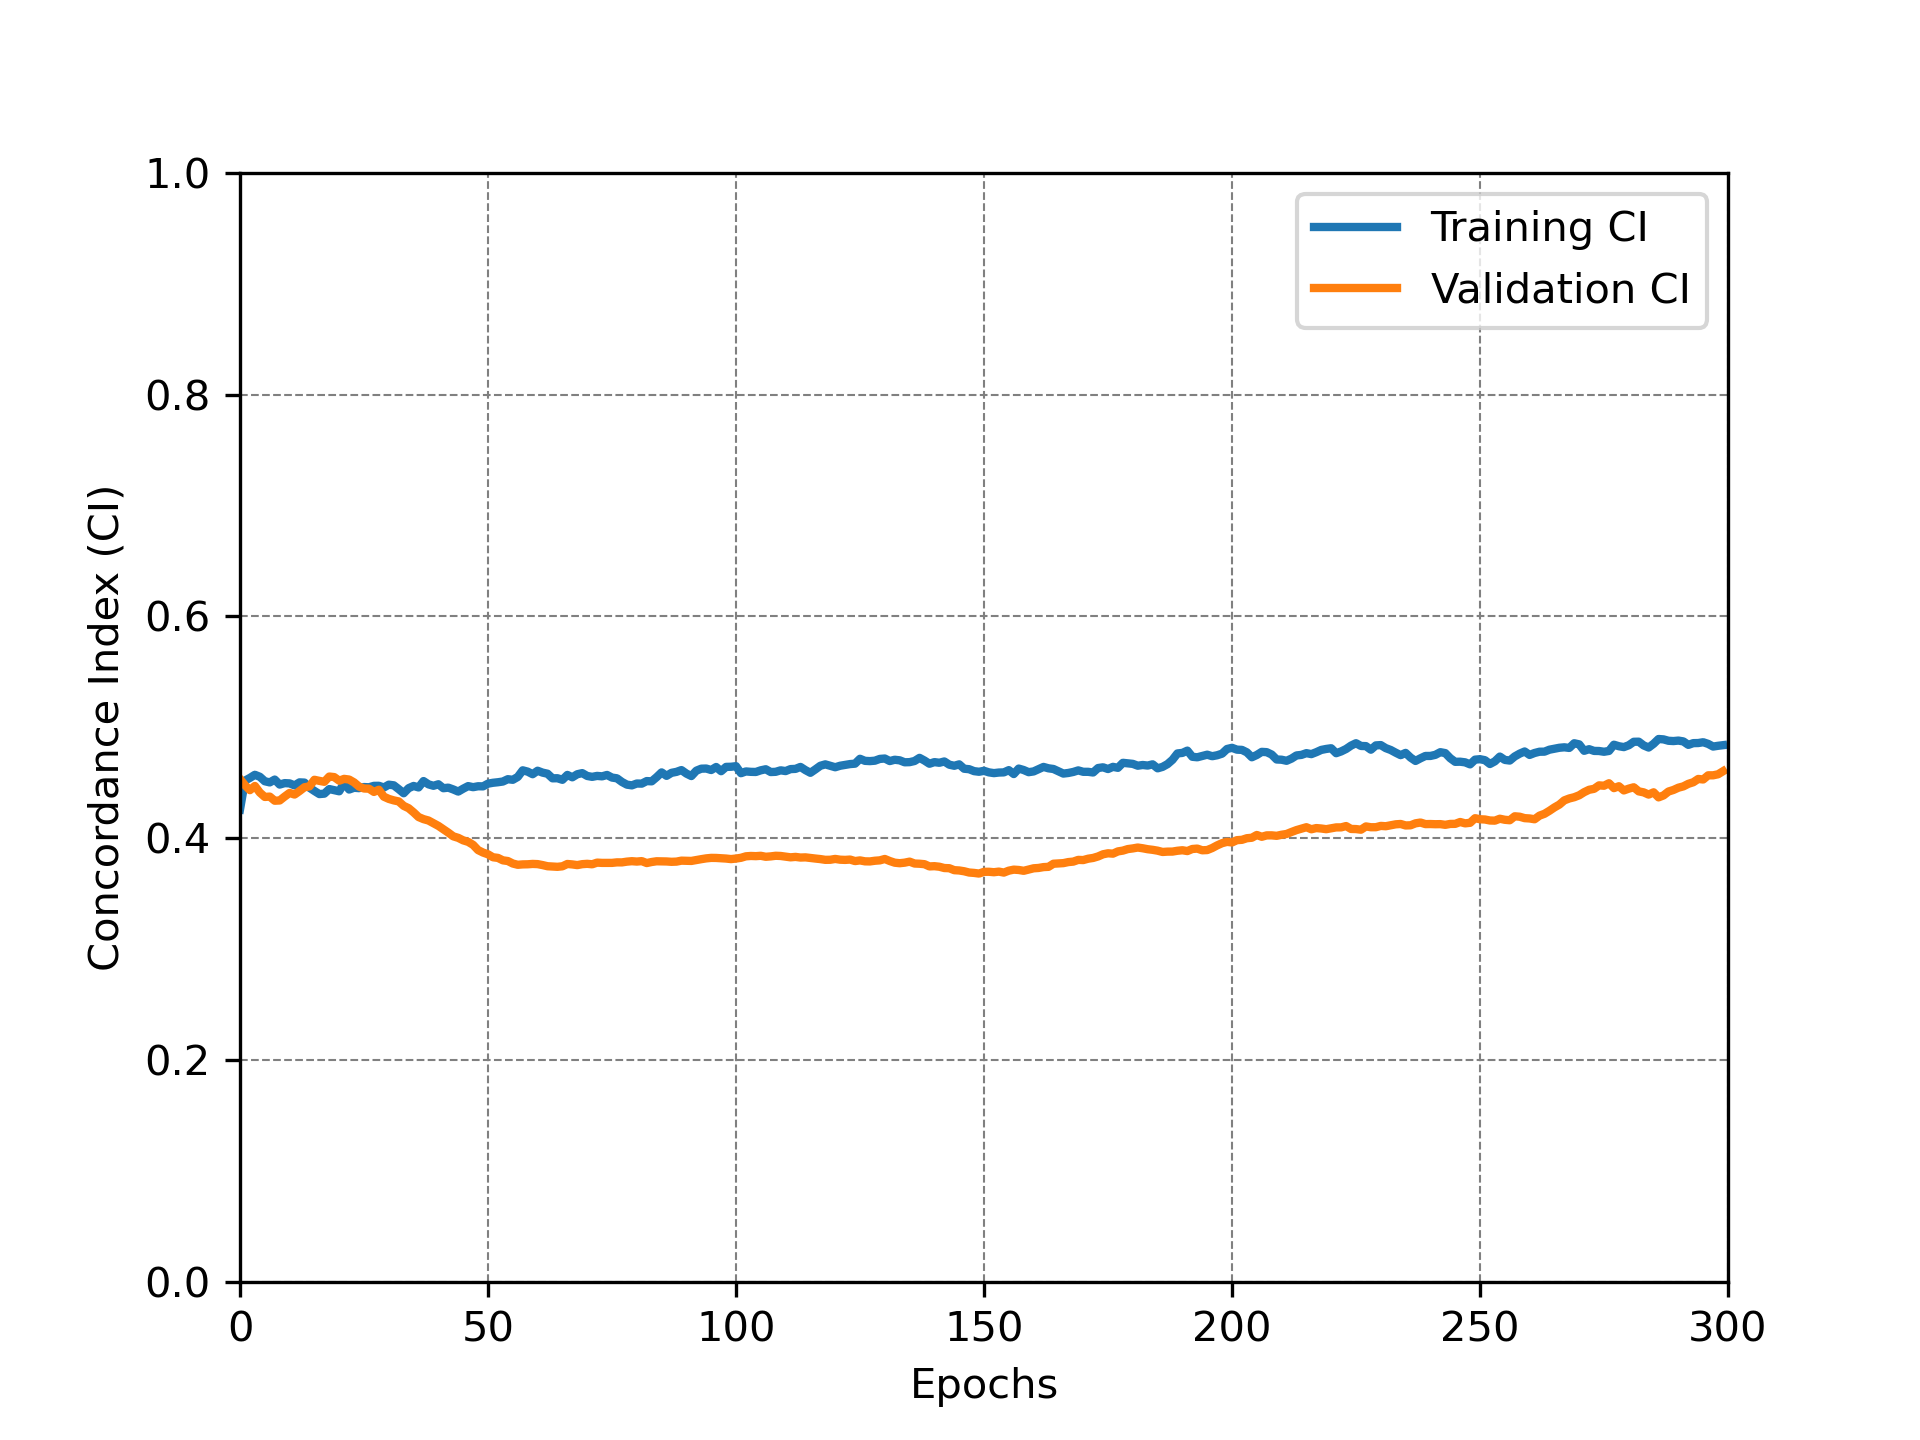
\includegraphics[width=0.49\textwidth]{latex/ci_plots/attention.png}
         \caption{Attention-based}
     \end{subfigure}

\vskip\baselineskip
     \begin{subfigure}[b]{\textwidth}
         \centering
         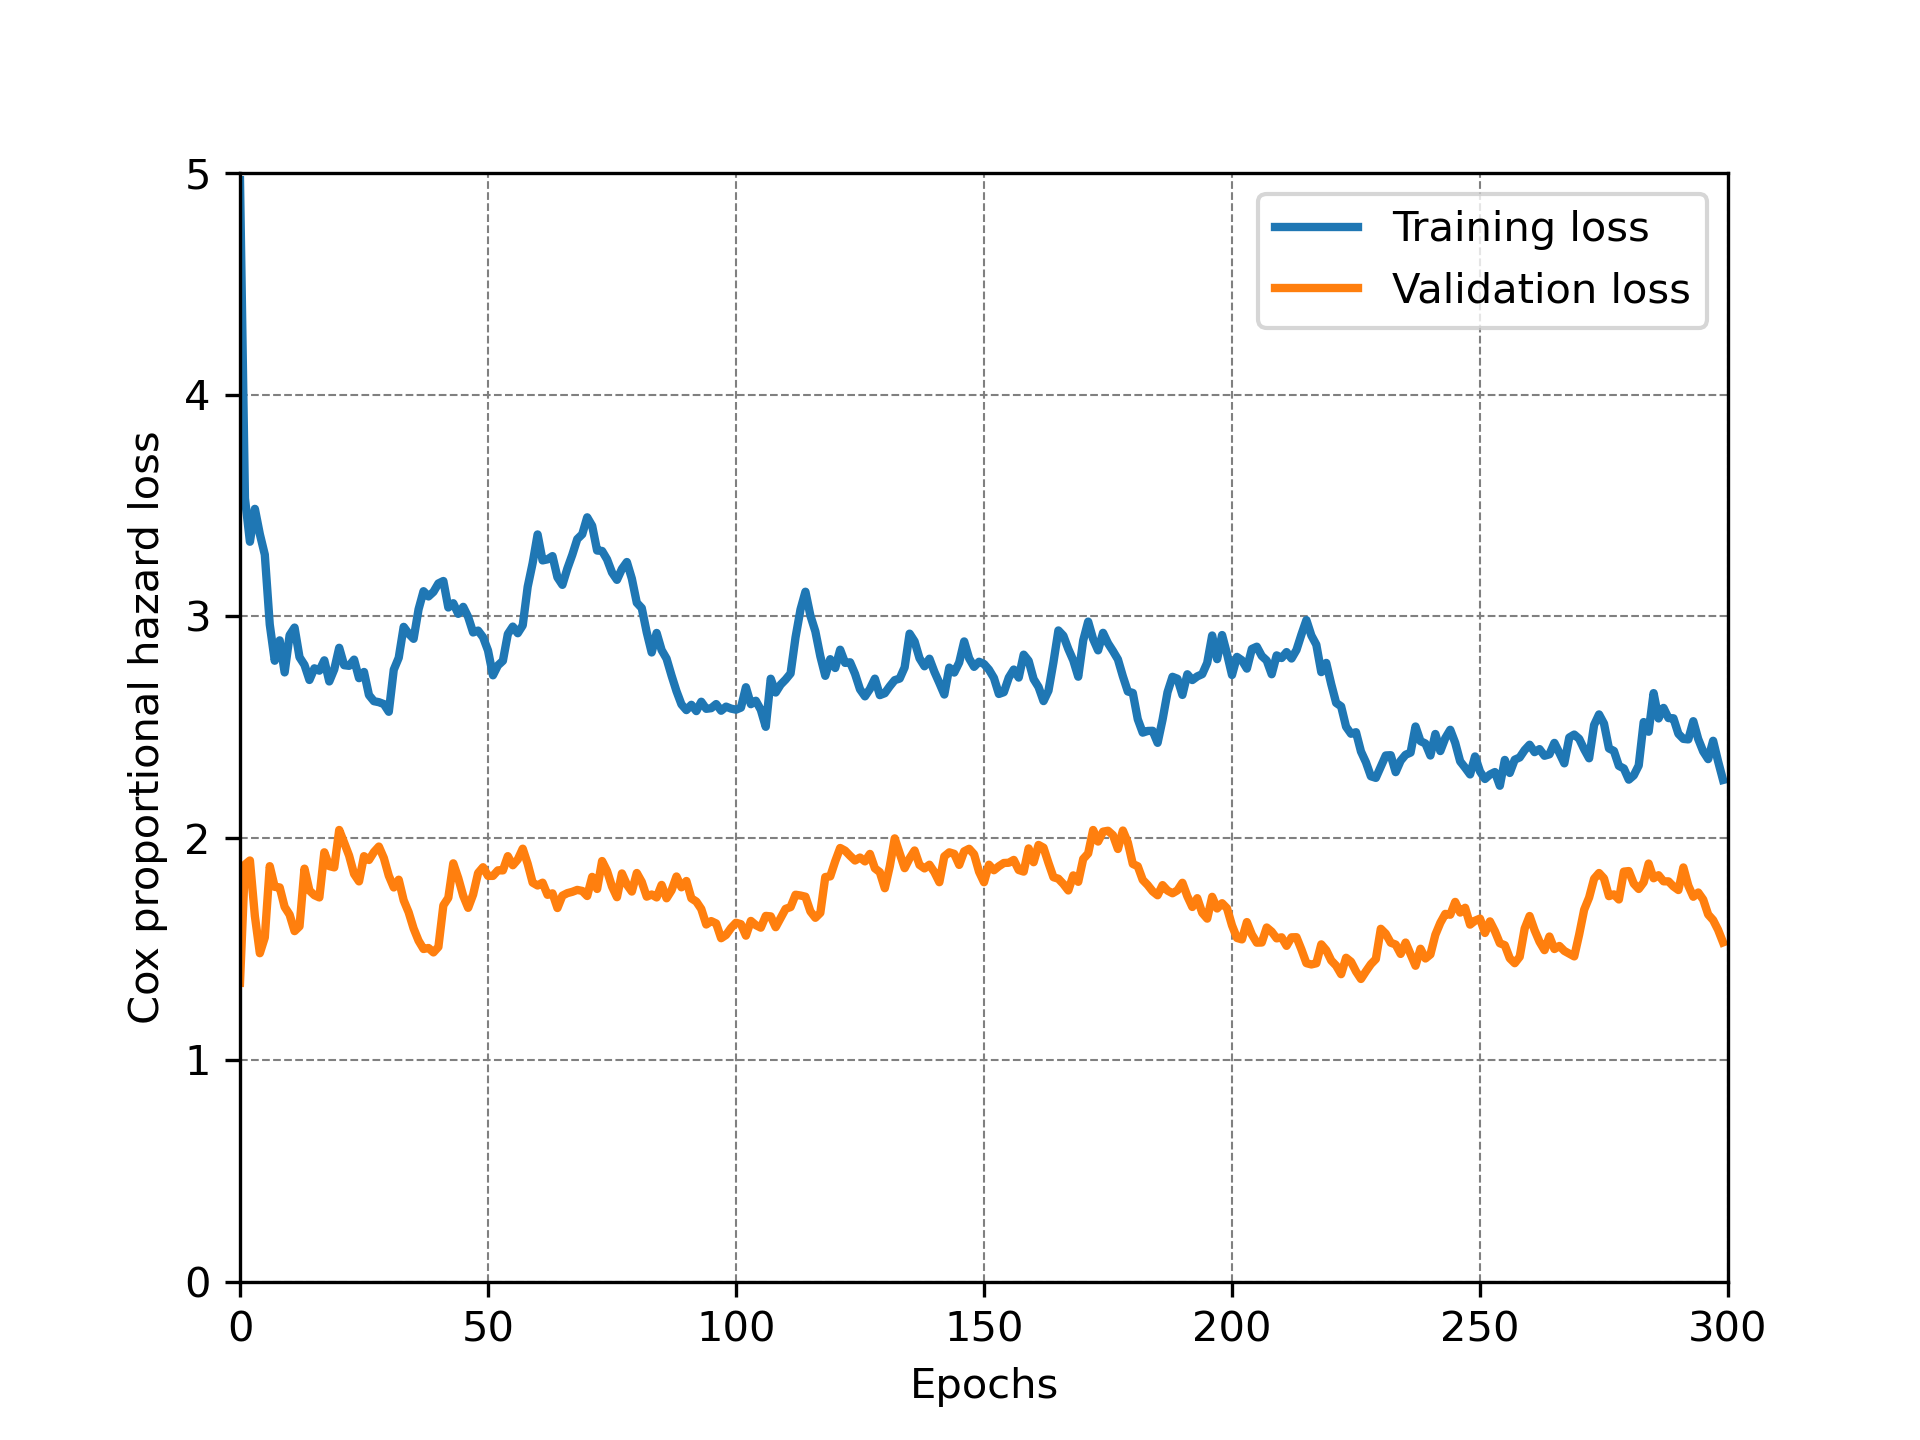
\includegraphics[width=0.49\textwidth]{latex/loss_plots/embrace.png}
         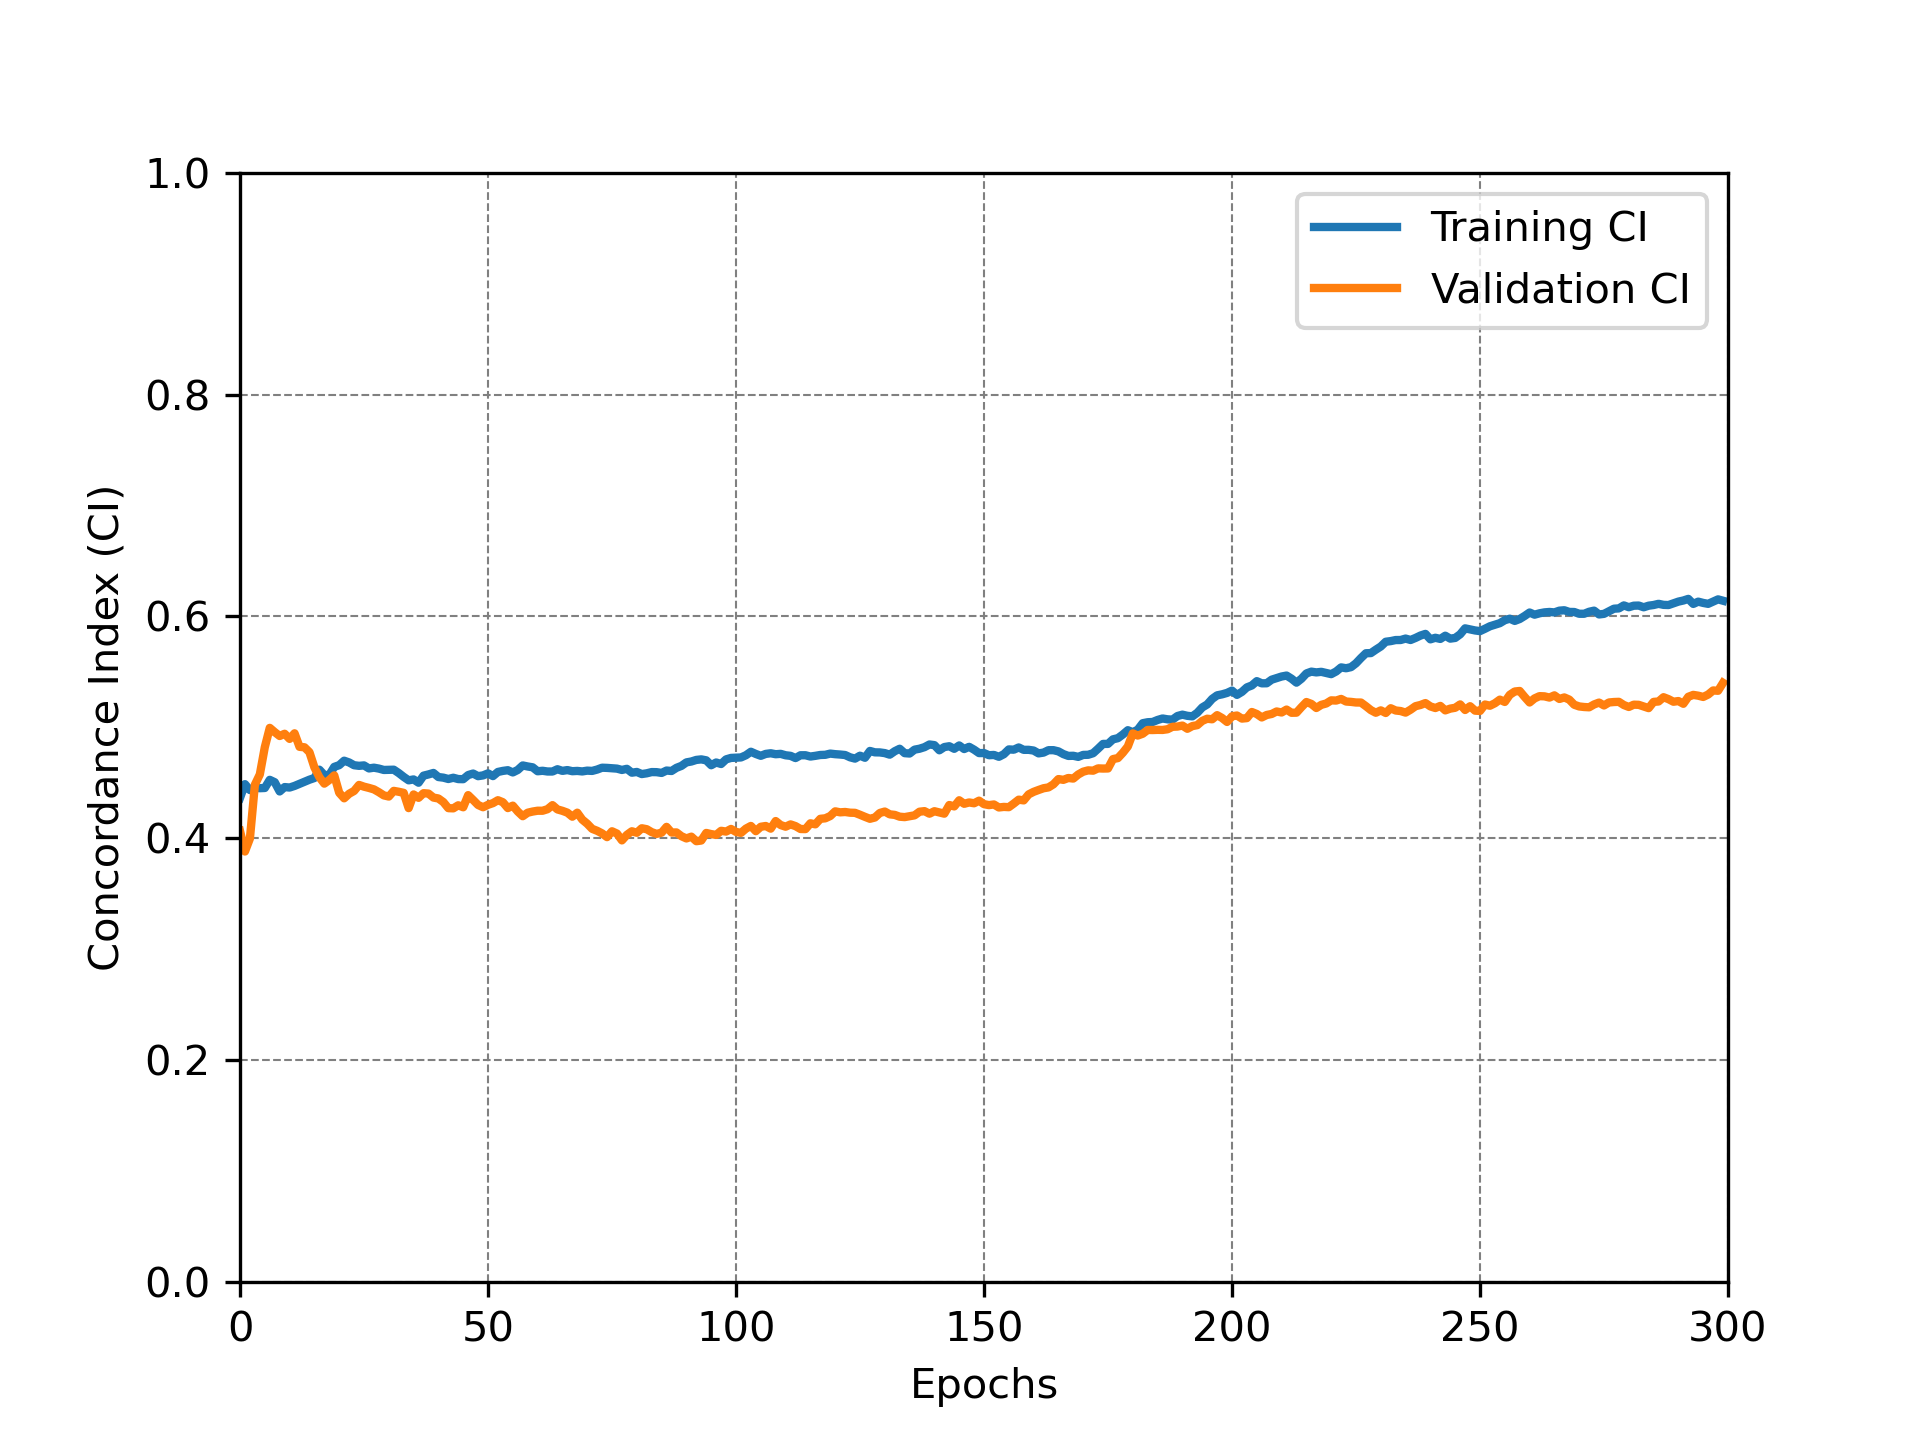
\includegraphics[width=0.49\textwidth]{latex/ci_plots/embrace.png}
         \caption{EmbraceNet}
     \end{subfigure}

\vskip\baselineskip
     \begin{subfigure}[b]{\textwidth}
         \centering
         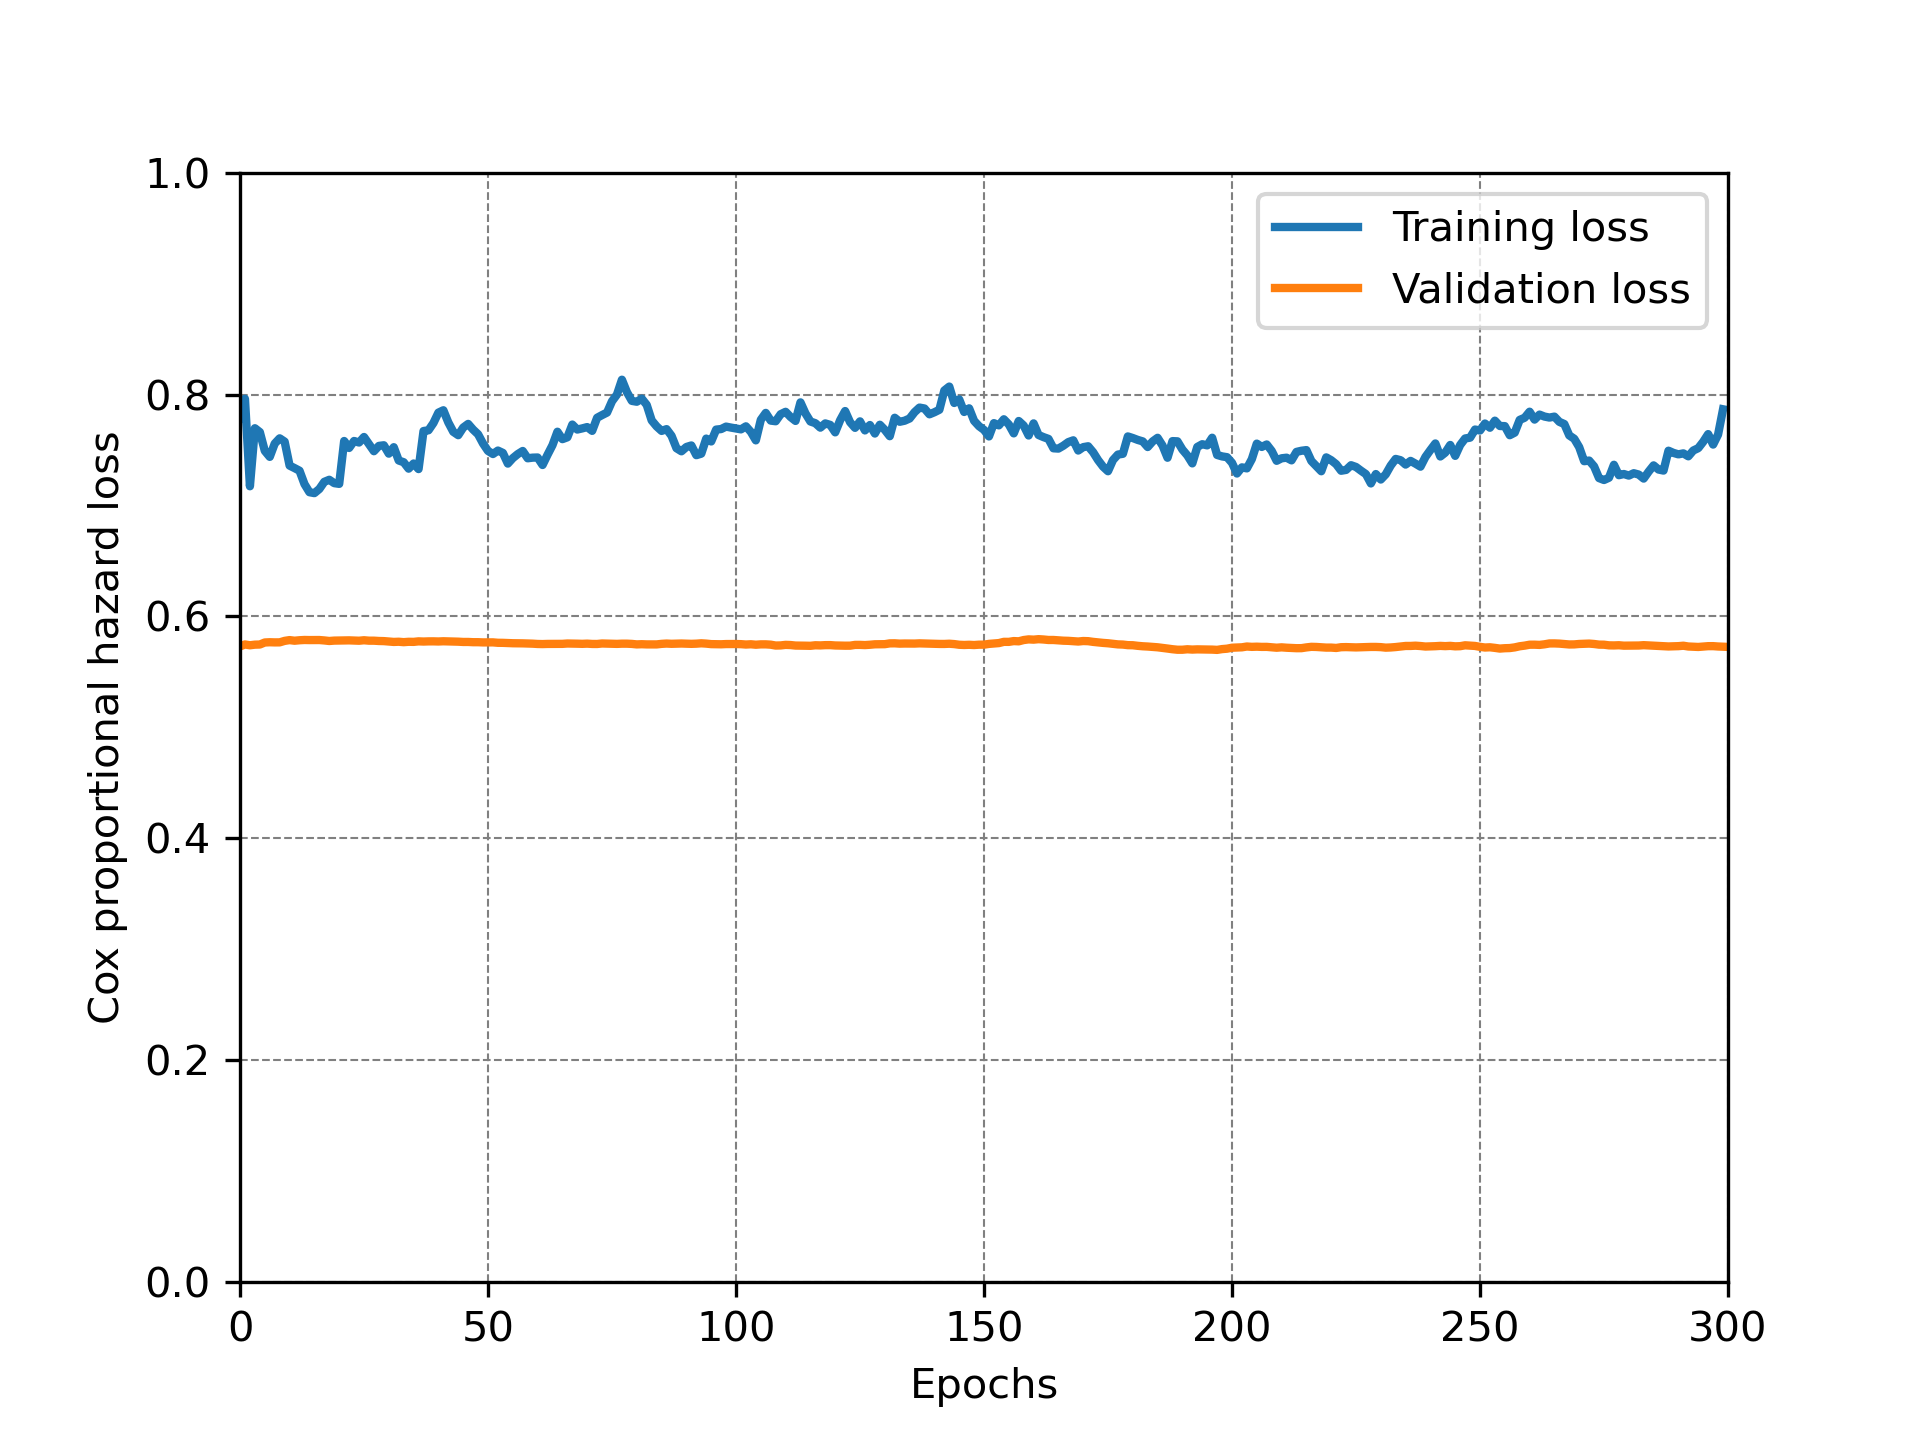
\includegraphics[width=0.49\textwidth]{latex/loss_plots/kronecker.png}
         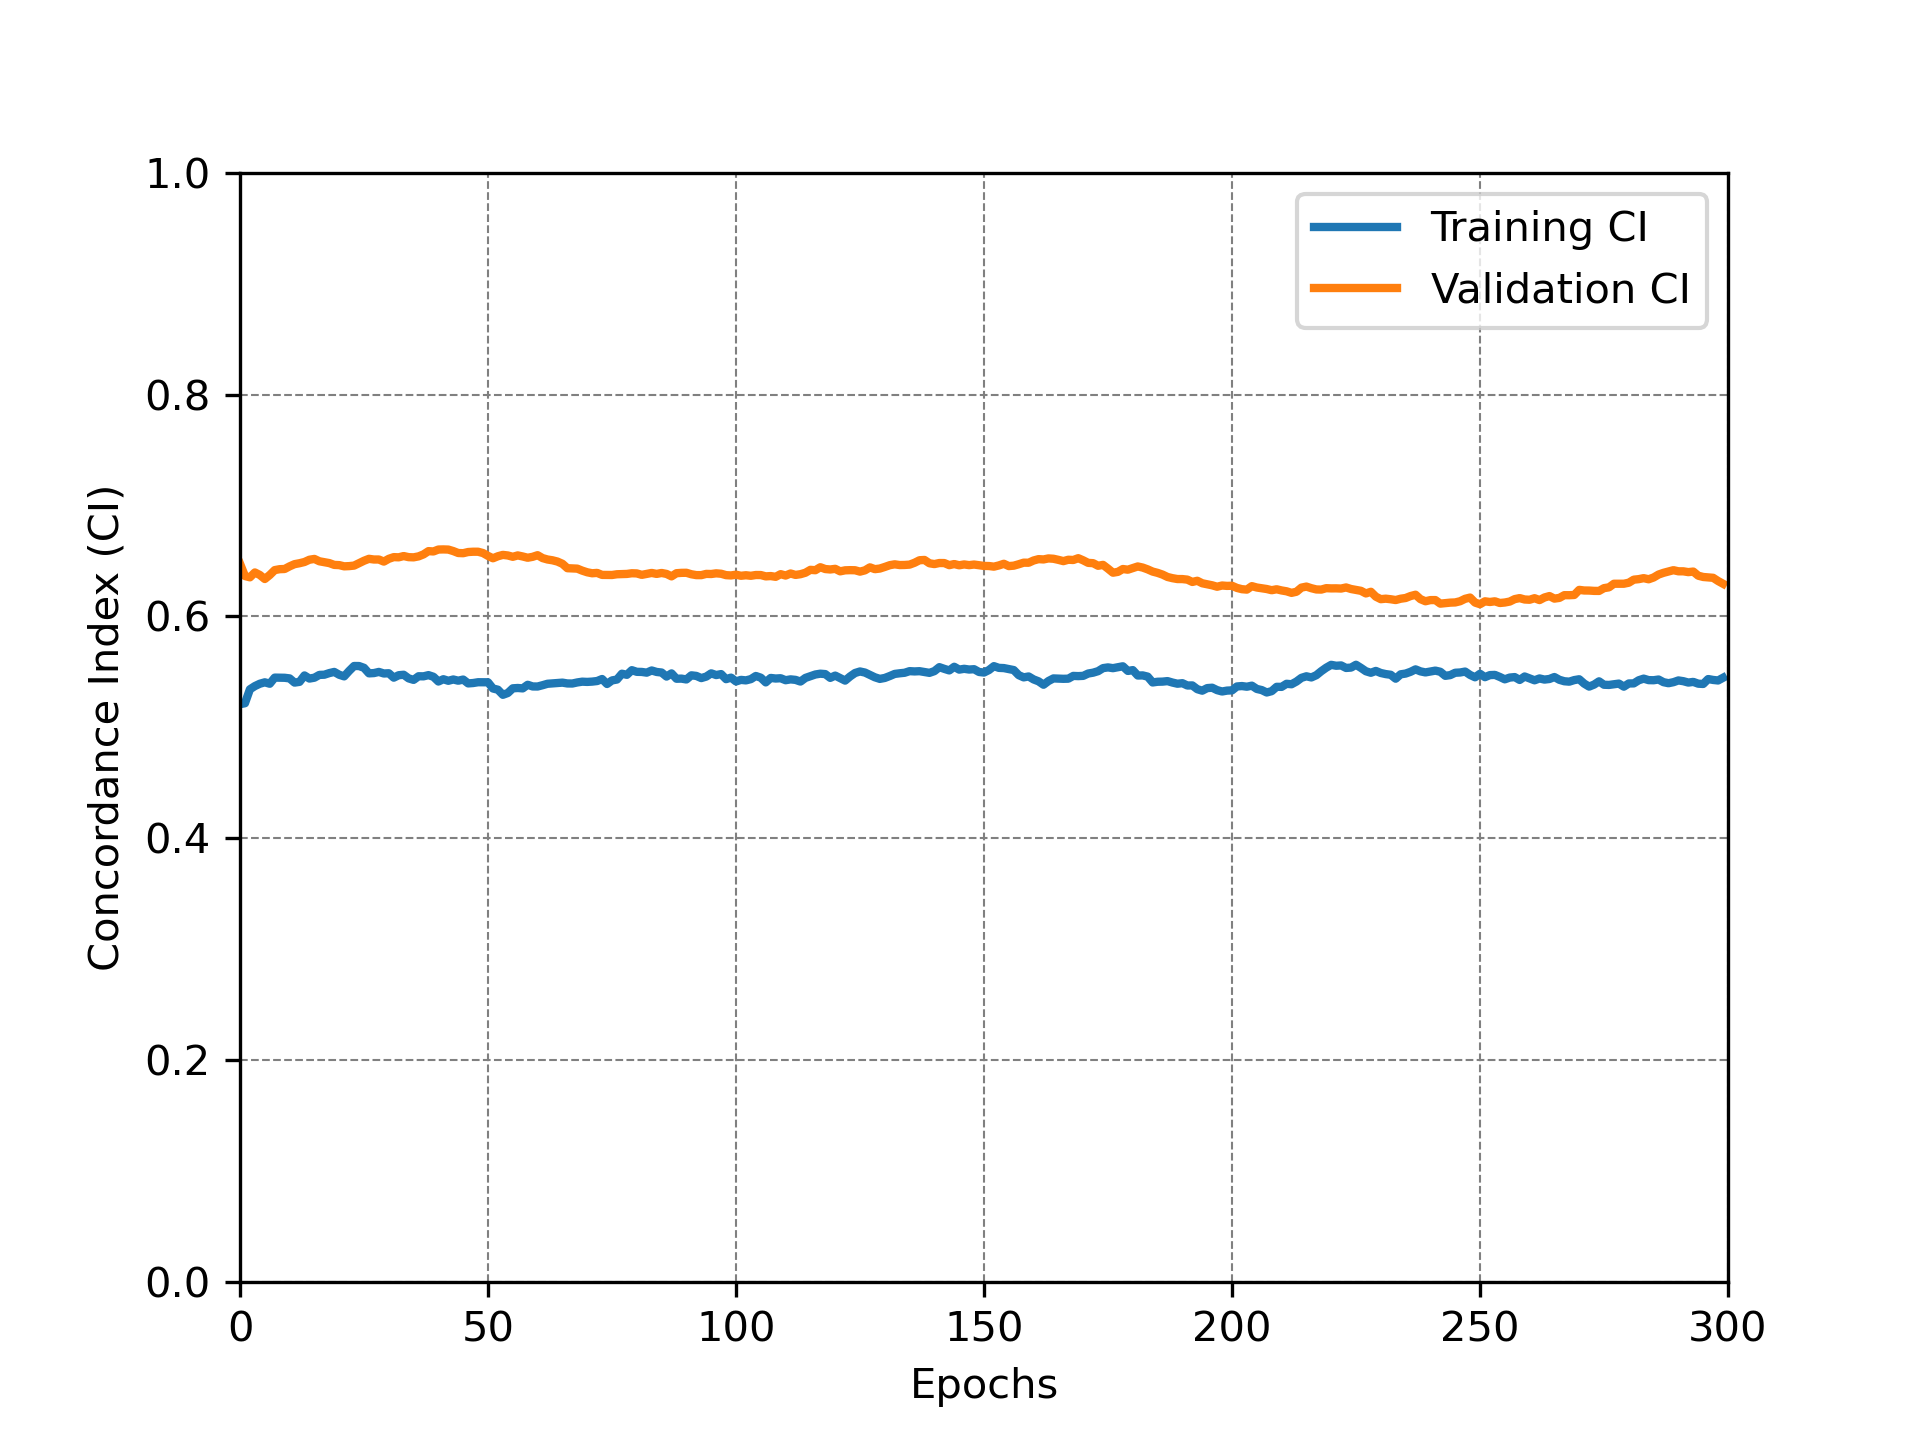
\includegraphics[width=0.49\textwidth]{latex/ci_plots/kronecker.png}
         \caption{Attention-gated Kronecker product}
     \end{subfigure}

    \hfill
    \caption[Complex Fusion techniques]{Complex fusion techniques that involve either stochastic processes or additional hidden layers.}
    \label{fig:fusions_complex}
\end{figure}

%%%%%%%%%%%%%%%%%%%%%%%%%%%%%%%%%%%%%%%%%%%%%%%%%%%%%%%%%%%%%%%%%%%%%%%%%%%%%%%%%%%%%%%%%%%%%%%%%%%%%%%%%%%%%
\clearpage

\section{Interpretability}

The ResNet version of the unimodal model for processing the WSI was used to analyse the feature attribution of the WSI images. Examples of the corresponding results are shown in figures \ref{fig:case111a}, \ref{fig:case111b}, \ref{fig:case13a}, \ref{fig:case13b}, \ref{fig:case13c}, and \ref{fig:case129}. The attributions of the Guided GradCAM method were not converted to absolute values, because the rescaling of values to fit the colour scale would have made interesting aspects appear invisible. 
Integrated Gradients were calculated using 50 intermediate steps. For GradCAM, the last convolutional layer was used to calculate the attribution. As the convolutional layer has much smaller dimensions than the original input image, the results were expected to be more coarse, as can be seen in the figure. 
The occlusion technique uses a kernel of size 8×50×50 with stride of 8×50×50 as well. Saliency and Input*Gradient have no adjustable parameters to be reported. 

All the cases shown here were part of the test set during training. This means that these samples were not used for training nor model evaluation during training. The model used for inference was picked from the training epoch with the highest concordance index on the validation set.

\ref{fig:case129} shows only a selection of applied method, as some results were deemed less interesting. More visualisation in the same manner can be found in Appendix \ref{chap:App2} Figures \ref{fig:case181} and \ref{fig:case121}.

\begin{figure}[h!t]
    \centering
     \begin{subfigure}[b]{0.475\textwidth}
         \centering
         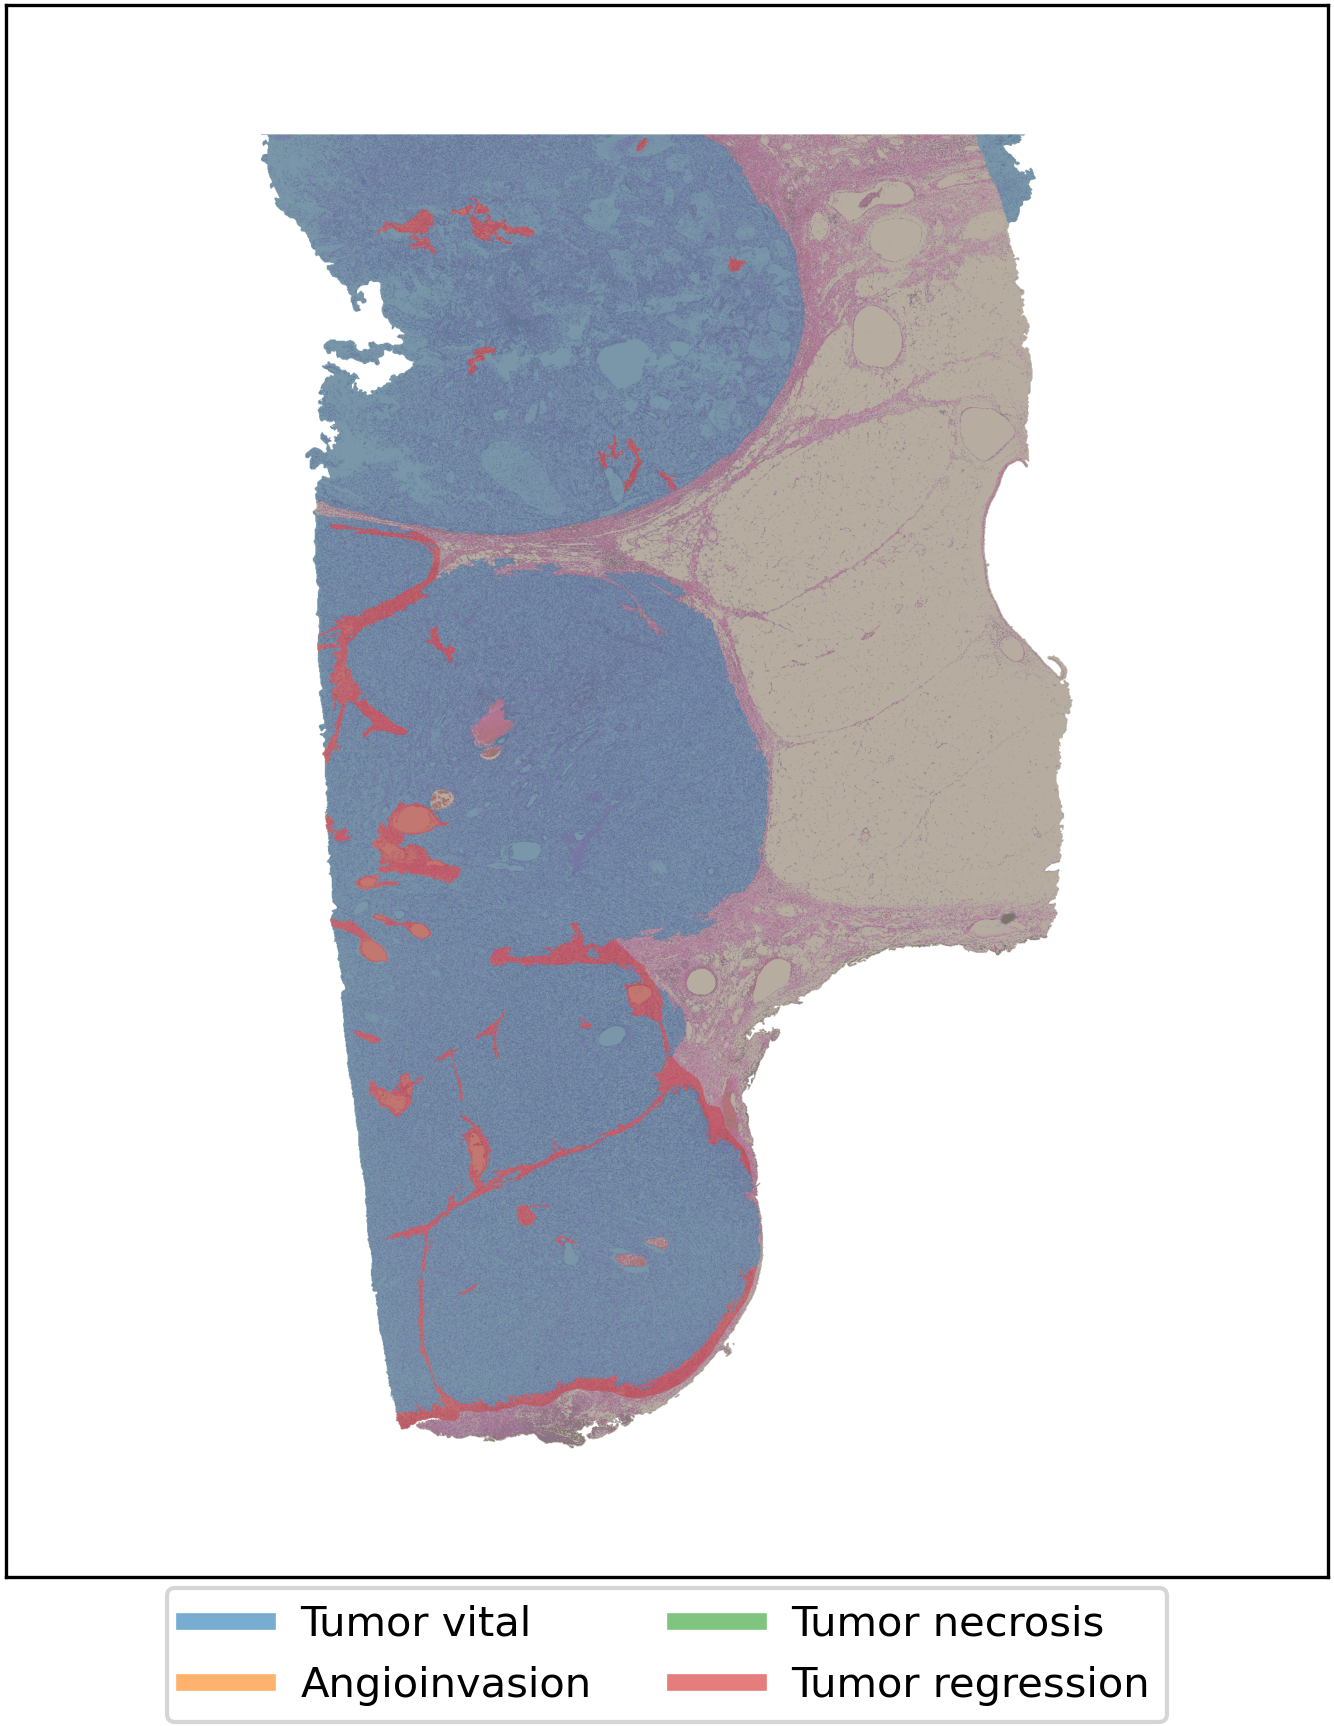
\includegraphics[width=\textwidth]{latex/captum/case111/masks_case111-stain1-censored_3499days.png}
         \caption{Tumour annotations of WSI}
     \end{subfigure}
    \hfill
     \begin{subfigure}[b]{0.49\textwidth}
         \centering
         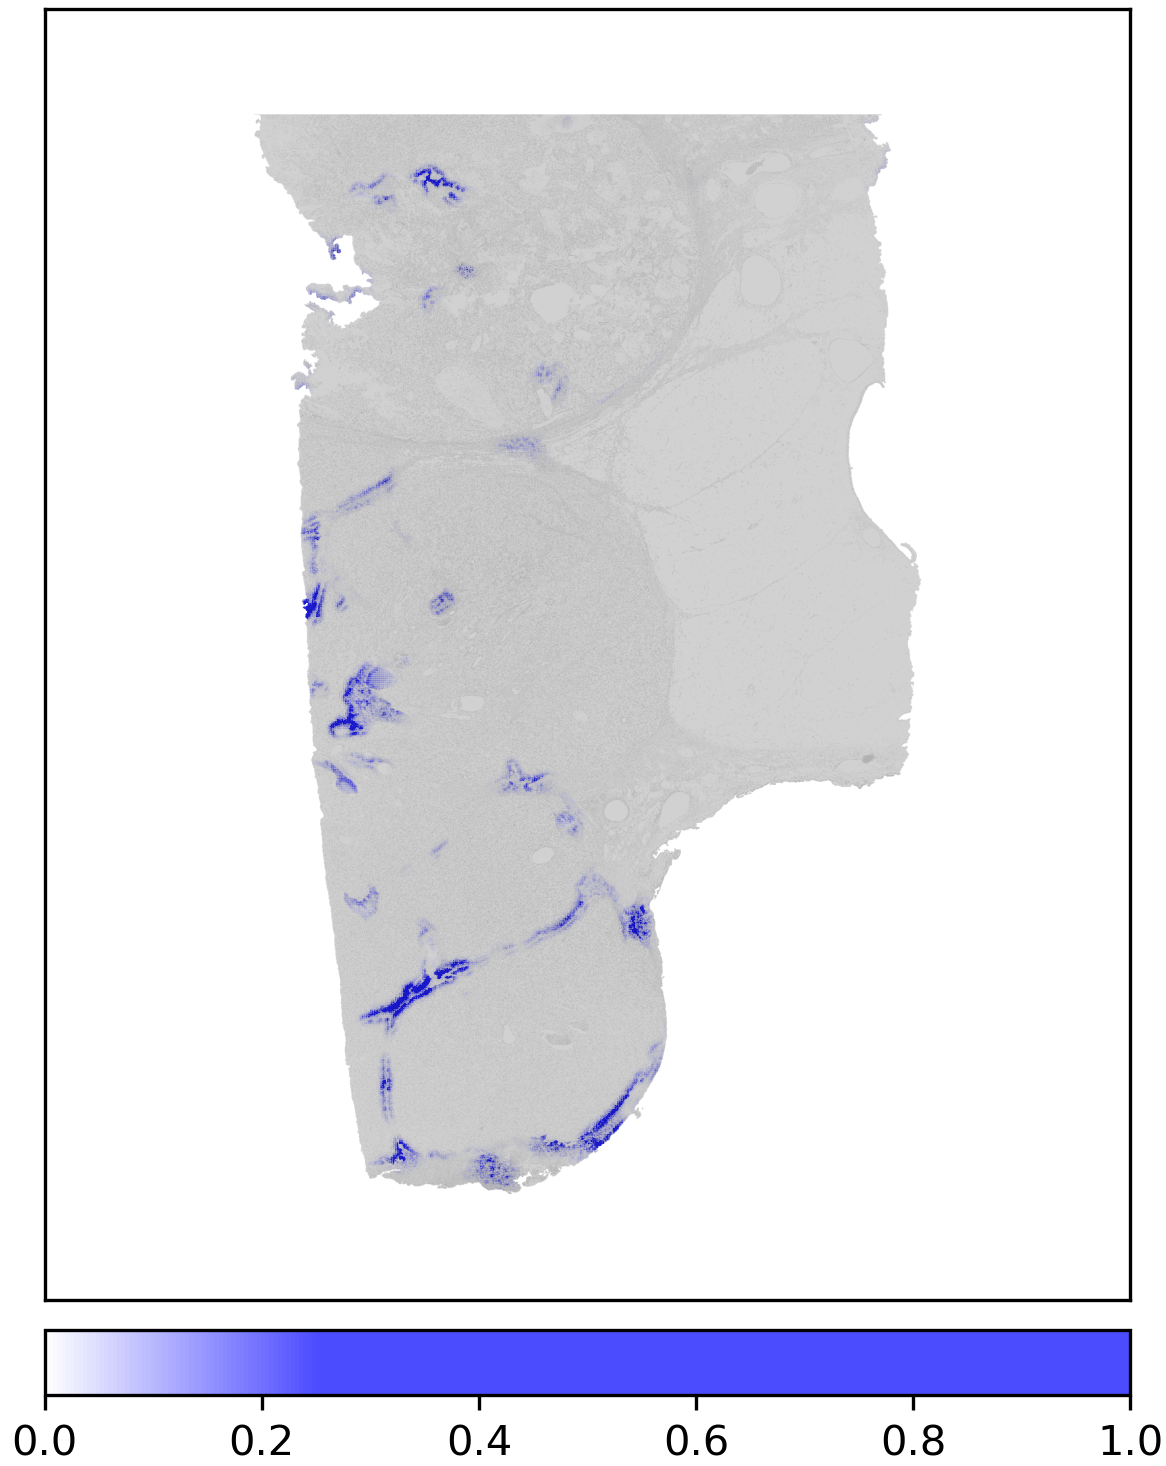
\includegraphics[width=\textwidth]{latex/captum/case111/integrated_gradients_abs_case111-stain1-censored_3499days.png}
         \caption{Integrated Gradients, abs. attributions}
     \end{subfigure}
\vskip\baselineskip
     \begin{subfigure}[b]{0.49\textwidth}
         \centering
         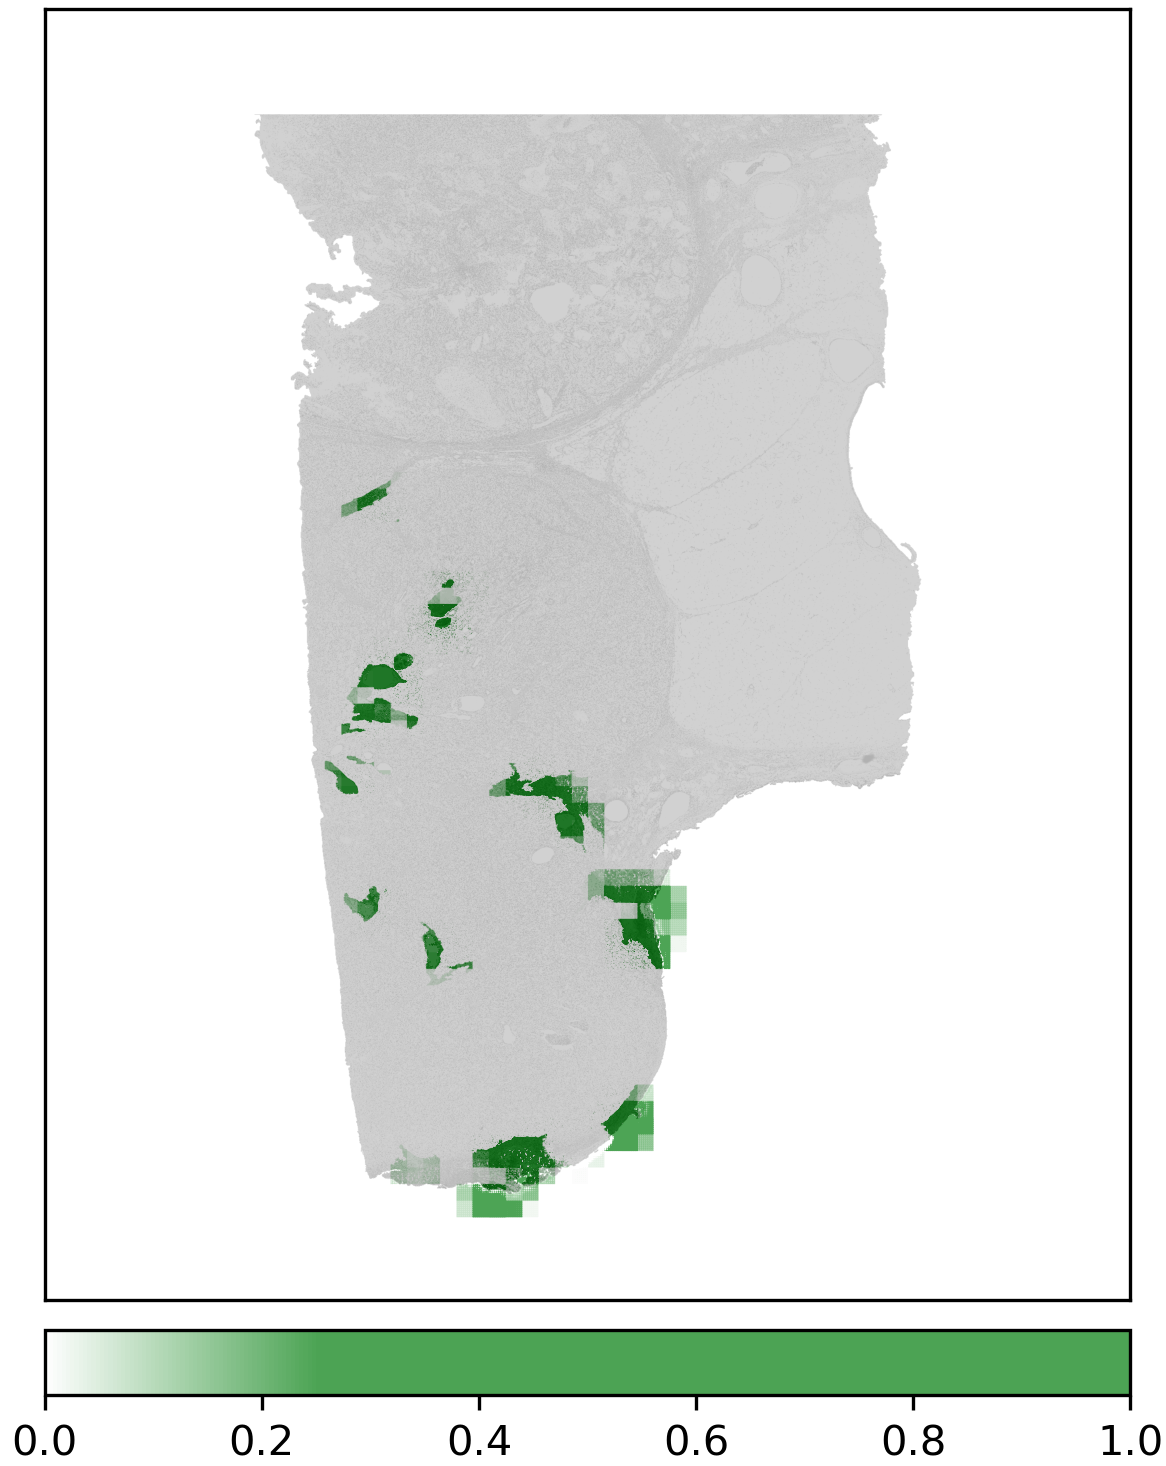
\includegraphics[width=\textwidth]{latex/captum/case111/guided_gradcam_pos_case111-stain1-censored_3499days.png}
         \caption{Guided GradCAM, positive attributions}
     \end{subfigure}
    \hfill
     \begin{subfigure}[b]{0.49\textwidth}
         \centering
         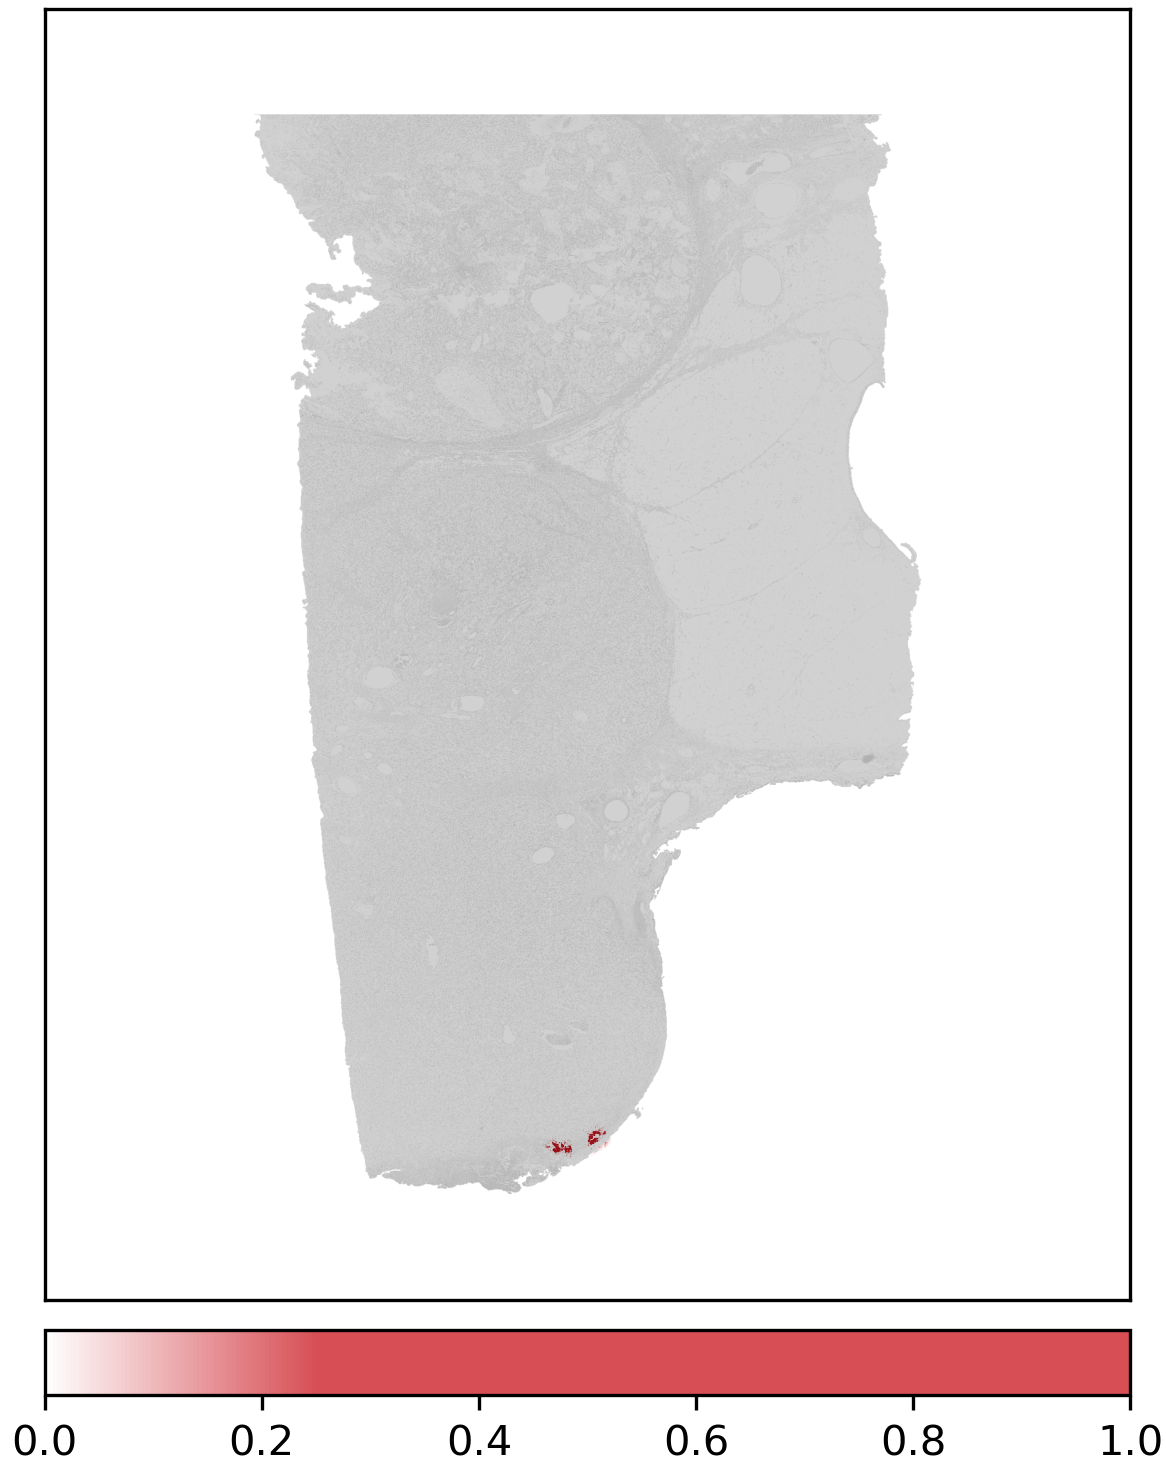
\includegraphics[width=\textwidth]{latex/captum/case111/guided_gradcam_neg_case111-stain1-censored_3499days.png}
         \caption{Guided GradCAM, negative attributions}
     \end{subfigure}
    \hfill
    \caption[Integrated gradients and Guided GradCAM for case 111]{Results of Integrated Gradients and Guided GradCAM for case 111. The figure of the tumour masks is included for comparison. Integrated Gradients attributions are converted to absolute values.}
    \label{fig:case111a}
\end{figure}


\begin{figure}[h!t]
    \centering
     \begin{subfigure}[b]{0.475\textwidth}
         \centering
         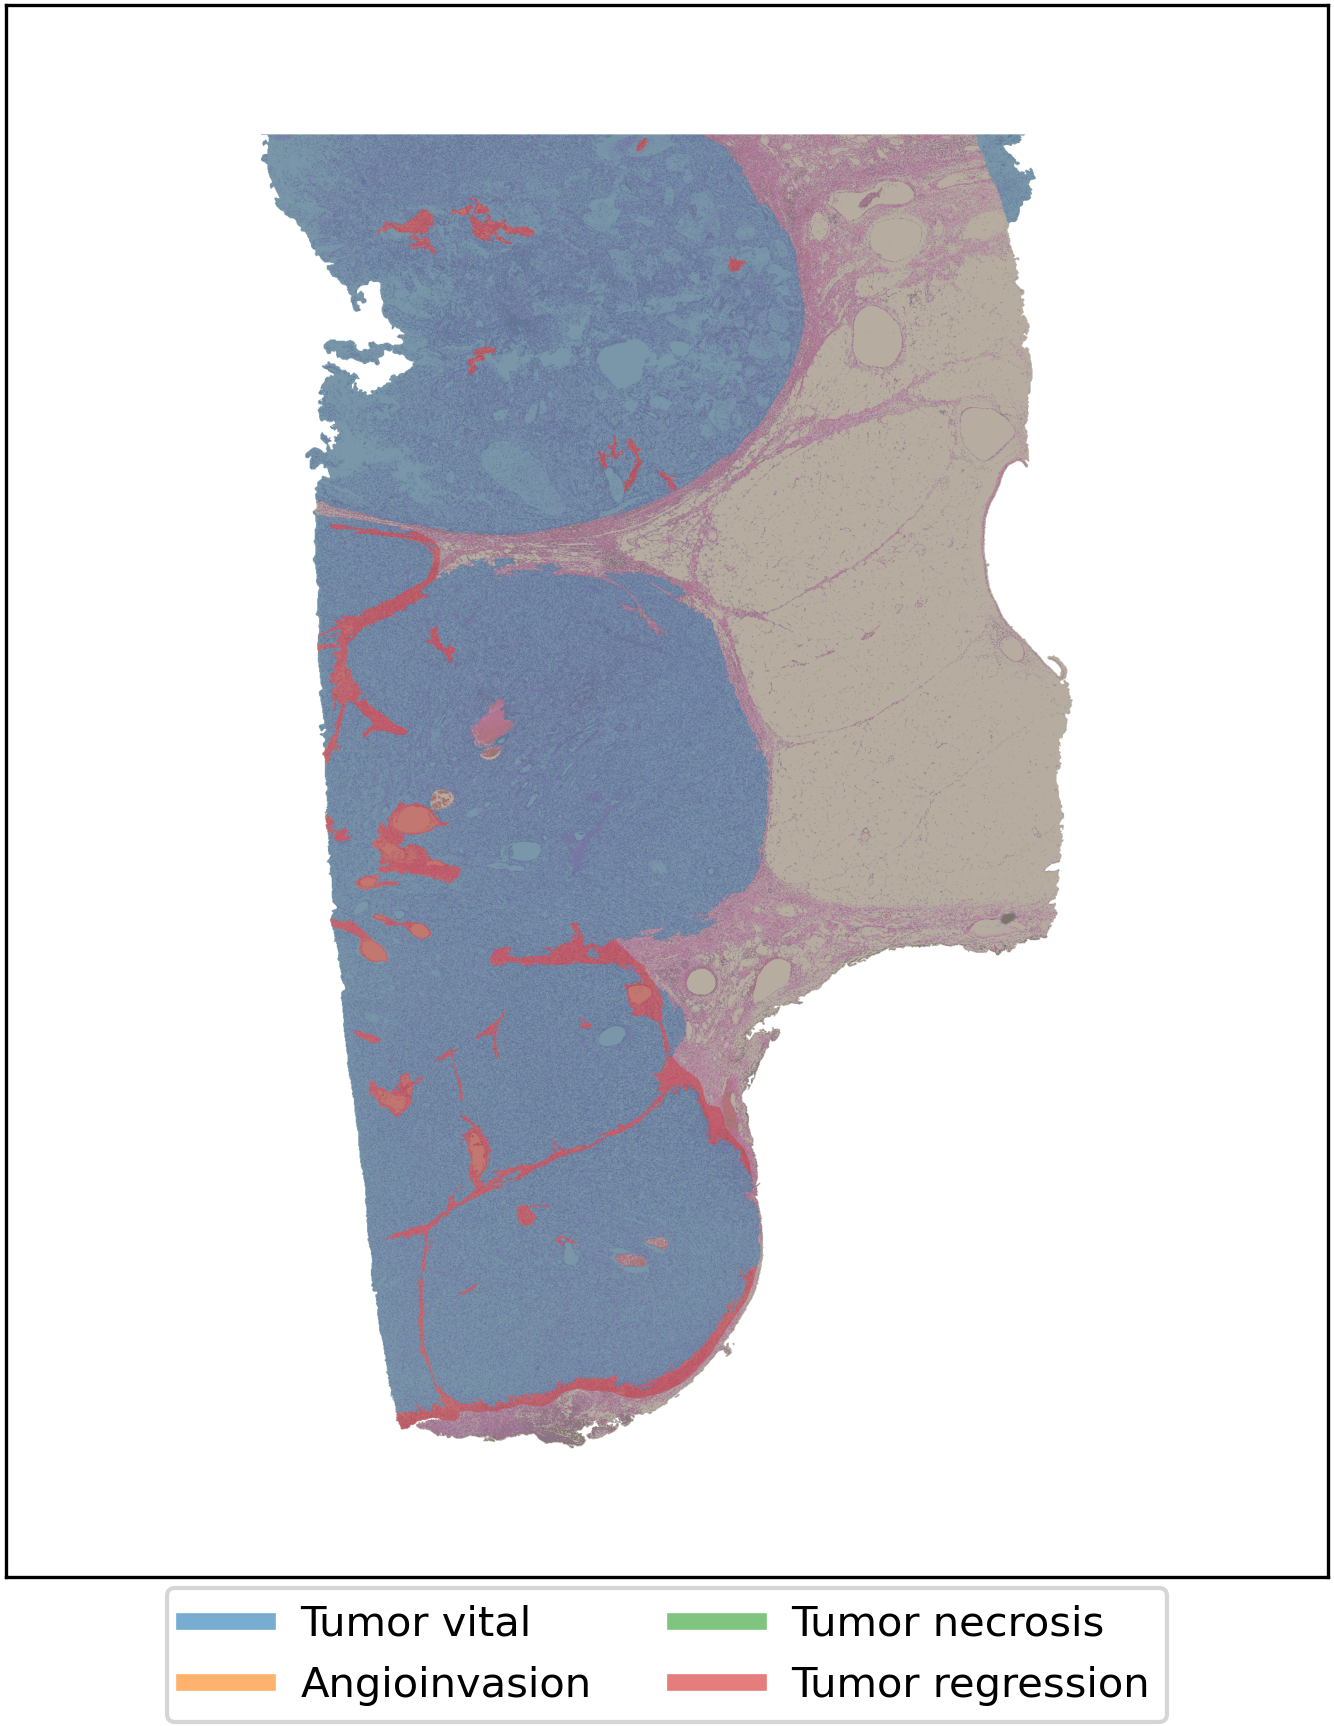
\includegraphics[width=\textwidth]{latex/captum/case111/masks_case111-stain1-censored_3499days.png}
         \caption{Tumour annotations of WSI}
     \end{subfigure}
    \hfill
     \begin{subfigure}[b]{0.49\textwidth}
         \centering
         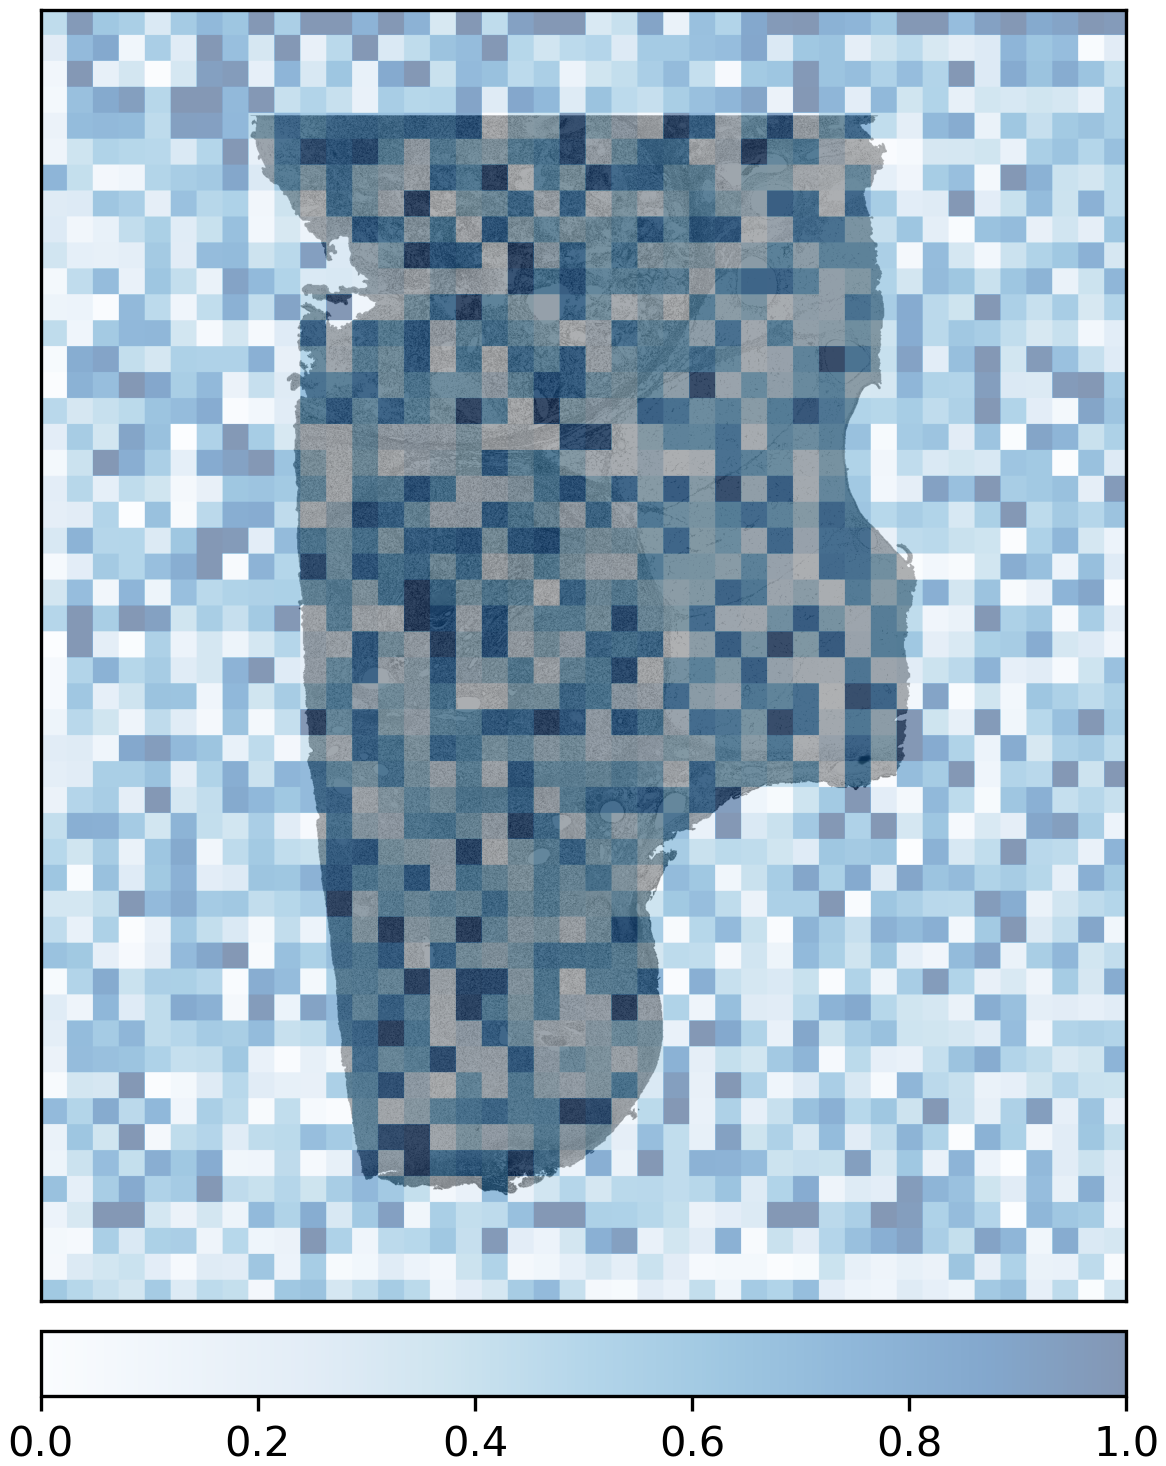
\includegraphics[width=\textwidth]{latex/captum/case111/Occlusion_abs_case111-stain1-censored_3499days.png}
         \caption{Occlusion map; kernel and stride of 50}
     \end{subfigure}
\vskip\baselineskip
     \begin{subfigure}[b]{0.49\textwidth}
         \centering
         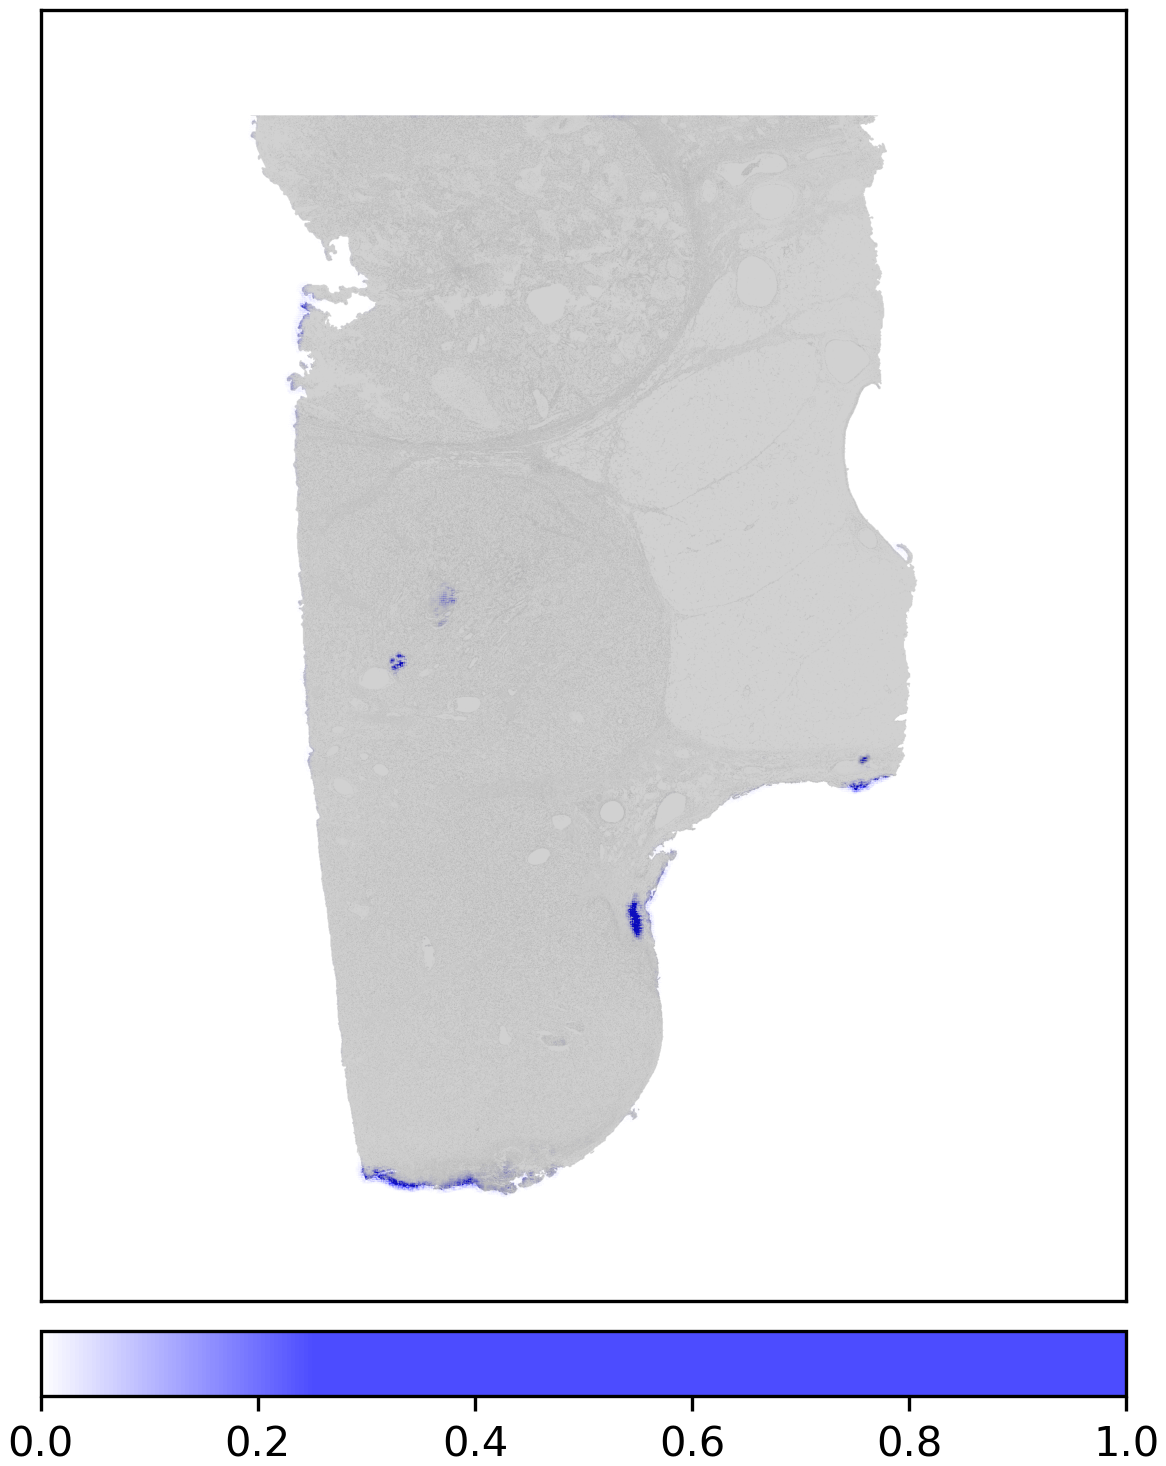
\includegraphics[width=\textwidth]{latex/captum/case111/saliency_case111-stain1-censored_3499days.png}
         \caption{Saliency Maps}
     \end{subfigure}
    \hfill
     \begin{subfigure}[b]{0.49\textwidth}
         \centering
         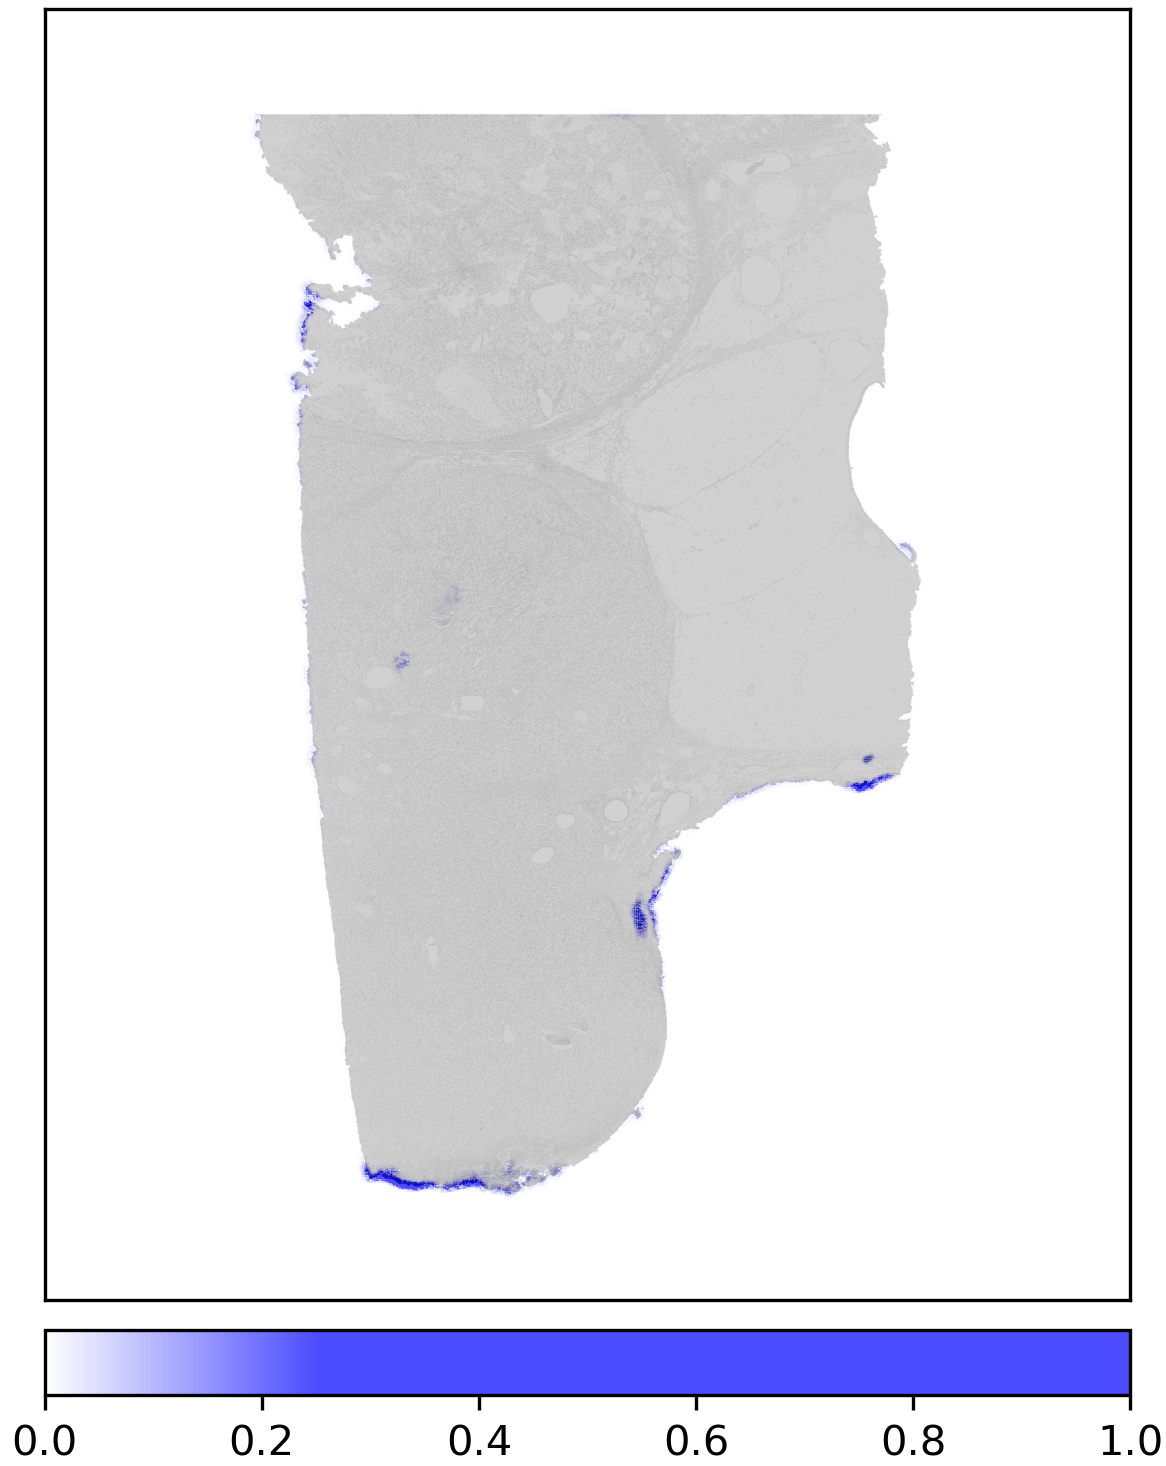
\includegraphics[width=\textwidth]{latex/captum/case111/inputXgradient_pos_case111-stain1-censored_3499days.png}
         \caption{Input*Gradient}
     \end{subfigure}
  
    \hfill
    \caption[Occlusion and Saliency for case 111]{Results of Saliency, Input*Gradients and occlusion mapping for case 111. The figure of the tumour masks is included for comparison. All attributions were converted to absolute values.}
    \label{fig:case111b}
\end{figure}


\begin{figure}[h!t]
    \centering
     \begin{subfigure}[b]{0.475\textwidth}
         \centering
         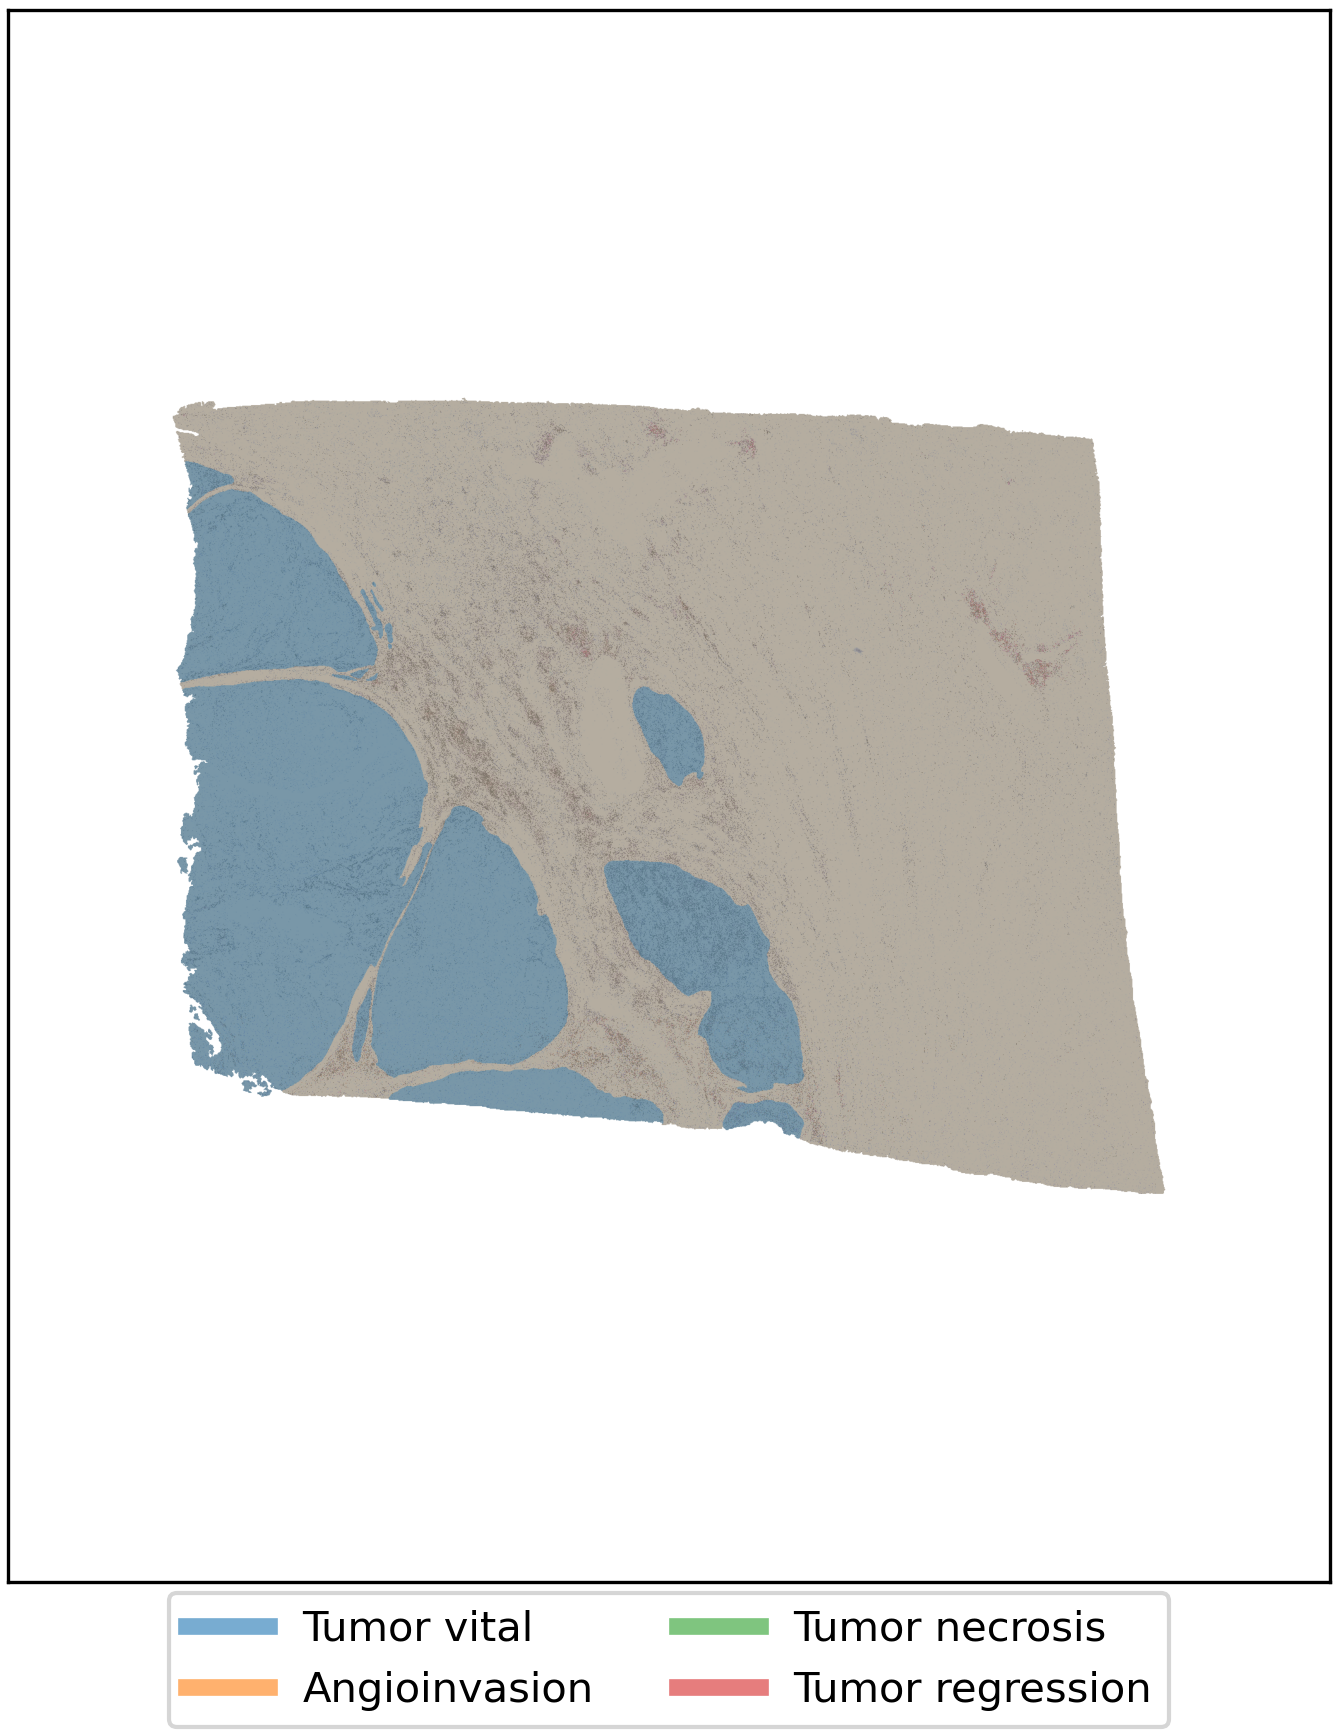
\includegraphics[width=\textwidth]{latex/captum/case13/masks_case13-stain41-dead_2415days.png}
         \caption{Tumour annotations of WSI}
     \end{subfigure}
    \hfill
     \begin{subfigure}[b]{0.49\textwidth}
         \centering
         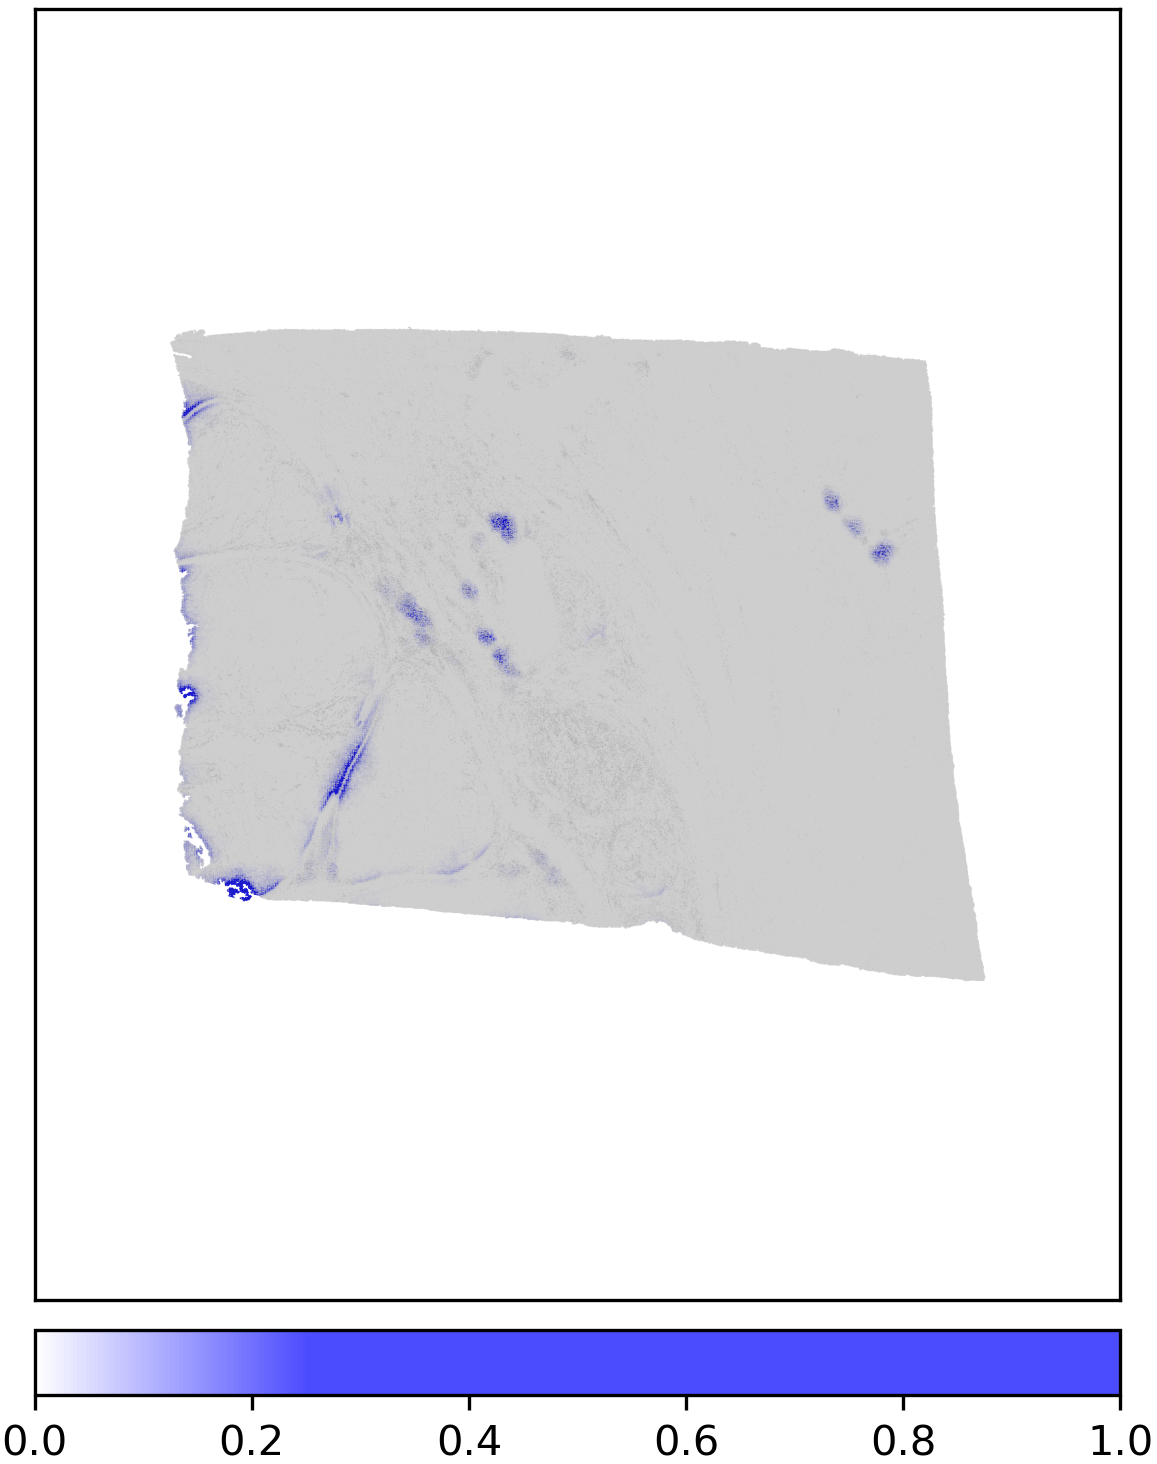
\includegraphics[width=\textwidth]{latex/captum/case13/integrated_gradients_abs_case13-stain41-dead_2415days.png}
         \caption{Integrated Gradients, abs. attributions}
     \end{subfigure}
\vskip\baselineskip
     \begin{subfigure}[b]{0.49\textwidth}
         \centering
         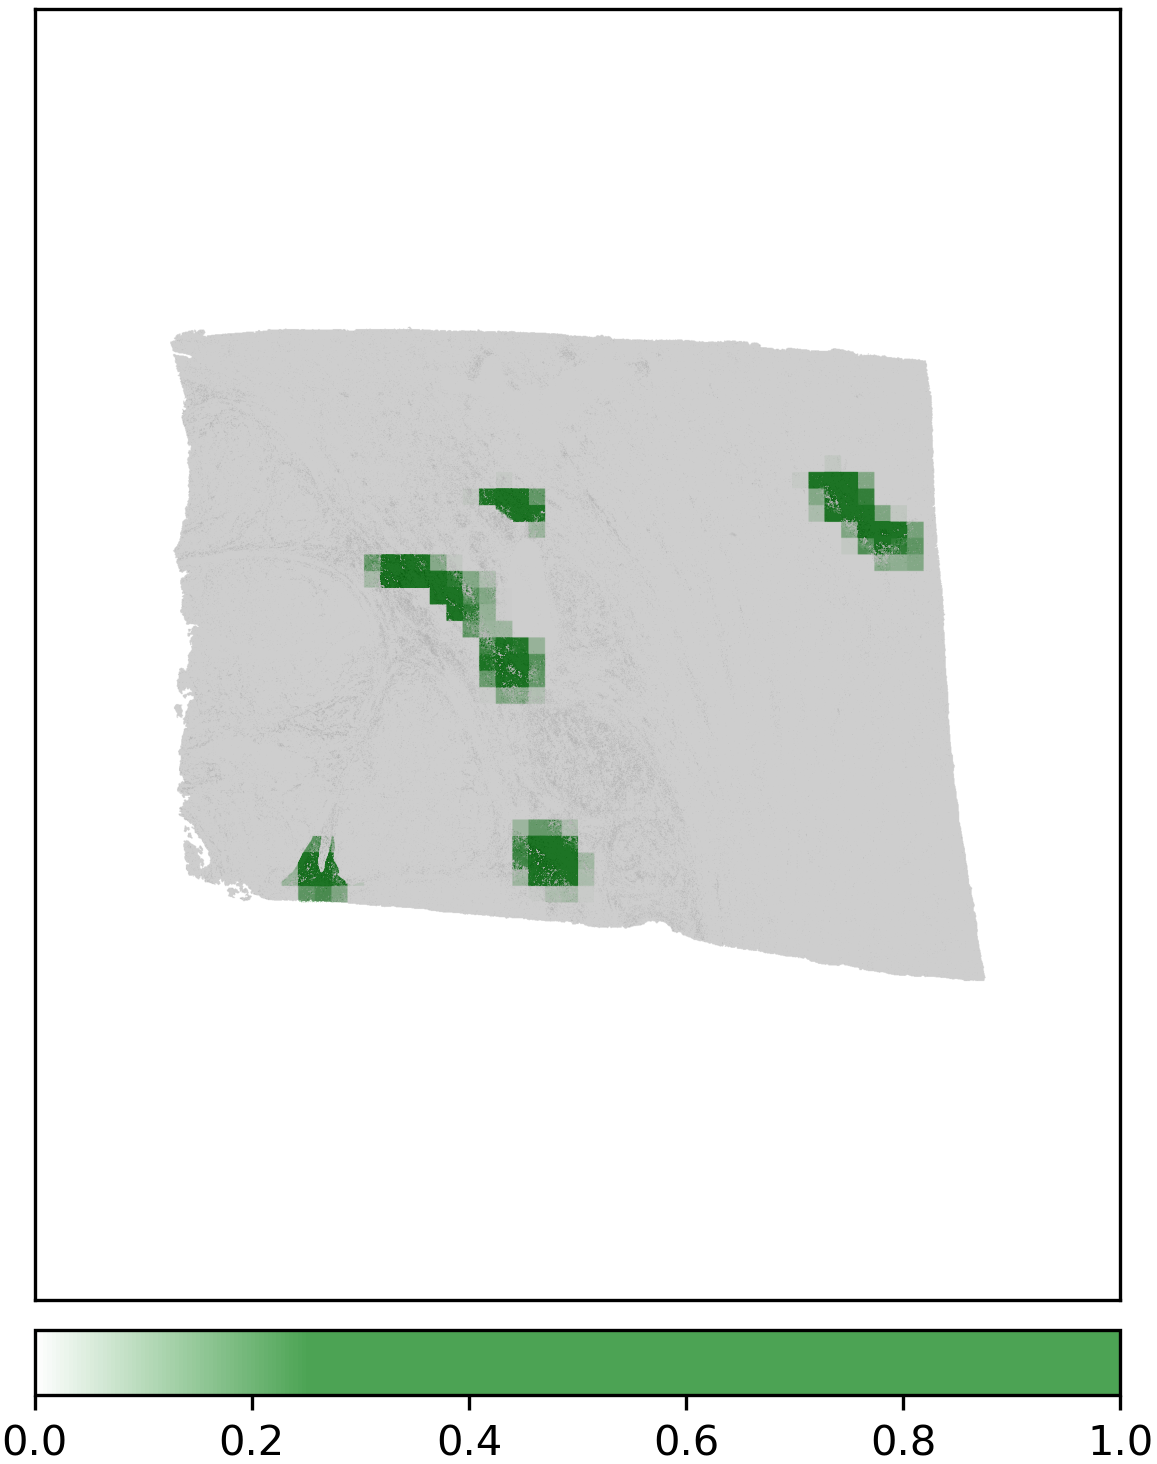
\includegraphics[width=\textwidth]{latex/captum/case13/guided_gradcam_pos_case13-stain41-dead_2415days.png}
         \caption{Guided GradCAM, positive attributions}
     \end{subfigure}
    \hfill
     \begin{subfigure}[b]{0.49\textwidth}
         \centering
         \includegraphics[width=\textwidth]{latex/captum/case13/guided_gradcam_neg_case13-stain41-dead_2415days.png}
         \caption{Guided GradCAM, negative attributions}
     \end{subfigure}
    \hfill
    \caption[Integrated gradients and Guided GradCAM for case 13  stain 41]{Results of Integrated Gradients and Guided GradCAM for case 13  stained for CD8 and CD20. The figure of the tumour masks is included for comparison. Integrated Gradients attributions are converted to absolute values.}
    \label{fig:case13a}
\end{figure}


\begin{figure}[h!t]
    \centering
     \begin{subfigure}[b]{0.475\textwidth}
         \centering
         \includegraphics[width=\textwidth]{latex/captum/case13/masks_case13-stain41-dead_2415days.png}
         \caption{Tumour annotations of WSI}
     \end{subfigure}
    \hfill
     \begin{subfigure}[b]{0.49\textwidth}
         \centering
         \includegraphics[width=\textwidth]{latex/captum/case13/Occlusion_abs_case13-stain41-dead_2415days.png}
         \caption{Occlusion map; kernel and stride of 50}
     \end{subfigure}
\vskip\baselineskip
     \begin{subfigure}[b]{0.49\textwidth}
         \centering
         \includegraphics[width=\textwidth]{latex/captum/case13/saliency_case13-stain41-dead_2415days.png}
         \caption{Saliency Maps}
     \end{subfigure}
    \hfill
     \begin{subfigure}[b]{0.49\textwidth}
         \centering
         \includegraphics[width=\textwidth]{latex/captum/case13/inputXgradient_pos_case13-stain41-dead_2415days.png}
         \caption{Input*Gradient}
     \end{subfigure}
  
    \hfill
    \caption[Occlusion and Saliency for case 13  stain 41]{Results of Saliency, Input*Gradients and occlusion mapping for case 13. The figure of the tumour masks is included for comparison. All attributions were converted to absolute values.}
    \label{fig:case13b}
\end{figure}

\begin{figure}[h!t]
    \centering
     \begin{subfigure}[b]{0.475\textwidth}
         \centering
         \includegraphics[width=\textwidth]{latex/captum/case13b/masks_case13-stain42-dead_2415days.png}
         \caption{Tumour annotations of WSI}
     \end{subfigure}
    \hfill
     \begin{subfigure}[b]{0.49\textwidth}
         \centering
         \includegraphics[width=\textwidth]{latex/captum/case13b/integrated_gradients_abs_case13-stain42-dead_2415days.png}
         \caption{Integrated Gradients, abs. attributions}
     \end{subfigure}
\vskip\baselineskip
     \begin{subfigure}[b]{0.49\textwidth}
         \centering
         \includegraphics[width=\textwidth]{latex/captum/case13b/guided_gradcam_pos_case13-stain42-dead_2415days.png}
         \caption{Guided GradCAM, positive attributions}
     \end{subfigure}
    \hfill
     \begin{subfigure}[b]{0.49\textwidth}
         \centering
         \includegraphics[width=\textwidth]{latex/captum/case13b/saliency_case13-stain42-dead_2415days.png}
         \caption{Saliency Map, abs. attributions}
     \end{subfigure}
    \hfill
    \caption[Integrated gradients, Guided GradCAM and saliency for case 13 stain 42]{Results of Integrated Gradients and Guided GradCAM for case 13 stained for CD4 and FoxP3. The figure of the tumour masks is included for comparison. Integrated Gradients attributions are converted to absolute values.}
    \label{fig:case13c}
\end{figure}


\begin{figure}[h!t]
    \centering
     \begin{subfigure}[b]{0.475\textwidth}
         \centering
         \includegraphics[width=\textwidth]{latex/captum/case129/masks_case129-stain19-dead_414days.png}
         \caption{Tumour annotations of WSI}
     \end{subfigure}
    \hfill
     \begin{subfigure}[b]{0.49\textwidth}
         \centering
         \includegraphics[width=\textwidth]{latex/captum/case129/integrated_gradients_abs_case129-stain19-dead_414days.png}
         \caption{Integrated Gradients, abs. attributions}
     \end{subfigure}
\vskip\baselineskip
     \begin{subfigure}[b]{0.49\textwidth}
         \centering
         \includegraphics[width=\textwidth]{latex/captum/case129/guided_gradcam_pos_case129-stain19-dead_414days.png}
         \caption{Guided GradCAM, positive attributions}
     \end{subfigure}
    \hfill
     \begin{subfigure}[b]{0.49\textwidth}
         \centering
         \includegraphics[width=\textwidth]{latex/captum/case129/saliency_case129-stain19-dead_414days.png}
         \caption{Saliency Map, abs. attributions}
     \end{subfigure}
    \hfill
    \caption[Integrated gradients, Guided GradCAM and saliency for case 129 stain 19]{Results of Integrated Gradients and Guided GradCAM for case 129 stained for CD204. The figure of the tumour masks is included for comparison. Integrated Gradients and saliency attributions are converted to absolute values.}
    \label{fig:case129}
\end{figure}

% 001 = HE-Elastika
% 016 = CD68 (Makrophagen)
% 019 = CD204 (TAM)
% 041 = CD8_CD20
% 042 = CD4_FoxP3
